\chapter{$\Dsplus$ production in Pb-Pb collisions at $\s$ = 5.02 TeV}
In 2011 ALICE $\PbPb$ events were collected using different trigger configurations: $central$, $semi-central$ and $minimum-bias$.  The $central$ trigger is based on the information of the Silicon Pixel Detector and the VZERO detector. Its efficiency for hadronic interactions was 100$\%$ for the 7.5$\%$ most central events.  About 30$\times 10^6$ events passed the central trigger criteria. The analyzed data sample, for the $\pt$ dependent analysis in the semicentral  class, consists of a logical OR between the semi central and minimum bias trigger.

\section{v2 requests}
{\bf Event selection}: AOD events were selected using the physics selection and requiring the primary vertex to be reconstructed from tracks with a z coordinate in the range $|z|<10$~cm.

{\bf Triggers}: In 2015 ALICE $\PbPb$ events were collected using the $minimum-bias$ trigger configuration, based on the information of the Silicon Pixel Detector and the VZERO detector. 

{\bf Centrality estimator:} Multiplicity in the VZERO detector. Track 
multiplicity used to cross-check. The analysis is performed in the
centrality class 30--50\%. The number of analyzed events was $20.65$
millions for the centrality class 30--50\%, corresponding to an
integrated luminosity of 13.4 $\mu$b$^{-1}$.


\section{Single track selection}

Secondary vertices of $\Dzero$ and $\Dplus$ meson candidates were constructed using tracks
having $|\eta| < 0.8$, $\pt > 0.5$ GeV/c and passing the kITSrefit and kTPCrefit conditions. 
Moreover, for all the tracks,  a minimum number of 70 crossed rows in the TPC together with a crossed rows over findable clusters ratio of 0.8 was required.
A cut on the transverse impact parameter $d_0$ was applied for tracks with $\pt < 2$ GeV/c, requiring $d_0 >50 \mu m$. These selections
were meant to limit the CPU time needed to perform the track combinatorics when creating the
AODs with the D meson candidates. Furthermore, all tracks, including the $\Dstar$ soft pion, were 
selected requiring at least
70 (out of a maximum of 159) associated space points and $\chi^2/ndf < 2$ in the TPC, and
at least one associated hit in either of the two pixel layers. 
\section{D mesons selection strategy}

%Ds
\begin{table}[!h]
 \caption{List of the main topological selections applied for the
   $\Ds$ analysis in 30-50\% centrality class FOR v2 ANALYSIS.}
 \label{Ds_cuts}
 \begin{center}
  \begin{tabular}{|c|c|c|c|c|c|}
\hline
$\pt$ (GeV/c)/variable & [2,4] & [4,6] & [6,8] & [8,12] & [12,16] \\
\hline
\hline
Decay length ($\mum$)        & $>$400 & $>$500 & $>$500 & $>$500 & $>$400\\
\hline
Decay length XY ($\mum$)     & $>$300 & $>$500 & $>$500 & $>$500 & $>$300\\
\hline
Norm Decay length XY          & $>$9.0& $>$7.0 & $>$7.0 & $>$6.0 & $>$6.0\\
\hline
Cosine pointing              & $>$0.997 & $>$0.99 & $>$0.98 & $>$0.98 & $>$0.99\\
\hline
Cosine pointing XY        & $>$0.997 & $>$0.99 & $>$0.98 & $>$0.98 & $>$0.99\\
\hline
$\sigma_{vertex}$  (cm)          & $<$0.020 & $<$0.020 & $<$0.025 & $<$0.030 & $<$0.025\\
\hline
M$^{\phi}_{inv}$ - M$^{\phi PDG}_{inv}$ (MeV/$c^{2}$) & $<$4.0 & $<$6.0 & $<$6.0 & $<$4.0 & $<$6.0\\
\hline
$\cos \theta^*(\pi)$    & $<$0.80 & $<$0.70 & $<$0.85 & $<$0.85 & $<$0.75\\
\hline
$|\cos^3 \theta^\prime({\rm K})|$        & $>$0.20 & $>$0.15 & $>$0.05 & $>$0.10 & $>$0.00\\
\hline
Norm. IP residual   & $<$1.5 & $<$1.5 & $<$2.5 & $<$2.5 & $<$2.5 \\
\hline
  \end{tabular}
 \end{center}
\end{table} 

From Table t we report the topological selections applied for each meson in the 0-10$\%$ and 60-80$\%$ centrality classes.
\begin{table}[!h]
 \caption{List of the main topological selections applied for the
   $\Ds$ analysis in 0-10\% centrality class.}
 \label{topologicalselections_ds_010}
 \begin{center}
  \begin{tabular}{|c|c|c|c|c|}
\hline
$\pt$ (GeV/c)/variable &  [4,6] & [6,8] & [8,12] & [12,16] \\
\hline
\hline
Decay length ($\mum$)        & $>$500 & $>$500 & $>$400 & $>$400\\
\hline
Decay length XY ($\mum$)     & $>$500 & $>$500 & $>$400 & $>$400\\
\hline
Norm Decay length XY          & $>$9.0 & $>$9.0 & $>$6.0 & $>$8.0\\
\hline
Cosine pointing              & $>$0.995 & $>$0.99 & $>$0.98 & $>$0.99\\
\hline
Cosine pointing XY        & $>$0.995 & $>$0.99 & $>$0.98 & $>$0.99\\
\hline
$\sigma_{vertex}$  (cm)          &  $<$0.025 & $<$0.030 & $<$0.025 & $<$0.025\\
\hline
M$^{\phi}_{inv}$ - M$^{\phi PDG}_{inv}$ (MeV/$c^{2}$) & $<$6.0 & $<$5.0 & $<$4.0 & $<$4.0\\
\hline
$\cos \theta^*(\pi)$    &$<$0.80 & $<$1.00 & $<$0.80 & $<$0.90\\
\hline
$|\cos^3 \theta^\prime({\rm K})|$        & $>$0.20 & $>$0.10 & $>$0.20 & $>$0.10\\
\hline
Norm. IP residual   & $<$1.0 & $<$2.0 & $<$2.0 & $<$2.5 \\[1ex]
\hline
  \end{tabular}
 \end{center}
\end{table} 
\begin{table}[!h]
 \caption{List of the main topological selections applied for the
   $\Ds$ analysis in 60-80\% centrality class.}
 \label{topologicalselections_ds_6080}
 \begin{center}
  \begin{tabular}{|c|c|c|c|c|c|}
\hline
$\pt$ (GeV/c)/variable & [2,4] & [4,6] & [6,8] & [8,12] & [12,16] \\
\hline
\hline
Decay length ($\mum$)                 & $>$300 & $>$400 & $>$400 & $>$500 & $>$400\\
\hline
Decay length XY ($\mum$)            & $>$300 & $>$400 & $>$400 & $>$500 & $>$400\\
\hline
Norm Decay length XY                   & $>$7.0& $>$6.0 & $>$8.0 & $>$4.0 & $>$1.0\\
\hline
Cosine pointing                               & $>$0.99 & $>$0.98 & $>$0.98 & $>$0.97 & $>$0.995\\
\hline
Cosine pointing XY                          & $>$0.99 & $>$0.98 & $>$0.98 & $>$0.97 & $>$0.995\\
\hline
$\sigma_{vertex}$  (cm)                   & $<$0.030 & $<$0.030 & $<$0.025 & $<$0.015 & $<$0.030\\
\hline
M$^{\phi}_{inv}$ - M$^{\phi PDG}_{inv}$ (MeV/$c^{2}$) & $<$5.0 & $<$10.0 & $<$7.0 & $<$10.0 & $<$5.0\\
\hline
$\cos \theta^*(\pi)$                             & $<$0.70 & $<$0.80 & $<$1.00 & $<$1.00 & $<$1.00\\
\hline
$|\cos^3 \theta^\prime({\rm K})|$        & $>$0.05 & $>$0.1 & $>$0.00 & $>$0.00 & $>$0.00\\
\hline
Norm. IP residual                               & $<$3.0 & $<$3.0 & $<$3.0 & $<$5.0 & $<$2.5 \\[1ex]
\hline
  \end{tabular}
 \end{center}
\end{table}
\subsubsection{Particle identification}

 The selection is that usually preferred for the $\Ds$ meson, used here for $\pt$ between 4 and 12 $\GeV/c$ for the 0--10\% centrality and in the
full $\pt$ interval for the 60--80\% interval. In particular, a track was considered compatible with the kaon or pion hypothesis if both its dE/dx and time-of-flight were within 3$\sigma$ from the expected values. 
Tracks without a TOF signal (mostly at low momentum) were identified using only the TPC information and requiring a 2$\sigma$ compatibility with the expected dE/dx. Triplets of selected tracks were required to have two tracks compatible with the pion hypothesis and one with the kaon hypothesis. In addition, since the decay particle with opposite charge sign has to be a kaon, a triplet was rejected if the opposite-sign track was not compatible with the kaon hypothesis. This strategy still preserves about 85$\%$ of the $\Ds$ and of the $\Dplus$ signal in the $\pt$ interval where it is used.
\subsection{Signal extraction}
 The signal in the 0-10$\%$centrality class was extracted in the transverse
momentum region 4-16 GeV$/c$ for the $\Ds$ meson; in the 60-80$\%$centrality class the $\pt$ region is 2-16 GeV$/c$ for the $\Ds$ meson.\\
Fig. for the 60-80$\%$ centrality class.

\begin{figure}[!htbp]
 \begin{center}
  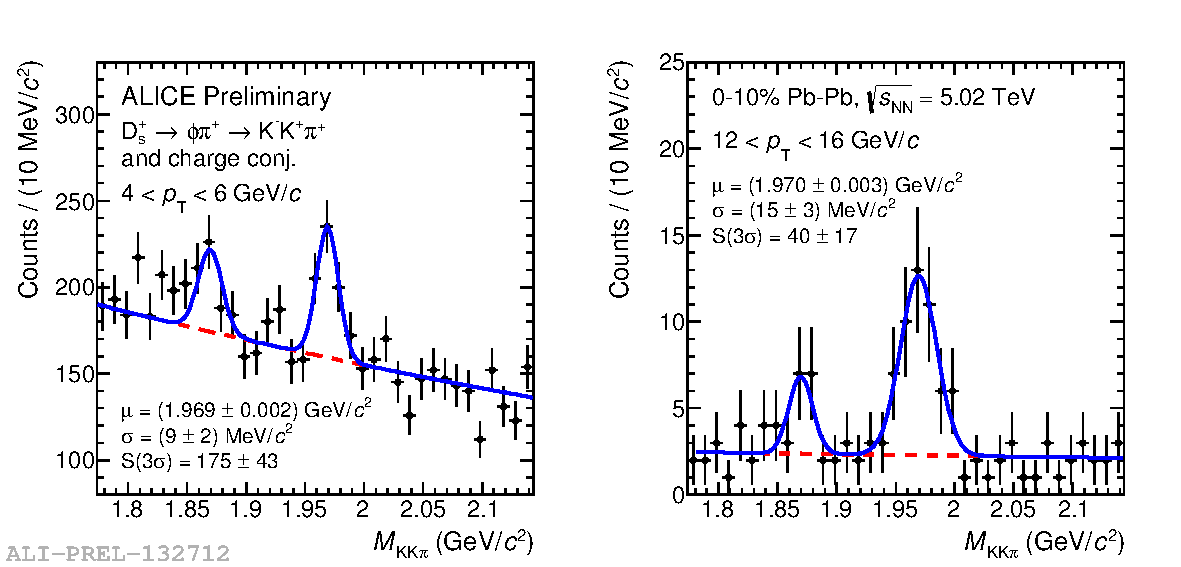
\includegraphics[width=.9\textwidth]{FigCap5/MassDs_PbPb010_5TeV_pt_4-6_12-16.pdf}
\end{center}
 \caption{$\Ds$ signal in 4 $\pt$ bins in the range, $4<\pt<16$ GeV$/c$ for the 0-10$\%$ centrality class. }
 \label{FigInvMassDs_010} 
\end{figure} 
 
\begin{figure}[!htbp]
 \begin{center}
  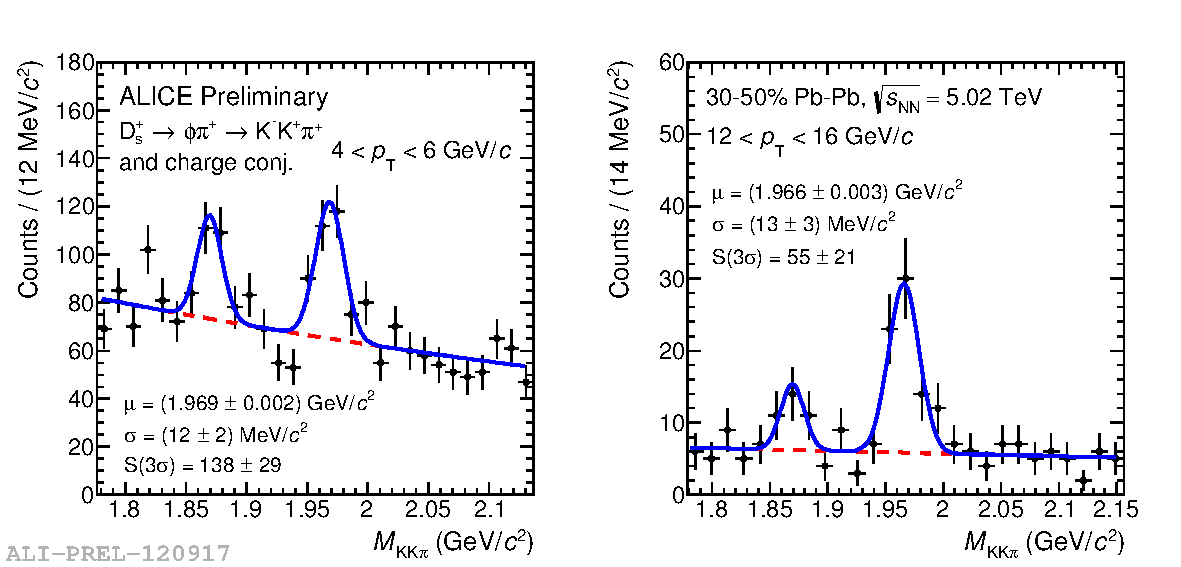
\includegraphics[width=.9\textwidth]{FigCap5/MassDs_PbPb3050_5TeV_pt_4-6_12-16.pdf}
\end{center}
 \caption{$\Ds$ signal in 4 $\pt$ bins in the range, $4<\pt<16$ GeV$/c$ for the 30-50$\%$ centrality class. }
 \label{FigInvMassDs_3050} 
\end{figure} 
 
\begin{figure}[!h]
 \begin{center}
  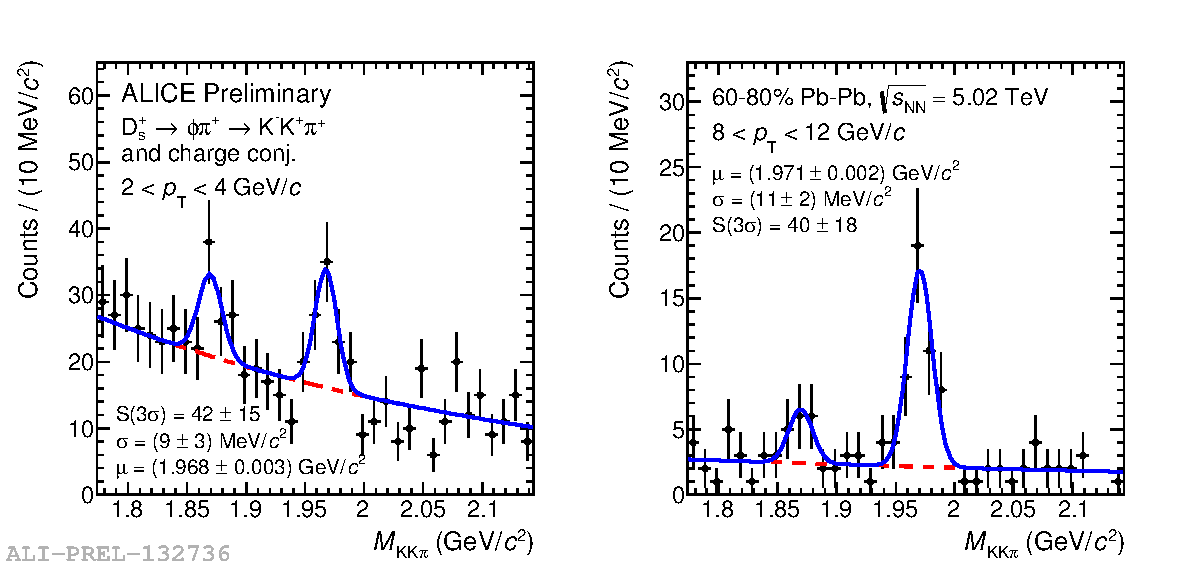
\includegraphics[width=.9\textwidth]{FigCap5/MassDs_PbPb6080_5TeV_pt_2-4_8-12.pdf}
\end{center}
 \caption{$\Ds$ signal in 4 $\pt$ bins in the range, $4<\pt<16$ GeV$/c$ for the 60-80$\%$ centrality class. }
 \label{FigInvMassDs_6080} 
\end{figure} 
 

\begin{figure}[!ht]
 \begin{center}
  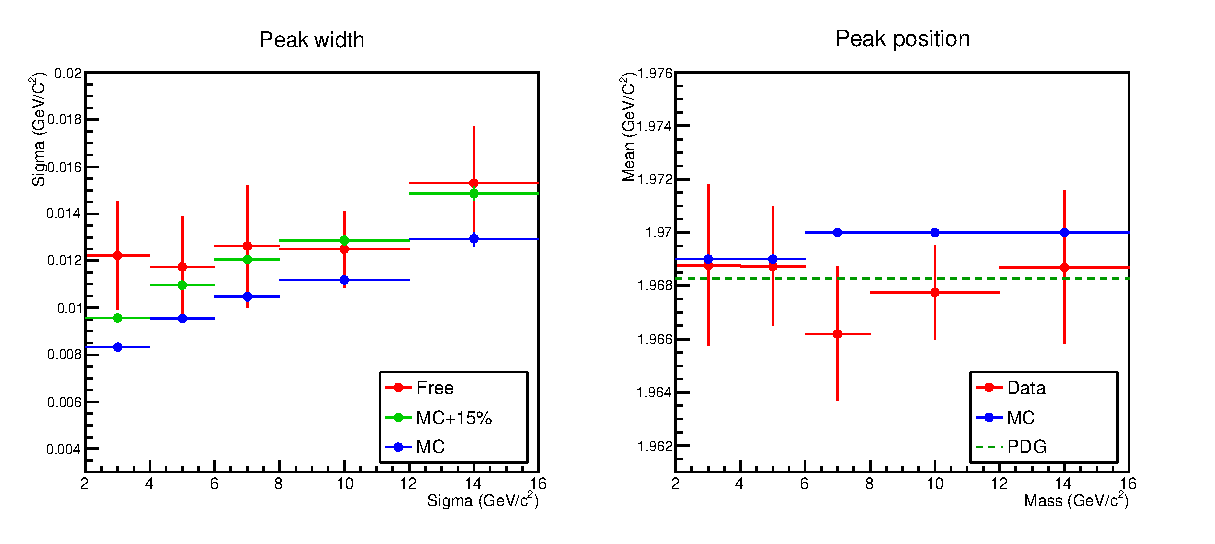
\includegraphics[angle=0, width=15cm]{./FigCap5/MeanSigma_DataMC.eps}
 \end{center}
 \caption{Width (left) and mean (right) of the $\Ds$ signal peak and as a function of $\pt$: comparison data (red), Monte Carlo (blue) and Monte Carlo + 15\% (green). }
 \label{MCsigmacheckDs} 
\end{figure} 


\iffalse
 \begin{table}[!htbp]
 \caption{$\Ds$ raw yields and signal over background per $\pt$ bin for the 0-10$\%$ and 60-80$\%$ centrality classes.}
 \label{signalDs_010_6080}
 \begin{center}
  \begin{tabular}{|c|c|c|c|c|}
\hline
\multirow{2}{*}{$\pt$ bin (GeV$/c$)} & \multicolumn{2}{c|}{0-10$\%$} & \multicolumn{2}{c|}{60-80$\%$} \\
\cline{2-5}
& raw yield & S/B & raw yield & S/B \\
\hline
\hline
[2,4] & -  & - & 42 $\pm$ 12 & 0.47 \\
\hline
[4,6] &  176 $\pm$ 32  & 0.20 & 113 $\pm$ 17 & 0.63\\
\hline
[6,8] &  195 $\pm$ 36  & 0.16 & 33 $\pm$ 7 & 3.08 \\
\hline
[8,12] & 137 $\pm$ 28 & 0.23 & 40 $\pm$ 7 & 2.95 \\
\hline
[12,16] & 40 $\pm$ 8  & 1.90 & 16 $\pm$ 5 & 2.10 \\
\hline
  \end{tabular}
 \end{center}
\end{table} 
\fi
\section{D mesons efficiencies}

The prompt D meson production yields were calculated by correcting the measured inclusive raw yields, 
$N^{\rm raw}$, for 
the B meson decay feed-down contribution and dividing by the acceptance times 
efficiency for prompt D mesons, $({\rm Acc}\times\epsilon)_{\rm prompt}$. 
They were normalized according to the decay channel  branching ratio ({\rm BR}), $\pt$ interval width ($\Delta \pt$), rapidity coverage 
($\Delta y$), and the number of events analyzed ($N_{\rm evt}$). They were then divided by a factor of two to evaluate the charge (particle and anti-particle) averaged yields. As an illustration, the ${\rm D^+}$  yields were computed as:
\begin{equation}
  \label{eq:dNdpt}
  \left.\frac{{\rm d} N^{\rm D^+}}{{\rm d}\pt}\right|_{|y|<0.5}=
  \frac{1}{2}\frac{1}{ \Delta y \,\Delta \pt}\frac{\left.f_{\rm prompt}(\pt)\cdot N^{\rm D^\pm~raw}(\pt)\right|_{|y|<y_{\rm fid}}}{({\rm Acc}\times\epsilon)_{\rm prompt}(\pt) \cdot{\rm BR} \cdot N_{\rm evt}}\,.
\end{equation}
Where $f_{prompt}$ is the prompt D meson fraction in a given $\pt$ bin. The D meson yields were measured in a rapidity range varying 
from $|y|<0.5$ at low $\pt$ to $|y|<0.8$ at high $\pt$.
The rapidity acceptance correction factor $\Delta y=2\,y_{\rm fid}$ assumes
a uniform rapidity  distribution for D mesons in the measured $y$ range.
This assumption was verified to the $1\%$ level with PYTHIA proton--proton simulations 
with the Perugia-0 tuning. The acceptance times efficiency corrections ${\rm Acc}\times\epsilon$ 
were obtained using Monte Carlo simulations. 
Minimum-bias Pb--Pb collisions at $\sqrtsNN=5.02~\tev$
were produced with the HIJING~v1.36 event generator.
Prompt and feed-down (B decays) D meson signals were added using pp events from the PYTHIA~v6.4.21 
event generator with the Perugia-0 tuning. 
Each injected pp event was required to contain a $\rm c\overline c$ or $\rm b\overline b$ pair and D mesons
were forced to decay in the hadronic channels of interest for the analysis. Only particle coming from the heavy quark hadronization and decays were injected in the HIJING event. The number of pp events added to each Pb--Pb event was adjusted according to the Pb--Pb collision centrality. The simulations used the GEANT3 particle transport package together with a detailed description of the geometry of the apparatus and of the detector response.
The simulation was configured to reproduce the conditions of the luminous region and of all the ALICE subsystems, 
in terms of active electronic channels, calibration level, and their time evolution within the Pb--Pb data taking period. 

Studies on the impact parameter resolution on the 2015 data sample, revealed that this resolution is slightly worse (by about 5-10 micron at all $\pt$s) than in Run-1 (e.g. 2011 Pb-Pb data).
The impact parameter distribution is shifted to negative values by up to 20-30 micron at low $\pt$ and decreasing to 5-10 micron at high $\pt$. The shift depends on the azimuthal angle and is not described in the MC. Current hypothesis is that part of the shift is due to the presence of SPD modules that were not included in the latest realignment (because they were included only recently in the data taking). The task scales in the MC the residuals d0(true)-d0(reco) according to the ratio data/MC of the impact parameter resolutions .


The efficiencies were evaluated in a centrality class corresponding to the one used in the analysis of the data in terms of charged particle 
multiplicity, hence of the detector occupancy.
Some of the topological selections tend to reject less feed-down due to the larger 
decay length with respect to the prompt D mesons. This is the reason why the feed-down 
efficiency is overall a bit higher than the prompt at low $\pt$ for $\Dzero$, $\Dstar$ and $\Ds$ mesons.
Other topological cuts, like the one on the normalised track-impact parameter, are more effective
in rejecting the feed-down component, allowing higher prompt efficiencies at high $\pt$ or in the $\Dplus$ meson case.

\begin{figure}[!t]
%\begin{center}
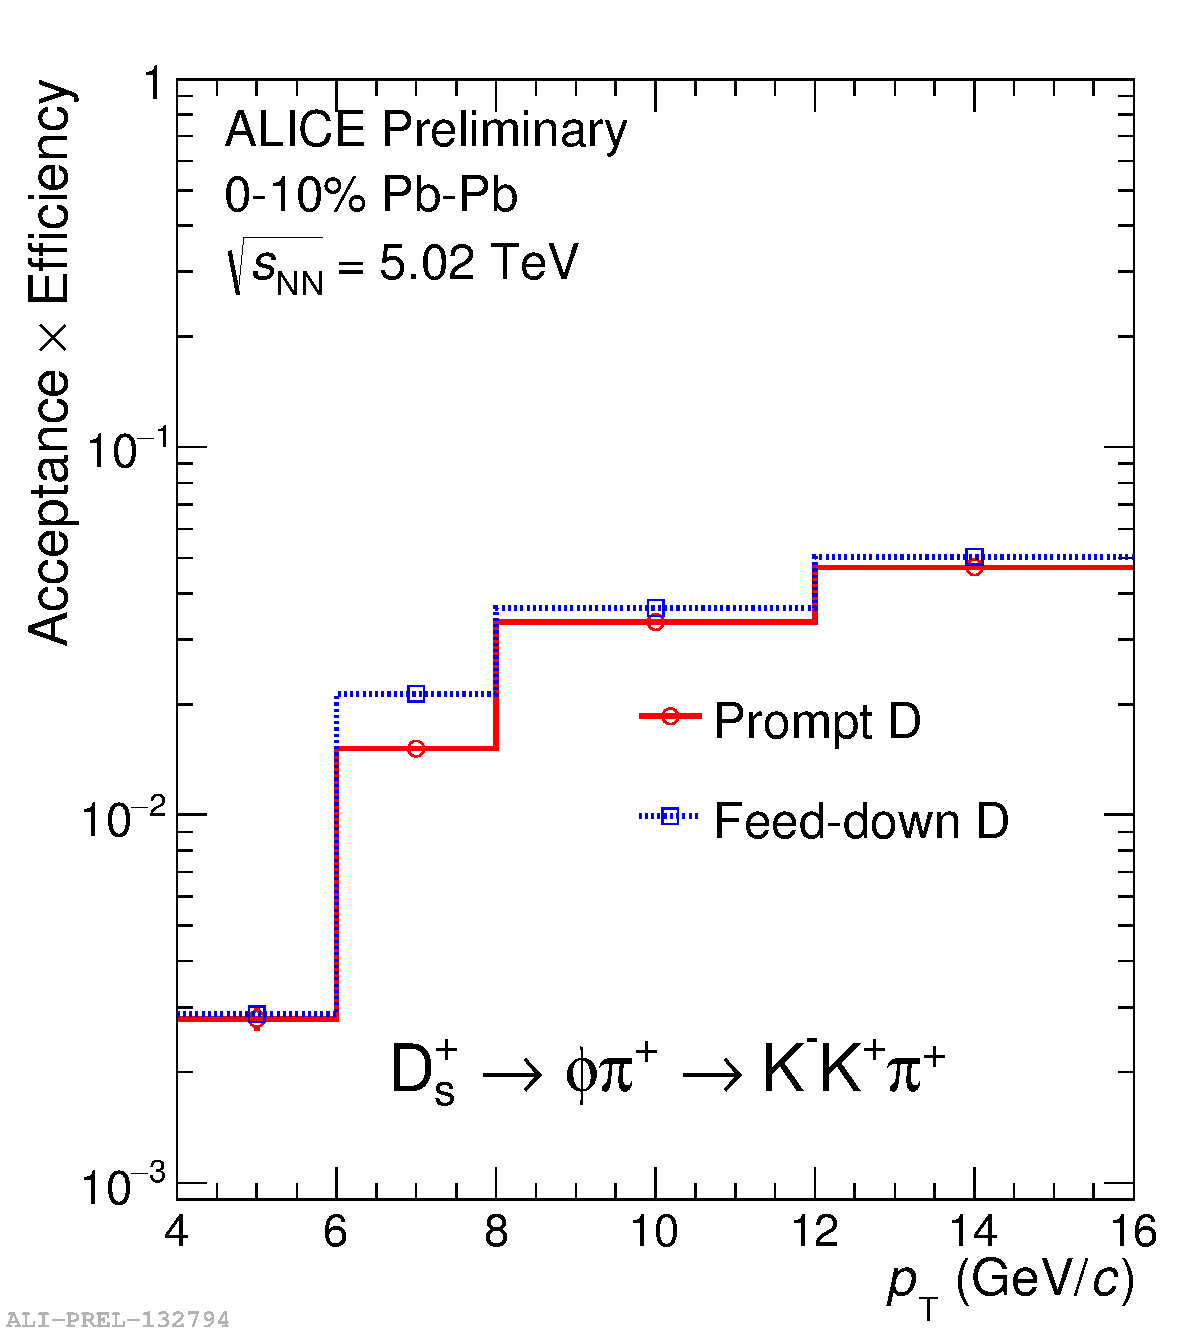
\includegraphics[width=.49\textwidth]{FigCap5/AccEff_Ds_010.pdf}
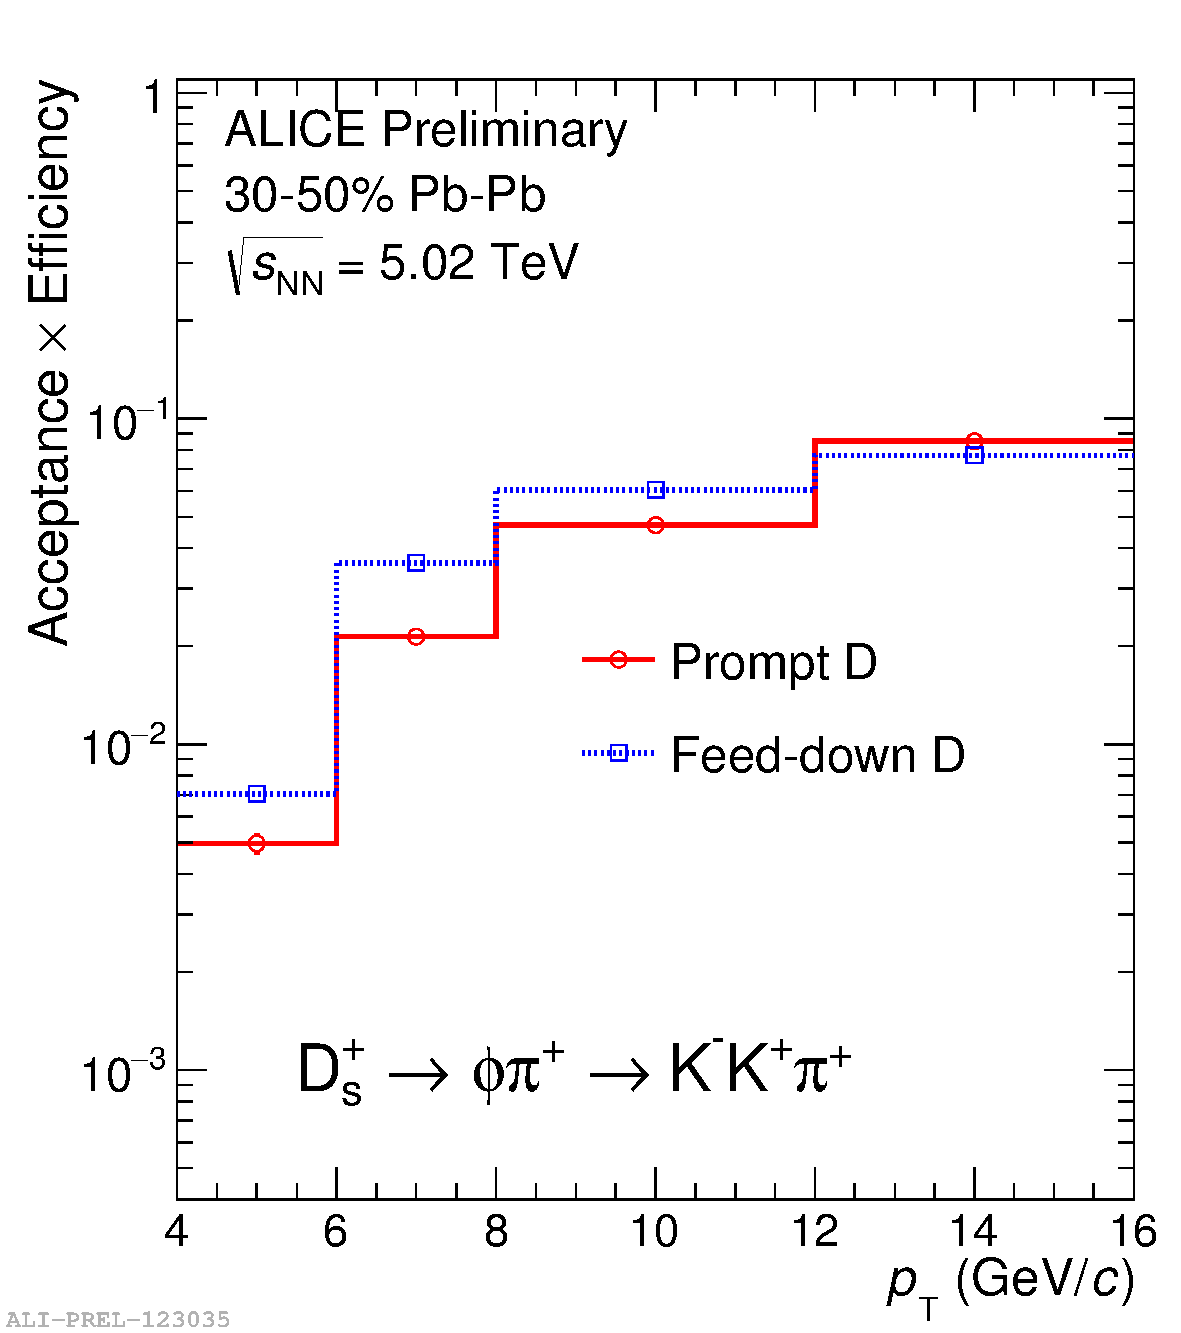
\includegraphics[width=.49\textwidth]{FigCap5/AccEff_Ds_3050.pdf}
%\end{center}
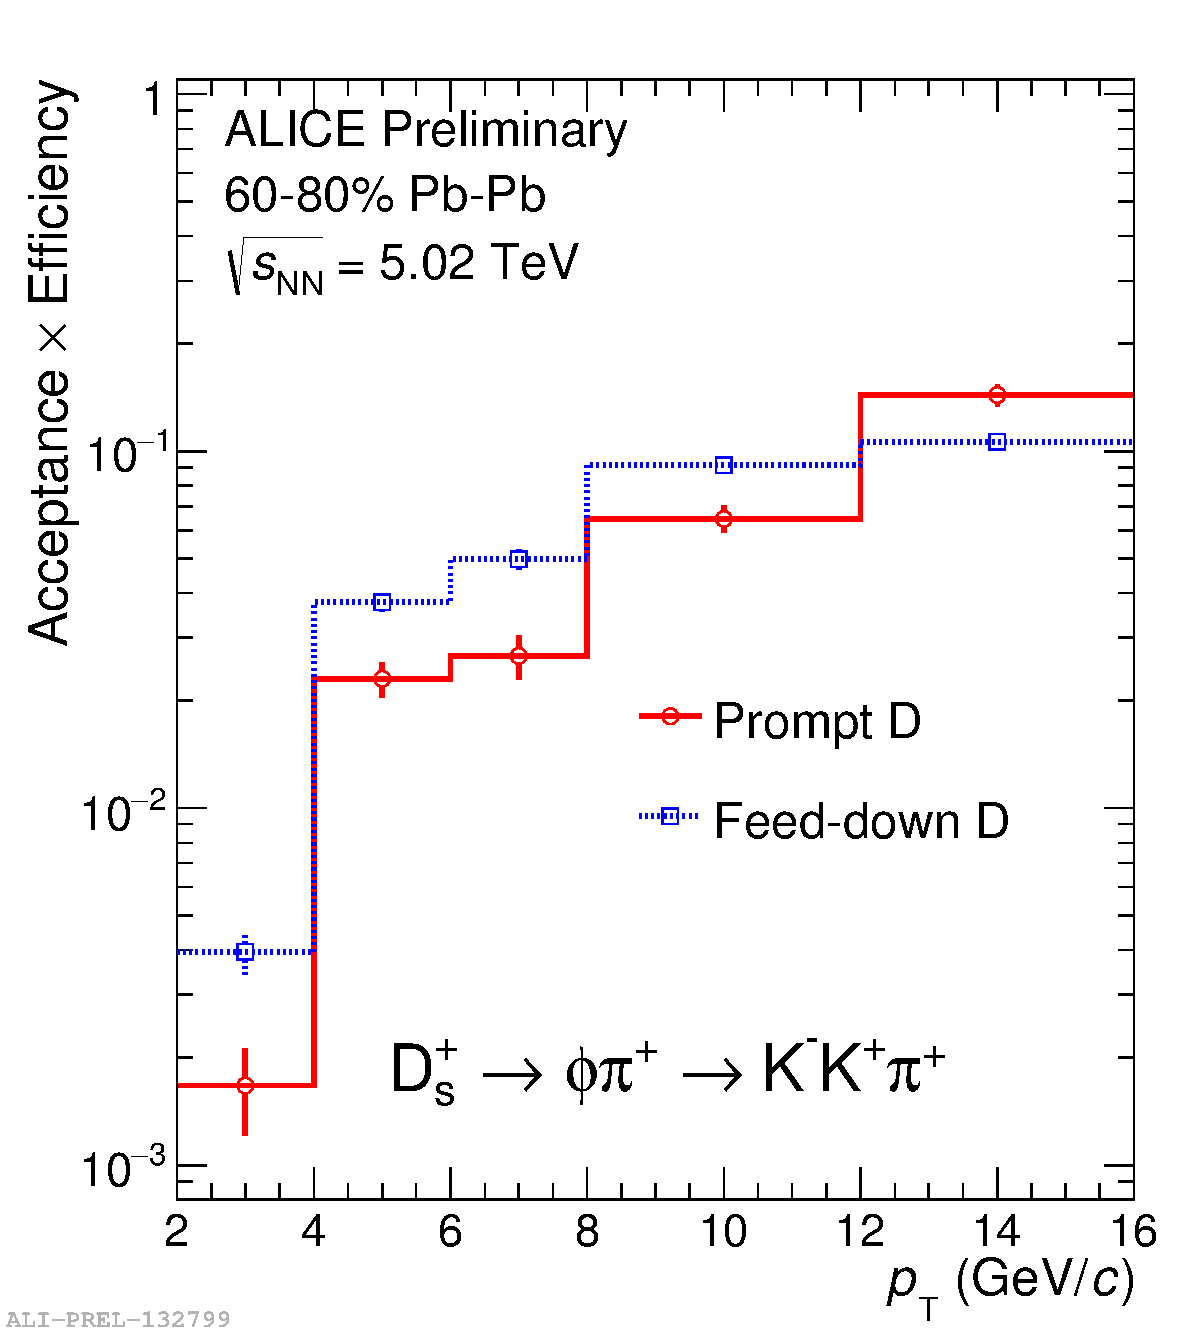
\includegraphics[width=.49\textwidth]{FigCap5/AccEff_Ds_6080.pdf}
\caption{Efficiency times acceptance for $\Ds$ mesons in the 30-50\% centrality range, as a function of $\pt$, for prompt (red) and feed-down (blue) $\Ds$.}
\label{fig:DsAccEff}
\end{figure}

\section{Event plane based methods}
The determination of the event plane in ALICE can be performed using
either the tracks reconstructed in the TPC, which has an uniform
azimuthal coverage in the central rapidity region, or the V0
detectors, located at forward ($2.8<\eta<5.1$) and backward
($-3.7<\eta<-1.7$) pseudorapidity.

The event plane angle $\psi_n$ is an estimator of the reaction
plane angle ($\Psi_{\rm RP}$), i.e. the true reaction plane formed by
the impact parameter of the two colliding nuclei and the beam
direction. Due to the finite number of detected particles, the
resolution in angle is limited and can be estimated for each harmonic
considered. The measured $v_n^{\rm obs}$ must be divided by the
resolution term to obtain the real $v_n$.

\subsection{Event plane determination}\label{TPCEP}
The basic quantity that is needed to study azimuthal anisotropy is the estimate of the reaction-plane angle, which is defined by the vector of the impact parameter and the beam direction. The reaction-plane angle can not be directly measured, but can be estimated from the particle azimuthal distribution event-by-event. 

The orientation of the reaction plane or, in case of flow fluctuations, the $n^{\rm th}$-harmonic collision symmetry plane is estimated with the $n^{\rm th}$-harmonic event-plane angle, $\psi_n$. For a given harmonic $n$, one constructs the two-dimensional event-plane vector $Q_n$ from the measured azimuthal distribution of particles produced in the event as follows:

\begin{equation}\label{f:qvector}
 Q_n={\sum_{i=0}^{N} w_i \cos n\phi_i \choose \sum_{i=0}^{N} w_i \sin n\phi_i} \qquad \psi_n = \dfrac{1}{n} \tan^{-1} \left(\dfrac{Q_{n,y}}{Q_{n,x}}\right).
\end{equation}

The sums run over all reconstructed tracks in the case of the TPC, or segments of detectors with azimuthal segmentation like VZERO, FMD, ZDC, or PMD. The angle $\varphi_i$ is the azimuthal emission angle of the particle $i$ or the azimuthal coordinate of the detector element $i$, respectively. For TPC tracks the weight $w_i$ can be unity or a specific function of $\pt$. For segmented detectors, $w_i$ is the signal observed in the detector element $i$. Using the components of the $Q$-vector one can calculate the $\psi_n$.

In order to get  the real $v_n$, the  $v_n^{\rm obs}$ must be divided by the resolution ($R_n$) which can be expressed as \cite{Poskanzer:1998yz}:
\begin{equation}
\label{f:epreso}
\left\langle \cos km\left( \psi_m-\Psi_{\rm RP}\right)\right\rangle = \sqrt{\dfrac{\pi }{8}} \chi_m \cdot {\rm e}^{-\chi_m^2/4} \cdot I_{(k-1)/2}(\chi_m^2/4)+I_{(k+1)/2}(\chi_m^2/4),
\end{equation}
where $\chi_m=v_n\sqrt{2N}$ ($N$ is the multiplicity) and $I_\nu$ the Bessel function of order $\nu$, as drawn in Fig.~\ref{fig:resoBessel}.
$k$ is an integer number that accounts for the fact that the event plane of $m$-th order can be used to compute all Fourier harmonics that are multiples
of $m$ (i.e. $km$).
The mean cosine values are less than one, thus the correction always increases the Fourier coefficients.

\begin{figure}
\centering
 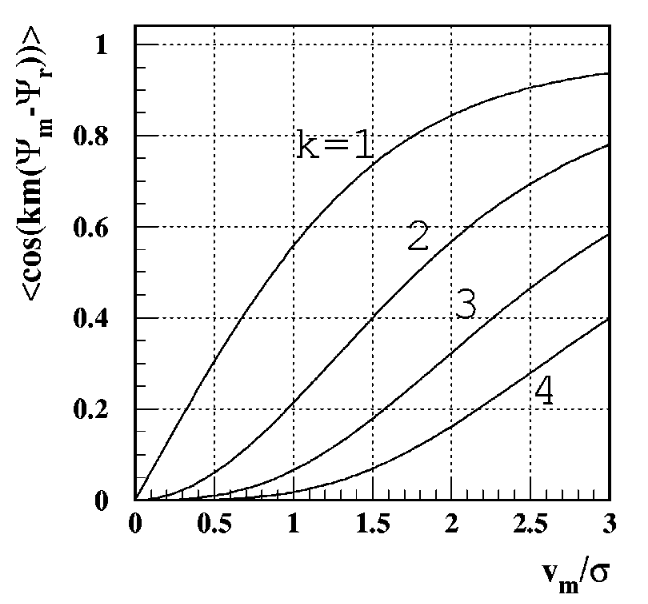
\includegraphics[width=0.5\textwidth]{FigCap5/resolBessel.png}
 \caption[Event plane resolution vs $\chi_m$]{The event plane resolution for the $n$-th ($n=km$, according the conventions of eq.~(\ref{f:epreso})) harmonic of the particle distribution with respect to the $m$-th harmonic plane, as a function of $\chi_m$ (figure taken from).}
 \label{fig:resoBessel}
\end{figure}

The resolution can be measured from data using two sub-events, i.e. two
sub-samples of the particles used to determine the event plane,
provided that they have the same multiplicity and they cover equal rapidity regions in order to expect the flow to be the same in both sub-events.  These conditions grant that the resolution of the two sub-events is the same. The two sub-events are obtained from one full event split in two subsets of tracks using a random generator. If no other correlation is present except for those due to flow, or it is negligible, the following relations hold:

\begin{eqnarray}
 \left\langle \cos n\left( \psi_m^A-\psi_m^B\right)\right\rangle &= \left\langle \cos n\left( \psi_m^A-\Psi_{\rm RP}\right)\right\rangle &\times  \left\langle \cos n\left( \psi_m^B-\Psi_{\rm RP}\right)\right\rangle, \label{f:epreso2}\\
\left\langle \cos n\left( \psi_m^A-\Psi_{\rm RP}\right)\right\rangle &= \sqrt{\left\langle \cos n\left( \psi_m^A-\psi_m^B\right)\right\rangle}. & \label{f:epreso3} 
\end{eqnarray}
Hence the sub-event resolution can be measured from data by applying eq.~.

Then, by inverting eq.~, $\chi_m^{\rm sub-event}$ can be retrieved giving the sub-event resolution as an input. Graphically, it means that considering on the $y$-axis of Fig. the value obtained from eq.,  the corresponding $x$-axis value gives $\chi_m^{\rm sub-event}$ (in the case treated the function labeled with $k=1$ is considered). The variable $\chi_m^{\rm full-event}$ is then obtained as

\begin{equation}
 \chi_m^{\rm full-event}=\sqrt{2}\chi_m^{\rm sub-event}
\end{equation}
being $N^{\rm sub-event}=\frac{1}{2}N^{\rm full-event}$ and ${v}_n^{\rm sub-event}={v}_n^{\rm full-event}$, according to the assumptions made. 


In our analysis the event plane was obtained from the multiplicity recorded in the two VZERO detectors (VZEROA and VZEROC). A first equalization of the channels is performed online. Three different event planes (i.e. three different estimators 
of the participant symmetry plane) can be computed from the VZERO detector information: the VZEROA and VZEROC event planes, coming from the two sub-detectors, and the event plane of the full VZERO. 
As the VZEROs sub-detectors cover different rapidity regions and measure different multiplicities, at least three sub-events are required to compute the event plane resolution. The resolution of the VZEROA/VZEROC event planes can be obtained using the VZEROA, VZEROC and the TPC event planes, while for the full VZERO event plane we use as subevents the TPC event plane computed using only tracks with $\eta>0$, only tracks with $\eta<0$ and the full VZERO event plane. 

The event plane resolution for the second harmonic for a given detector can be defined from the correlation between each detector pair
\begin{equation}
R_2^A=\sqrt{\frac{\langle\cos [2(\psi_2^A-\psi_2^C)] \rangle \langle\cos [2(\psi_2^A-\psi_2^B)] \rangle}{\langle\cos [2(\psi_2^B-\psi_2^C)] \rangle}}\,,
\end{equation}
where $\psi_2^A$ is the event-plane angle for which the resolution is calculated, and $B$ and $C$ are any other two (sub-)detectors. One can get the resolution for each of the three detectors by permutation of the event-plane angles. 
\subsection{$Q_{n}$-correction framework}
In order to improve the flatness of the event-plane distributions, the
new $Q_n$-correction framework available in AliRoot
 has been used. This framework extracts and applies azimuthal non uniformities
corrections for user defined Q-vectors (event plane angles), which can
be further used for any event plane dependent analysis. In
the following we report a brief description of the framework, all the details
in~\cite{Selyuzhenkov:2007zi}. 
Effect of
non-uniformity of the detector on the Q-vector can be written as
\begin{equation}
\langle Q \rangle_{\Psi}={\langle X \rangle_{\Psi} =\bar{X}_n+A^+_{2n}(\cos
  (n\Psi)+\Lambda^+\sin (n\Psi))\choose \langle Y \rangle_{\Psi} =\bar{Y}_n+A^-_{2n}(\cos
  (n\Psi)+\Lambda^-\sin (n\Psi))}\,.
\end{equation}
The acceptance correction for $Q_n$ can be obtained from
$A^{\pm}_{2n}=1\pm \langle X_{2n} \rangle$ and $\Lambda^{\pm}_{2n}=
\langle Y_{2n} \rangle/A^{\pm}_{2n}$. The framework allows one to apply all the following corrections:
\begin{enumerate}
\item Gain equalization of individual detector channels ($M_c$ is the
  multiplicity in a given channel)
\begin{equation}
M_c' = M_c / \langle M_c \rangle
\end{equation}
\item Recentering
\begin{equation}
\emph{\textbf{q}}_n' = \emph{\textbf{q}}_n - \langle \emph{\textbf{q}}_n \rangle
\end{equation}
\item Width equalization
\begin{equation}
\emph{\textbf{q}}_n'' = \emph{\textbf{q}}_n' / \sigma_{\textbf{q}_n}
\end{equation}
\item Alignment
\begin{equation}
\emph{\textbf{q}}_n''' = \emph{\textbf{q}}_n'' - \emph{\textbf{q}}_{n,\phi}''
\end{equation}
\item Twist
\begin{equation}
q_{n,(x,y)}'''' = (q_{n,(x,y)}'''-\Lambda_{2n}^{s (+,-)}q_{n,(x,y)}''')/(1-\Lambda_{2n}^{s+}\Lambda_{2n}^{s-})
\end{equation}
\item Rescaling
\begin{equation}
q_{n,(x,y)}''''' = q_{n,(x,y)}''''/A_{2n}^{(+,-)}
\end{equation}
\end{enumerate}
Furthermore, it can perform these steps of calibration using 4 different normalization for the Q-vector:
\begin{equation}
Q, \quad Q/|Q|, \quad Q/M, \quad Q/\sqrt{M}
\end{equation}
where $M$ is the multiplicity.
Fig.  shows the event plane
distributions obtained with the $Q/|Q|$ normalization using full TPC, TPC $\eta<0$ and TPC $\eta>0$ (top row) and VZERO, VZEROA and VZEROC (bottom row) after several calibration steps of the $Q_n$-correction framework. The step 2 for the TPC  corresponds to apply the correction of the recentering, while for the VZERO it corresponds to the gain equalization. For the step 4, the corrections up to the twist for the TPC and the alignment for the VZERO are applied. In Fig. are reported the same calibration steps for the $Q/M$ normalization. We decided to adopt this latter normalization of the Q-vector, since the event plane distributions obtained with the $Q/M$ normalization were flatter than those obtained with the $Q/|Q|$ one. Furthermore, since the effect of the calibration after step 2 was negligible with respect to the previous step, we decided to apply the corrections only up to step 2.
For this analysis the event plane was measured using the multiplicity in the VZERO detector. The resolution on the event plane was estimated by considering 3 sub-events: VZERO multiplicity, TPC tracks in the positive eta region and TPC tracks in the negative eta region. The resulting event plane resolution with this configuration was found to be $R_2 = 0.77045 \pm 0.00007$ (see Fig. ). Other detector configurations have been tested in order to compare the resolution and check the consistency of the different results obtained, as will be discussed in the following sections.

\begin{figure}
\centering
 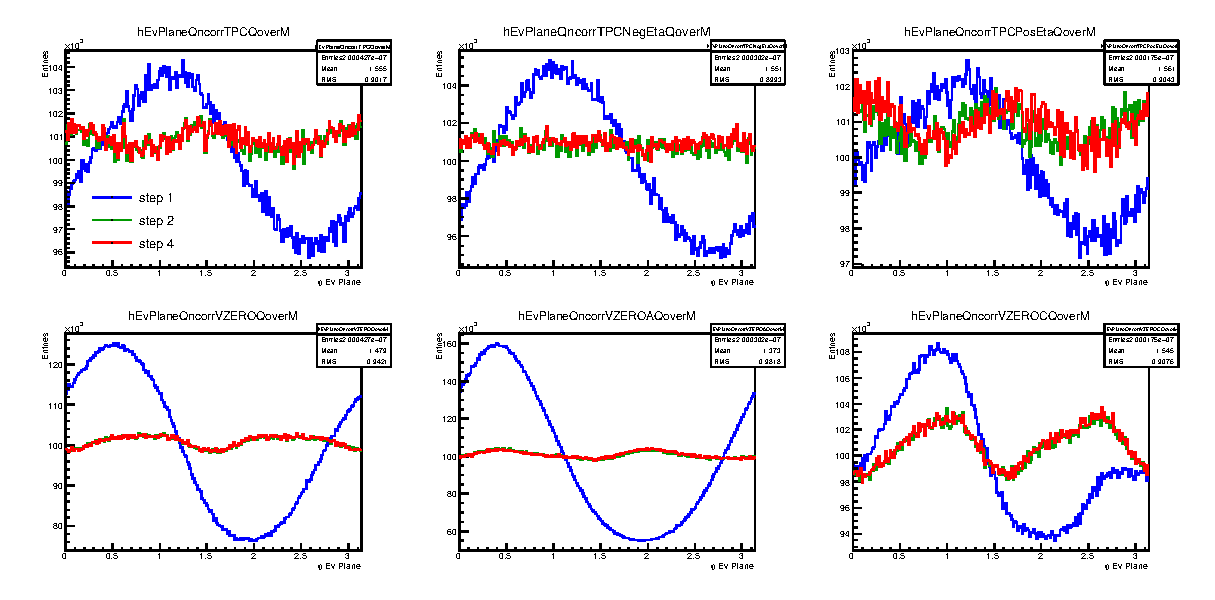
\includegraphics[width=0.9\textwidth]{FigCap5/EP_overMnorm.eps}
 \caption{Event plane distributions obtained with the TPC tracks (top row) and VZERO multiplicity (bottom row) after several stpes of calibration applied using the $Q_n$-correction framework using the $Q/M$ normalization. At step 1 the gain equalization and the
   recentering correction
   information are collected for VZERO and TPC respectively. At
   step 2 the recentering correction is applied to TPC $Q_n$ vector
   and the alignment information are retrieved. For VZERO the gain
   equalization is applied to data and the recentering informations
   collected. At step 4 TPC $Q_n$ vectors are corrected for
   recentering, alignment and twist. VZERO $Q_n$ vectors are corrected
   for gain equalization, recentering
   and alignment.}
   \label{fig:QoverMCalibration}
\end{figure}
\subsection{$v_2$ extraction methods} 

\subsubsection{Method based on invariant mass spectra in 2 bins of $\Delta\phi$} 
\label{epMethodsDescript}
The simplest method used for $v_2$ extraction relies on the 
measurement of the event plane, with either the TPC or the VZERO detectors, as 
explained above and in building the invariant mass distribution of candidates 
in intervals of $\Delta\phi= \phi - \Psi_2$, where $\phi$ is the azimuthal
angle of the $\Dzero$ or $\Dplus$ candidate and $\Psi_2$ is the event plane angle
estimated from the second Fourier harmonic in the azimuthal
distribution of reconstructed particles.
By fitting the invariant mass distributions, the D meson yield can be
measured as a function of $\Delta\phi$. 
The $v_2$ coefficient can then be obtained by fitting the signal yield 
versus $\Delta\phi$ distribution with the following function:
\begin{equation}\label{eq:v2D}
 \frac{dN}{d\phi} = k\cdot(1 + 2v_2\cos(2\Delta\phi))
\end{equation}
where $k$ is a normalization constant. 

%In case of the $\Dstar$-analysis the sample of candidates was divided in 2 or 3 $\Delta\phi$-bins. The number of %$\Delta\phi$-bins depended on the statistical significance $S/\sqrt{S+B}$ of the mass peak in the considered $\pt$-bin. The %$\Dstar$-yield was distributed over the $\Delta\phi$-bins with the requirement that the significance was at least %$S/\sqrt{S+B}=4$ in for each $\Delta\phi$-bin. \\
%In case of the $\Dzero$ and $\Dplus$
In the analysis presented here, the sample of candidates was divided in two $\Delta\phi$ regions: the \textit{in-plane} region and the \textit{out-of-plane} regions. We define the in-plane region (centred on the event plane) as the region $\left(0,\frac{\pi}{4}\right]\cup\left(\frac{3\pi}{4},\pi\right]$ and the out-of-plane as $\left(\frac{\pi}{4},\frac{3\pi}{4}\right]$. Reducing the splitting in $\Delta\phi$ to only two bins allows to improve the statistics for each invariant mass fit. Resolving equation \ref{eq:v2D} for the number of signals measured in the in-plane and out-of-plane regions separately we obtain
\begin{equation}\label{eq:ninout}
 \begin{split}
  & N_\text{in-plane} = k\int_\text{in-plane}1+2v_2\cos(2\phi)d\phi = k'\cdot(\pi+4v_2)\\
  & N_\text{out-plane} = k\int_\text{out-plane}1+2v_2\cos(2\phi)d\phi= k'\cdot(\pi-4v_2)
 \end{split}
\end{equation}
and therefore it is possible to compute $v_2$ from the relative difference between the number of signal observed in-plane and out-of-plane. 
\begin{equation}\label{eq:anis}
 v_2 = \frac{\pi}{4}\frac{N_\text{in-plane}-N_\text{out-plane}}{N_\text{in-plane}+N_\text{out-plane}}
\end{equation}

subsubsection{$\Ds$ azimuthal anisotropy}

The $\Ds$ invariant mass distributions in and out of plane, with the event plane determined by the V0 multiplicity  in the centrality class 30-50\% are shown in Fig. for 5 $p_t$ bins (from 2 to 16 $\GeV/c$).
The fit was performed using a double Gaussian fit to model the $\Ds$ peak and the contribution of the $\DtoKpipi$, BR = (0.277$^{+0.009}_{-0.001}$)\%, which gives rise to a bump in the background shape around 1.870 GeV/c$^{2}$. An exponential shape was also used to model the background.
In Fig., one can also see the comparison of Gaussian pole and sigma for the in/out-of-plane and the $\phi$-integrated yield extraction.
The values of the extracted raw yields and the signal over background for the invariant mass fits in-plane and out-of-plane are reported in table \ref{signalsDs}.

\begin{figure}
\centering
 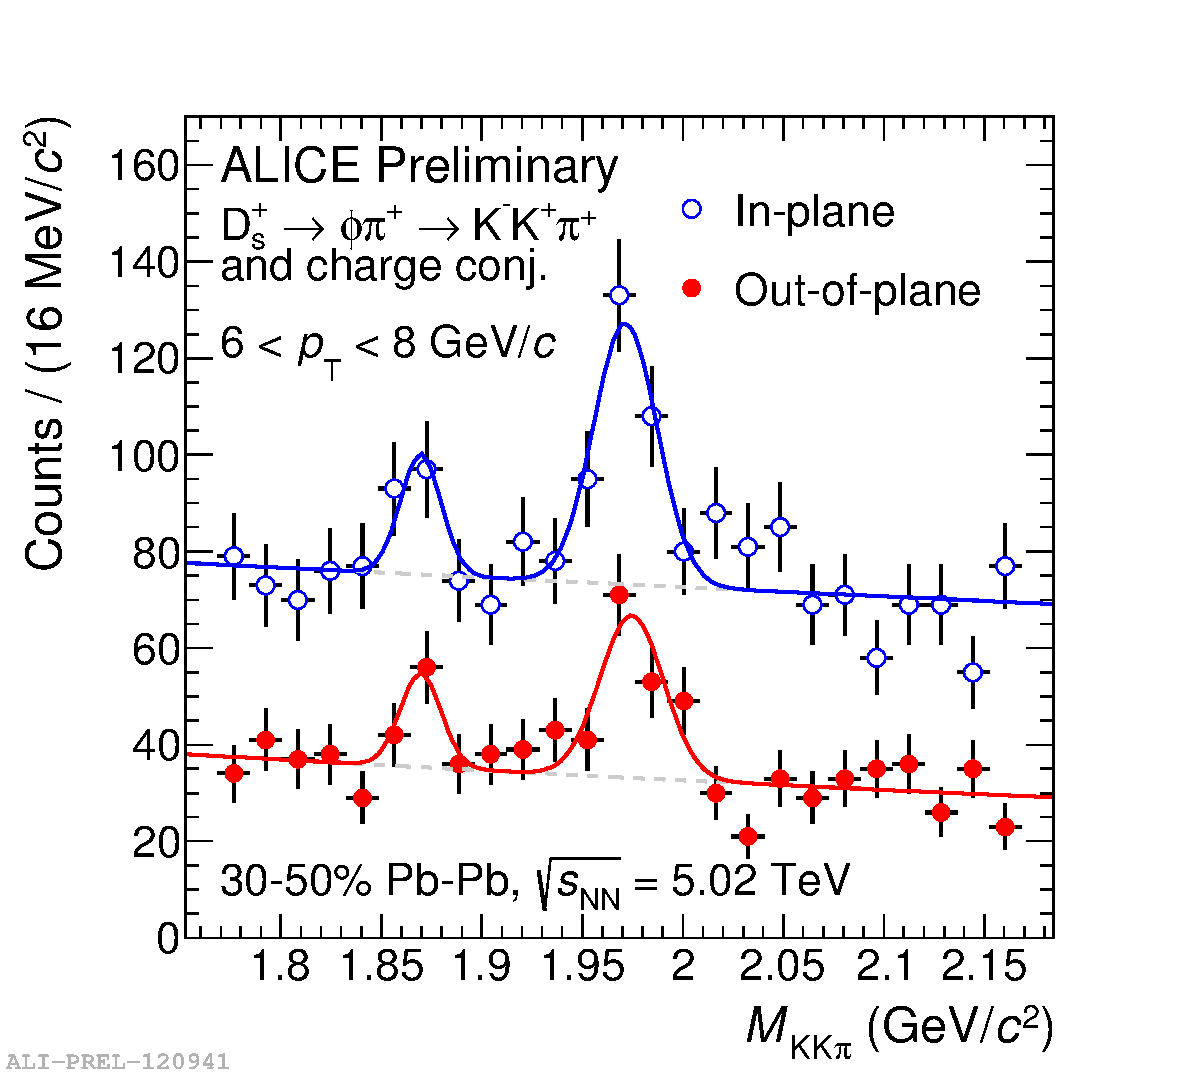
\includegraphics[width=.7\textwidth]{FigCap5/MassDsInOutOfPlane_PbPb3050_5TeV_pt6-8.pdf}
\caption{$\Ds$ invariant mass distribution in the 2 $\Delta\phi$ and 5 $\pt$ intervals.}
\label{fig:2deltaphibinsds}
\end{figure}

\iffalse
\begin{table}[!htbp]
 \caption{$\Ds$,  raw yields and signal over background per $\pt$ bin and $\Delta\phi$ region.}
 \label{signalsDs}
 \begin{center}
  \begin{tabular}{|c|c|c|c|c|}
\hline
\multirow{2}{*} {$\pt$ ($\GeV/c$)}  & \multicolumn{2}{c|}{In-plane} & \multicolumn{2}{c|}{Out-of-plane} \\
\cline{2-5}
& raw yield & S/B & raw yield & S/B\\
\hline
2-4 & $58 \pm 14$ & 0.31 & $34 \pm 11$  & 0.31 \\
\hline
4-6 & $135 \pm 24$  & 0.21 & $97 \pm 18$  & 0.35\\
\hline
6-8 & $134 \pm 21$  & 0.31  & $83 \pm 15$  & 0.43 \\
\hline
8-12 & $70 \pm 11$  & 0.99 & $57 \pm 10$  & 1.36\\
\hline
12-16 & $25 \pm 6$  & 3.00 & $18 \pm 5$  & 1.89 \\
\hline
  \end{tabular}
 \end{center}
\end{table}  
\fi
\section{Systematics}
\label{sec:systematics_010_6080}
The sources of systematic errors considered for the analysis of the D-meson $\RAA$ in 0-10$\%$ and 60-80$\%$ centrality classes are the same as those for the 30-50$\%$ centrality class (see Section ?). In particular, the main sources are:
\begin{enumerate}
\item Systematic uncertainty due to the raw-yield extraction.
\item Systematic uncertainty due to the topological selection efficiency.
\item Systematic uncertainty due to the PID selection efficiency.
\item Systematic uncertainty due to the generated $\pt$ shape of the D mesons for the efficiency computation.
\item Systematic uncertainty due to the tracking efficiency.
\item Systematic uncertainty due to the beauty feed-down subtraction.
\end{enumerate}

\subsection{Raw-yield extraction}
To estimate the systematic uncertainty due to the raw-yield extraction, a multi-trial approach was used. The description of this strategy was reported in Section ?.
The results for the $\Dplus$ are shown in Fig. for the 0-10$\%$ centrality class and in Fig. for the 60-80$\%$ centrality class. The left panel shows the raw yield (and its statistical uncertainty) as a function of the number of trial. In the first half of the trials the sigma of the Gaussian function was let free in the fit, while in the second half fixed to the value obtained by fitting the singal in the MC simulation. The blue histograms display the results from the fitting approach, while the green and orange histograms those from the bin-counting method. The right panel shows the distribution of the raw yield from the various trials. The red line corresponds to the raw yield used for the central value of the measurements. In most of the cases it falls in the center of the raw-yield distributions. The largest uncertainty is observed for the first four $\pt$ intervals in the 0--10$\%$ centrality class. This is mainly due to the large amount of combinatorial background and therefore the small signal over background ratio. In particular, it is possible to observe several trials for which the value of the raw yield varies significantly, and then it remains almost flat: these points correspond to those trials for which a different fit function for the background is used (exponential, linear and second order polinomial). In the interval $4<\pt<5$ $\GeV/c$ several trials are missing because the reduced chi square of the fit was larger than 2, and therefore they were rejected. Most of these fits were performed using the linear fit function to describe the combinatorial background. At intermediate $\pt$ the variation of the raw yields decreases, reaching a minimum of about $2\%$ in the $4<\pt<5$ $\GeV/c$ interval for the 60--80$\%$ centrality class. For the $\Ds$ meson, the results are presented in Fig..
The approach is essentially the same as that described above for the $\Dplus$ meson. The panels show, starting from the top left:
(i) the raw yield distribution from multiple trials, when using signal extraction from fit procedure and from bin counting method, in different colours; (ii) distribution of raw yields from multiple trials, distinguishing the cases of Gaussian sigma left as free parameter in the fit, fixed to MC value and fixed to MC value $\pm$ 15\%; (iii) the $\chi^{2}$ distribution for the extracted yields; (iv) the sigma of the Gaussian fit as a function of the number of trials; (v) the raw yield distribution as a function of the number of trial; (vi) since the systematic is estimated from the RMS value of the yield distribution, in the panel the ratio of the 
RMS over the mean of the distribution is reported for three cases: considering the fits with all the values for the sigma (free, fixed to MC, fixed to MC $\pm$ 15\%), considering the fits with sigma free, fixed to MC, fixed to MC $+$ 15\% or with sigma  free, fixed to MC, fixed to MC $-$ 15\%. 
In this way, for those $\pt$ intervals where the values of the free sigma were on average displaced towards values of sigma MC $+ (-)$ 15\%, the
second (third) value of the RMS was chosen to give the final systematics. In the assigned systematic uncertainty, it was verified that the
systematics from the bin counting method is contained in the quoted number.

The numerical values of the systematic uncertainty due to the yield extraction, determined bin by bin for all the three non-strange D mesons are shown in Table, while in in Table for the $\Ds$ meson.



\begin{figure}[!htb]
 \begin{center}
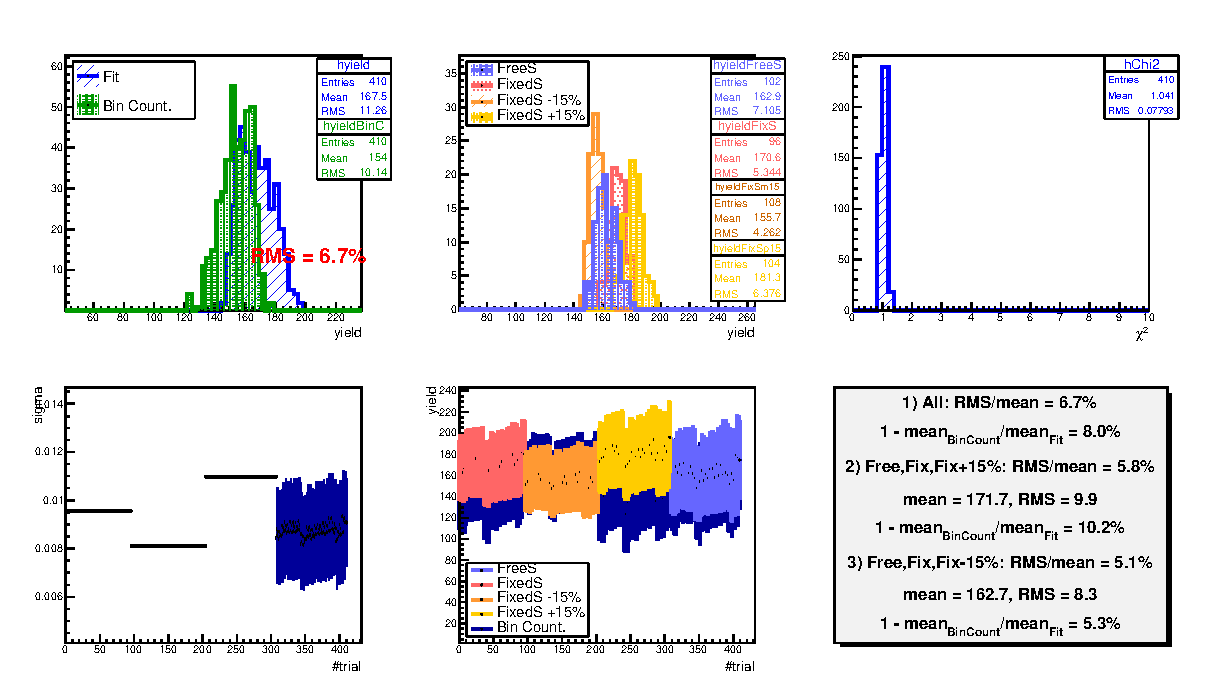
\includegraphics[angle=0, width=10.cm]{./FigCap5/MT_Pt46_010.eps}
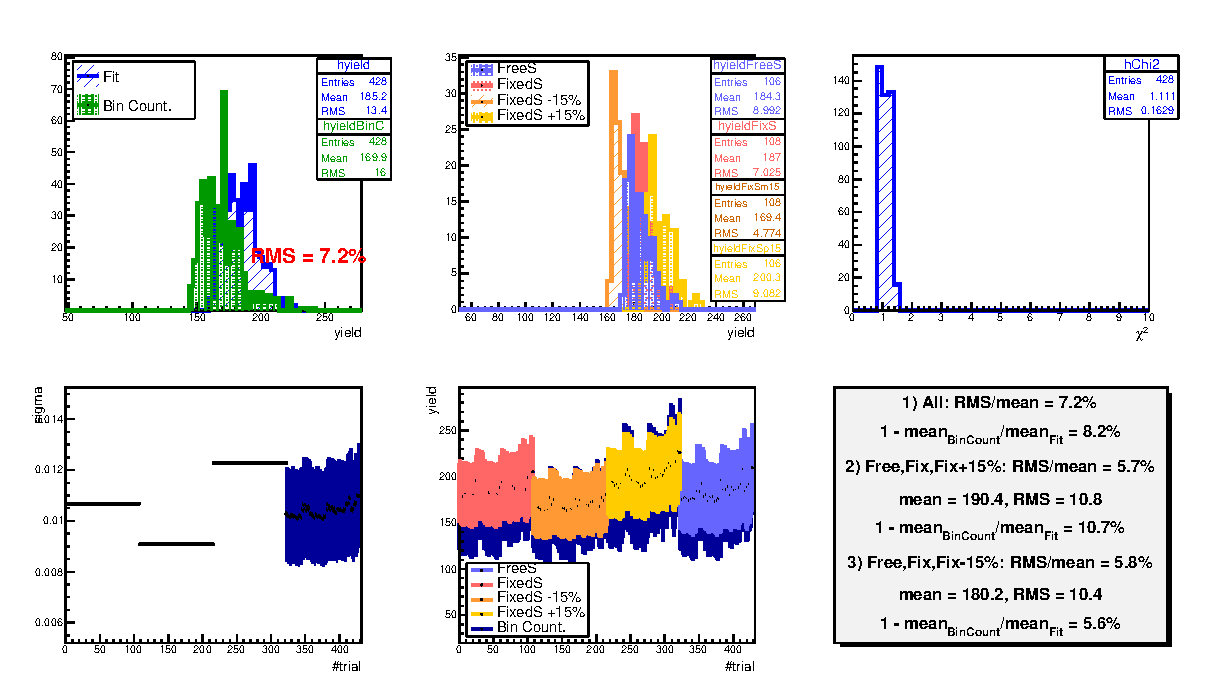
\includegraphics[angle=0, width=10.cm]{./FigCap5/MT_Pt68_010.eps}
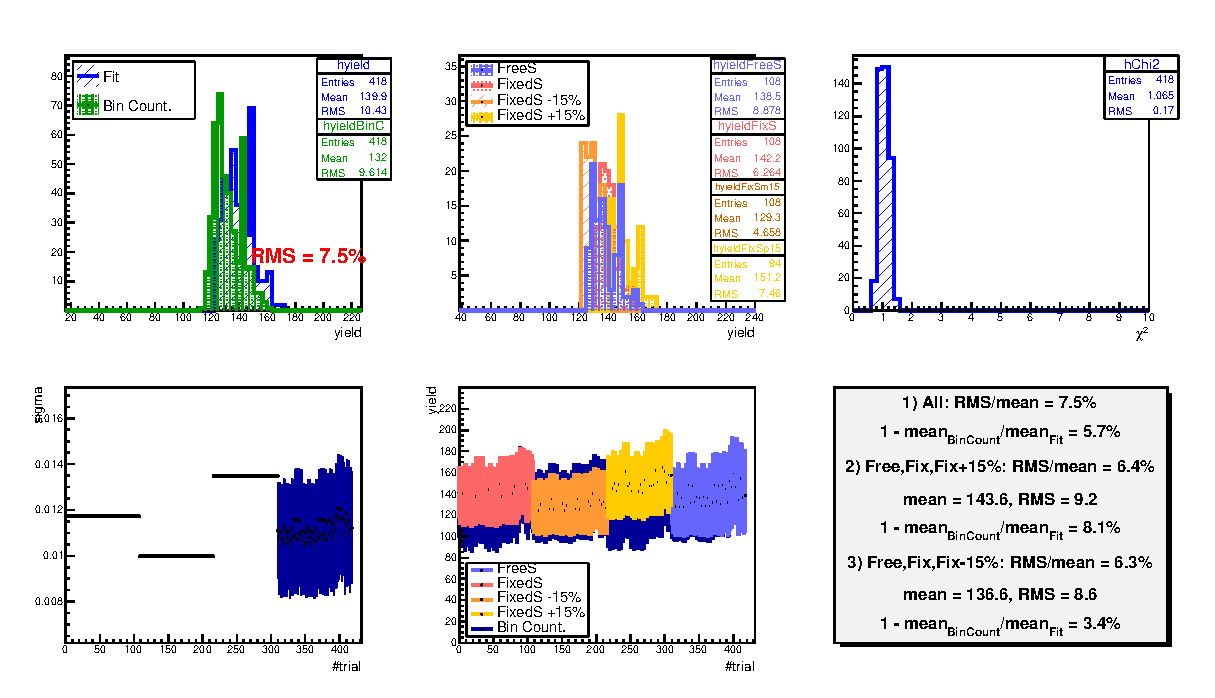
\includegraphics[angle=0, width=10.cm]{./FigCap5/MT_Pt812_010.eps}
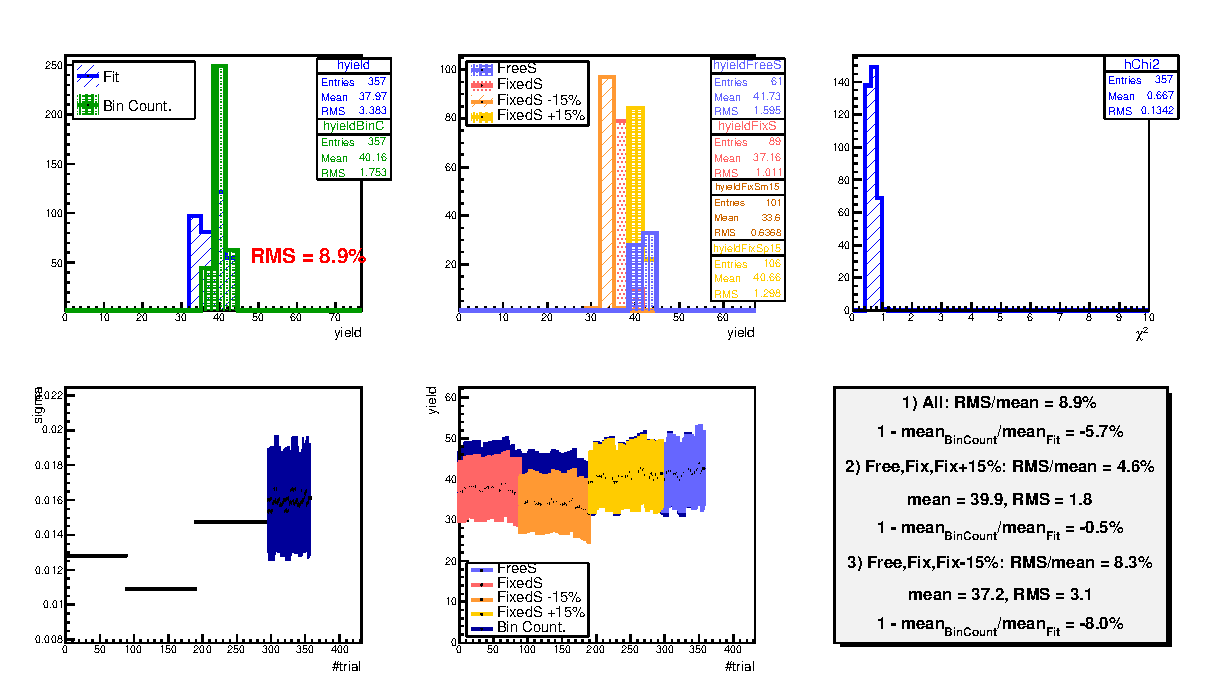
\includegraphics[angle=0, width=10.cm]{./FigCap5/MT_Pt1216_010.eps}
\end{center}
 \caption{Output of multi-trial fits to $\Ds$ invariant mass distributions in the $\pt$ intervals 4-6, 6-8, 8-12, 12-16 $\GeV/c$  for the 0-10$\%$ centrality class.}
 \label{multitrial_Ds_010}
\end{figure}

\begin{figure}[!htb]
 \begin{center}
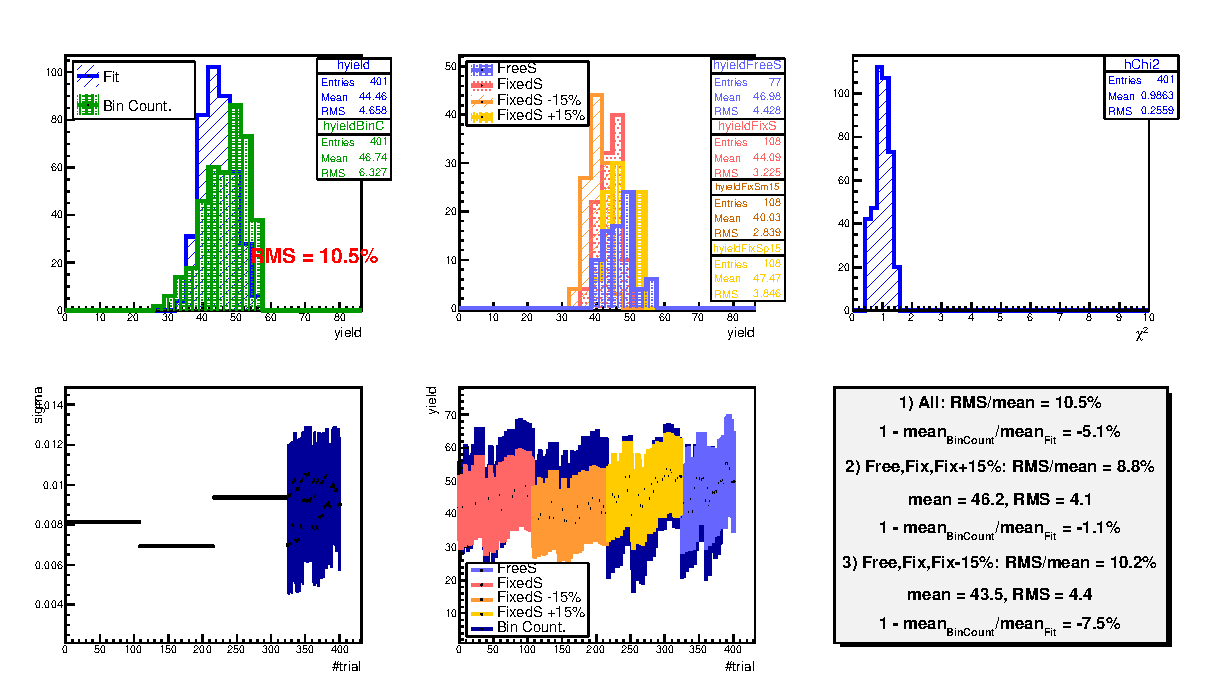
\includegraphics[angle=0, width=8.cm]{./FigCap5/MT_Pt24_6080.eps}
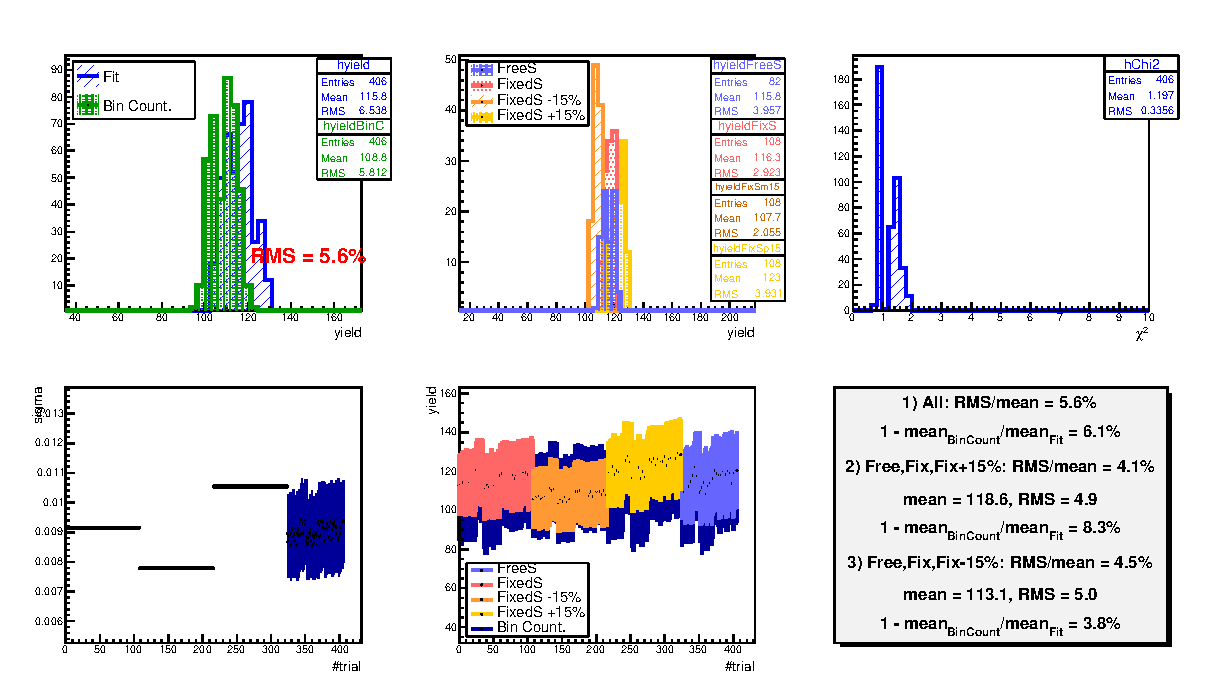
\includegraphics[angle=0, width=8.cm]{./FigCap5/MT_Pt46_6080.eps}
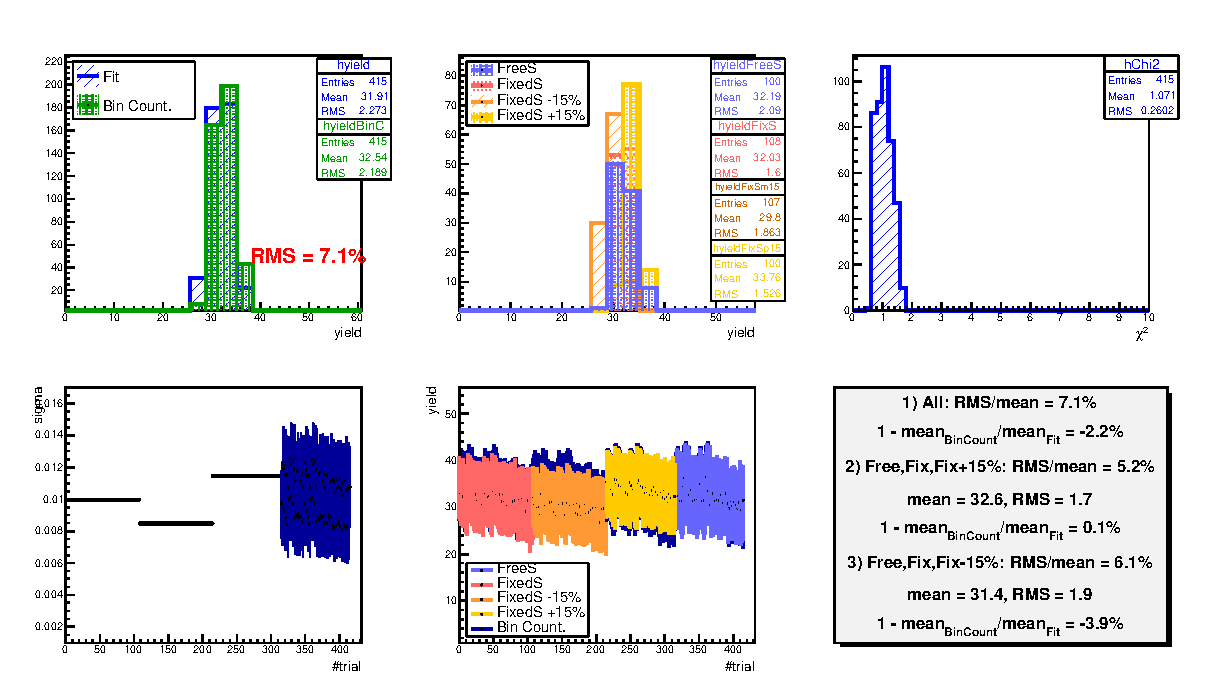
\includegraphics[angle=0, width=8.cm]{./FigCap5/MT_Pt68_6080.eps}
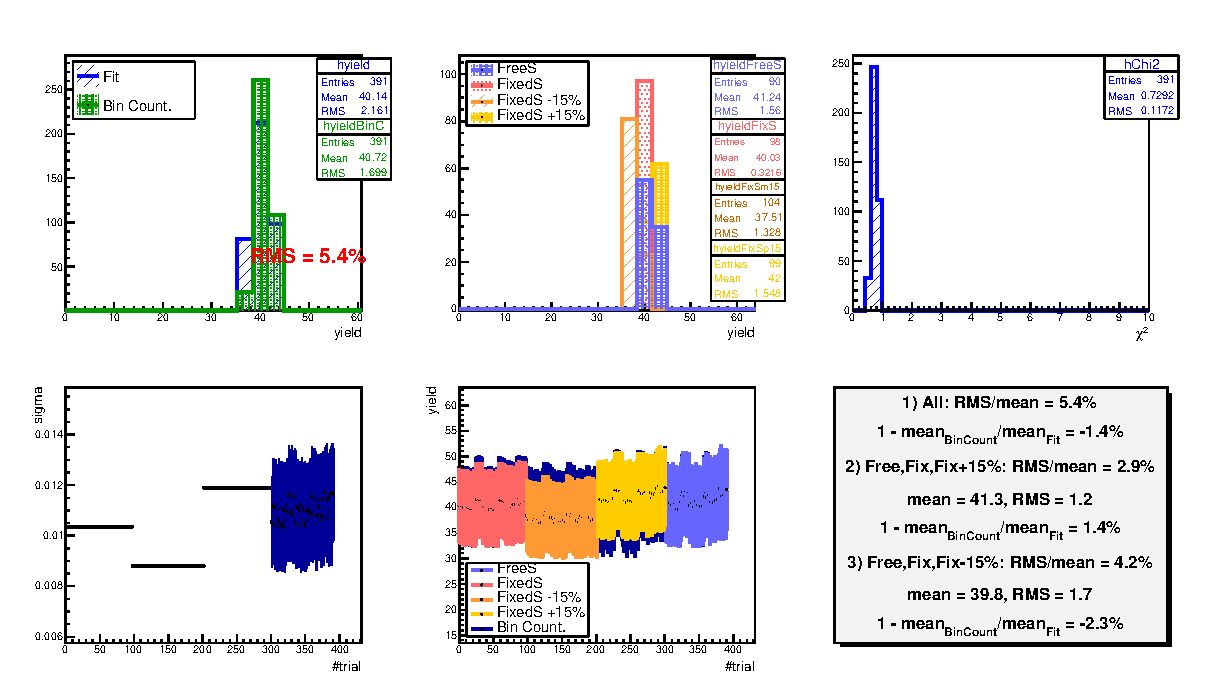
\includegraphics[angle=0, width=8.cm]{./FigCap5/MT_Pt812_6080.eps}
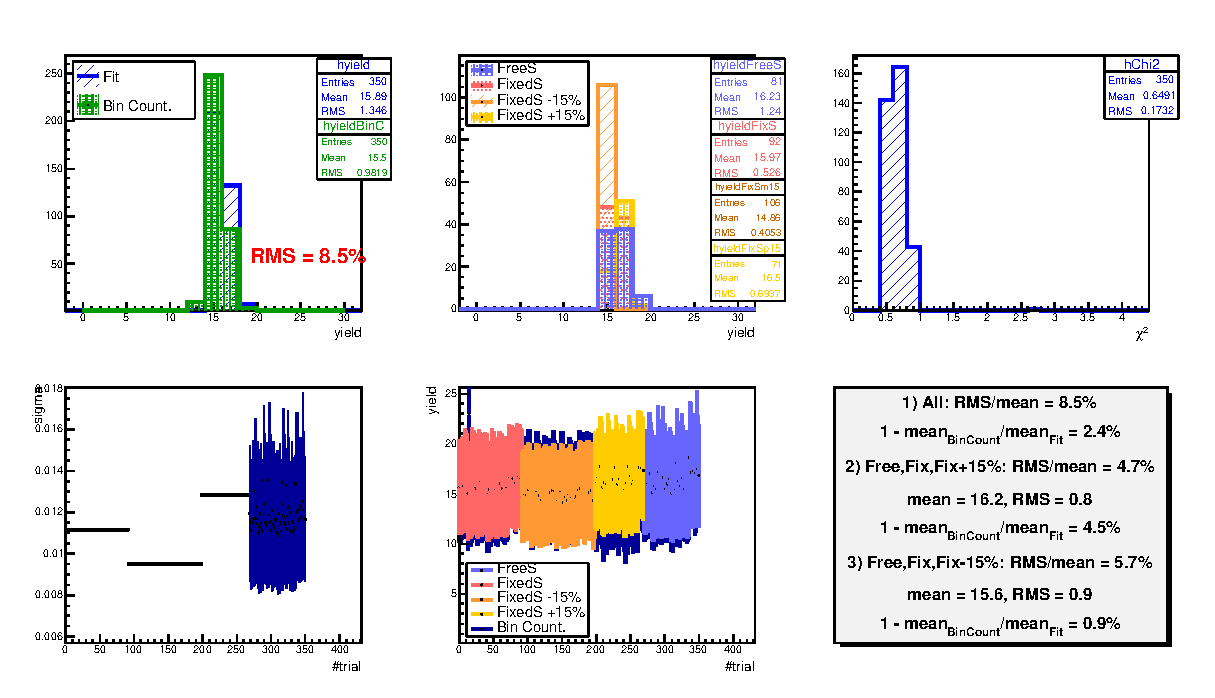
\includegraphics[angle=0, width=8.cm]{./FigCap5/MT_Pt1216_6080.eps}
\end{center}
 \caption{Output of multi-trial fits to $\Ds$ invariant mass distributions in the $\pt$ intervals 2-4, 4-6, 6-8, 8-12, 12-16 $\GeV/c$  for the 60--80$\%$ centrality class.}
 \label{multitrial_Ds_6080}
\end{figure}




\subsubsection{Topological selection efficiency}
For the $\Ds$ meson, it was repeated the approach already described in Section  for the
30--50\% centrality class, when a scan over each topological variable used in the selection was performed,
looking for possible trends in the corrected yields. With a careful study of each extraction, meant to exclude those cases
where the yield extraction is not stable enough, all the corrected yields were then collected into final distributions (Fig.~\ref{DsCutVar_010} and~\ref{DsCutVar_6080}) for each 
$\pt$ interval, that are used to provide the RMS values for the systematic uncertainty estimate. In general, since
the corrected yield distribution is quite Gaussian, the systematics come form the Gaussian RMS; for the $\pt$
intervals 6-8 and 8-12 GeV/c in the 60--80\% centrality class, the RMS was calculated as full spread divided by $\sqrt{12}$,
since the yield distribution has some tails deriving from the scan over NDLxy variable.
\begin{figure}[!ht]
 \begin{center}
   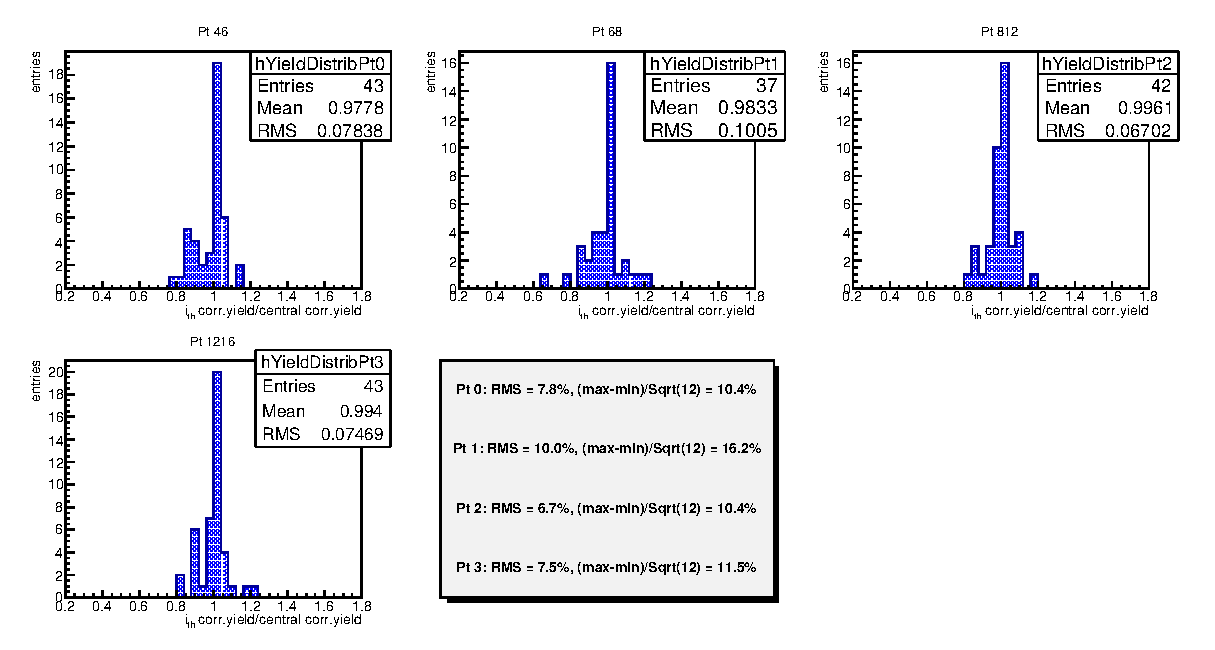
\includegraphics[angle=0, width=15cm]{./FigCap5/FinalSyst_010.eps}
 \end{center}
 \caption{Distribution of $\Ds$ corrected yields in the 0-10\% centrality class, obtained varying the selection on the topological variables with respect to the default value.}
 \label{DsCutVar_010} 
\end{figure}

\begin{figure}[!ht]
\begin{center}
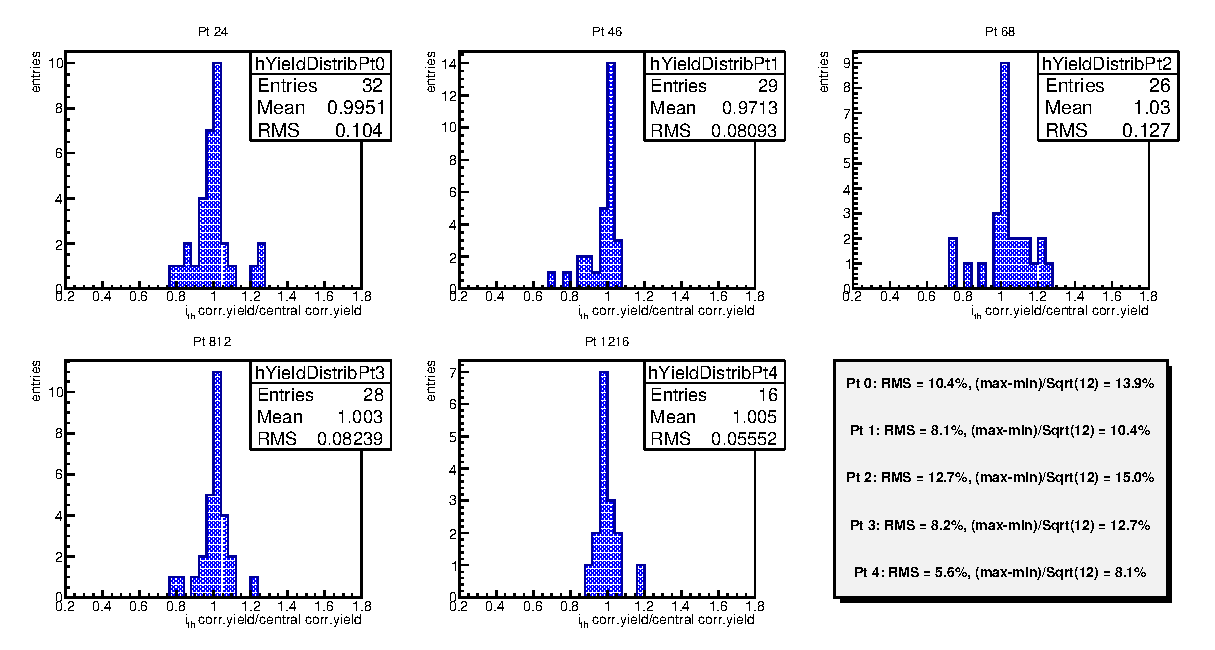
\includegraphics[angle=0, width=15cm]{./FigCap5/FinalSyst_6080.eps}
\end{center}
\caption{Distribution of $\Ds$ corrected yields in the 60-80\% centrality class, obtained varying the selection on the topological variables with respect to the default value.}
\label{DsCutVar_6080} 
\end{figure}

\subsection{PID selection efficiency}

Usually, in the D-meson analysis, the systematic error on the PID is evaluated through the comparison of the
corrected yield obtained with and without applying the PID. In the $\Ds$ case, the rare signal and the large
background do not allow for a signal extraction without particle identification at low $\pt$. The PID cut used
for $\Ds$ for $\pt < $6 GeV/c (namely strong PID) was hence compared to the standard one used at high $\pt$ and for the non-strange D
mesons (namely conservative PID). In Fig. it is shown the ratio of the corrected yield obtained with
conservative PID and the one obtained with the strong one, using the reference set of cuts.
As one can see from the plot, fluctuations of the order of 15-20\% are observed for the central events up to $\pt < 12$ GeV/c.
Since it is very difficult to asses about the extent of contribution from real biases in PID efficiency inside the 15-20\% observed variation 
and hence to disentangle them from statistical fluctuations originating from yield extraction, an alternative approach of a per-track systematic was tried.
The idea is to compare the N-sigma cut efficiency in data and MC for pions and kaons in TPC and TOF, and to propagate then the
assigned per-track systematic to the D-meson candidate level, through the daughter's kinematics.
While for the simulated pions and kaons it is enough to select for the PDG code of the particle, on data one has to clean 
the sample in order to have a consistent comparison. Pions from V0 decays were selected using the already optimised selection
implemented in the AliESDv0KineCuts class. In Fig.~\ref{MCPionsTPC} the Monte Carlo N-sigma distribution for the pion dE/dx in TPC are shown.
The distribution for all the pions in the ESD event requiring the PDG code (in green) is compared to the
distributions of pions passing the optimised selection for V0 decays (in red and blue respectively with and without PDG code selection).
From this comparison, we conclude that the selection of pions from V0 cleans enough the sample and is safe to be applied 
on data for our purposes. Since a second population on the right of the peak is visible at low $\pt$, for the distributions
of pions passing the V0 selection, only the left region of the peak is used to evaluate the systematics.
In Fig. the comparison of the distribution in data (red) is compared
with the same MC distribution in blue and green from Fig.. Both of them are used to calculate
the final systematics. In Fig. the same distributions are shown for the pion time-of-flight signal.
Finally, to identify a sample of kaons in the TPC, a tight cut requiring N sigma $< 0.25$ from kaon hypothesis for the TOF
signal was required. The obtained distribution (black curve in Fig.), was then fitted with a Gaussian to extrapolate the
kaon contribution. The ranges of the fit are set, for each $\pt$ interval, in the region less affected by other species contribution.
In Fig.~\ref{DataKaonsTPC} the distribution for data in the TPC obtained cutting at N sigma $< 0.25$ from kaon hypothesis 
for the TOF signal are shown. The yellow Monte Carlo template for true kaons is superimposed to the data distribution, 
only for visualisation purposes, and not used in the fit. The values of the final systematics, obtained as the ratio
of the efficiencies in data and MC as a function of $\pt$, cutting at 1, 2, 3 sigmas in the distributions with respect to a
cut at 5 sigmas, are shown in Fig.. 
It was verified that enlarging the number of sigmas from 5 to 10 at the denominator does not affect the results.
Since systematics for pions and kaons in TPC show similare values, an assumption was made for
systematics for kaons in TOF to be similar to those of pions in TOF. These values were then propagated 
with the $\Ds$' daughters kinematics, keeping into account the cuts used within the strong PID selection.
 The values of the PID systematics for the $\Ds$ are shown in Fig. and are around a 3\% value.
 Similar results were obtained calculating efficiencies for Monte Carlo using the distribution obtained with
 the PDG selection code or without it.
\begin{figure}[!h]
 \centering
 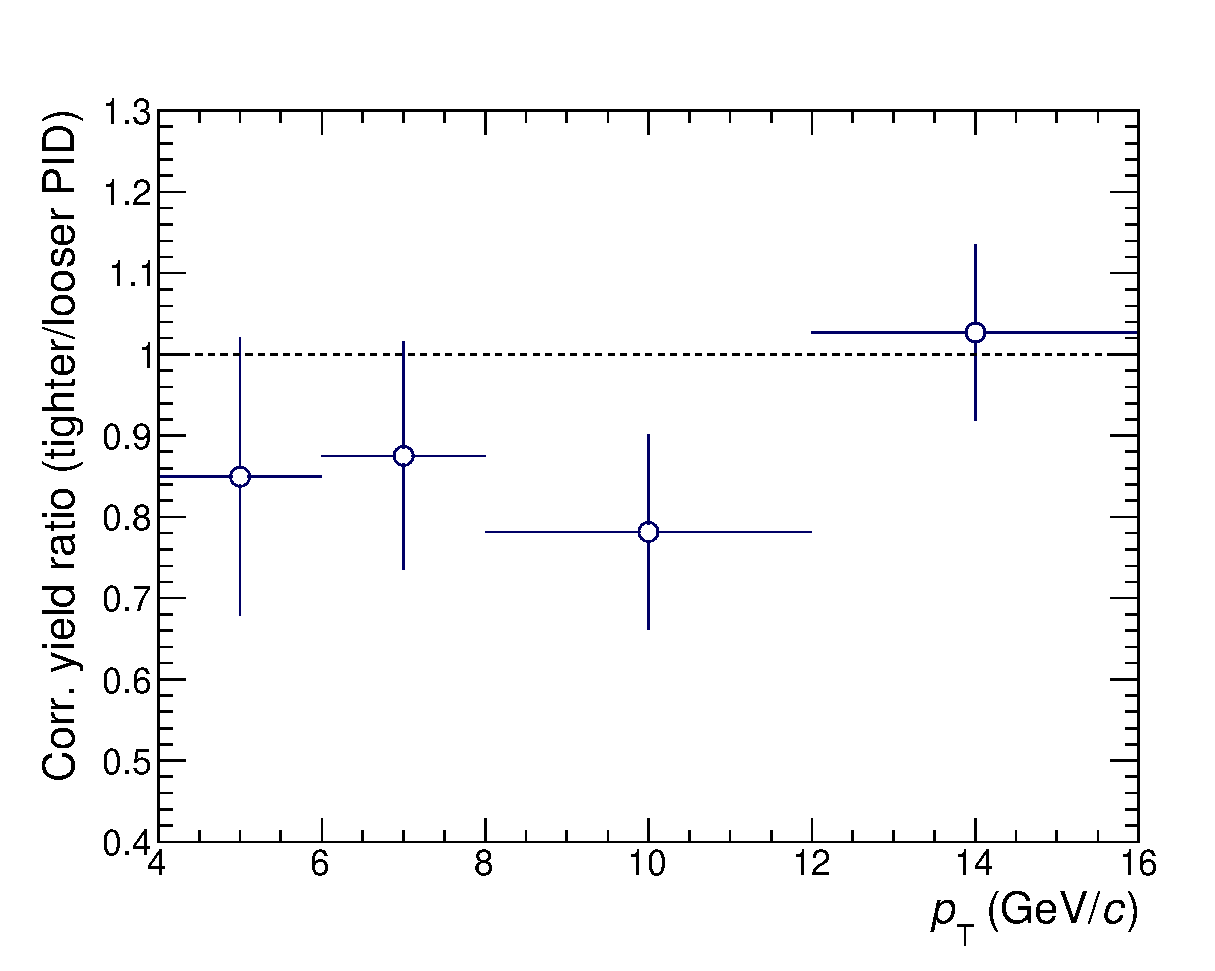
\includegraphics[angle=0, width=7cm]{./FigCap5/PIDsyst_010.eps}
 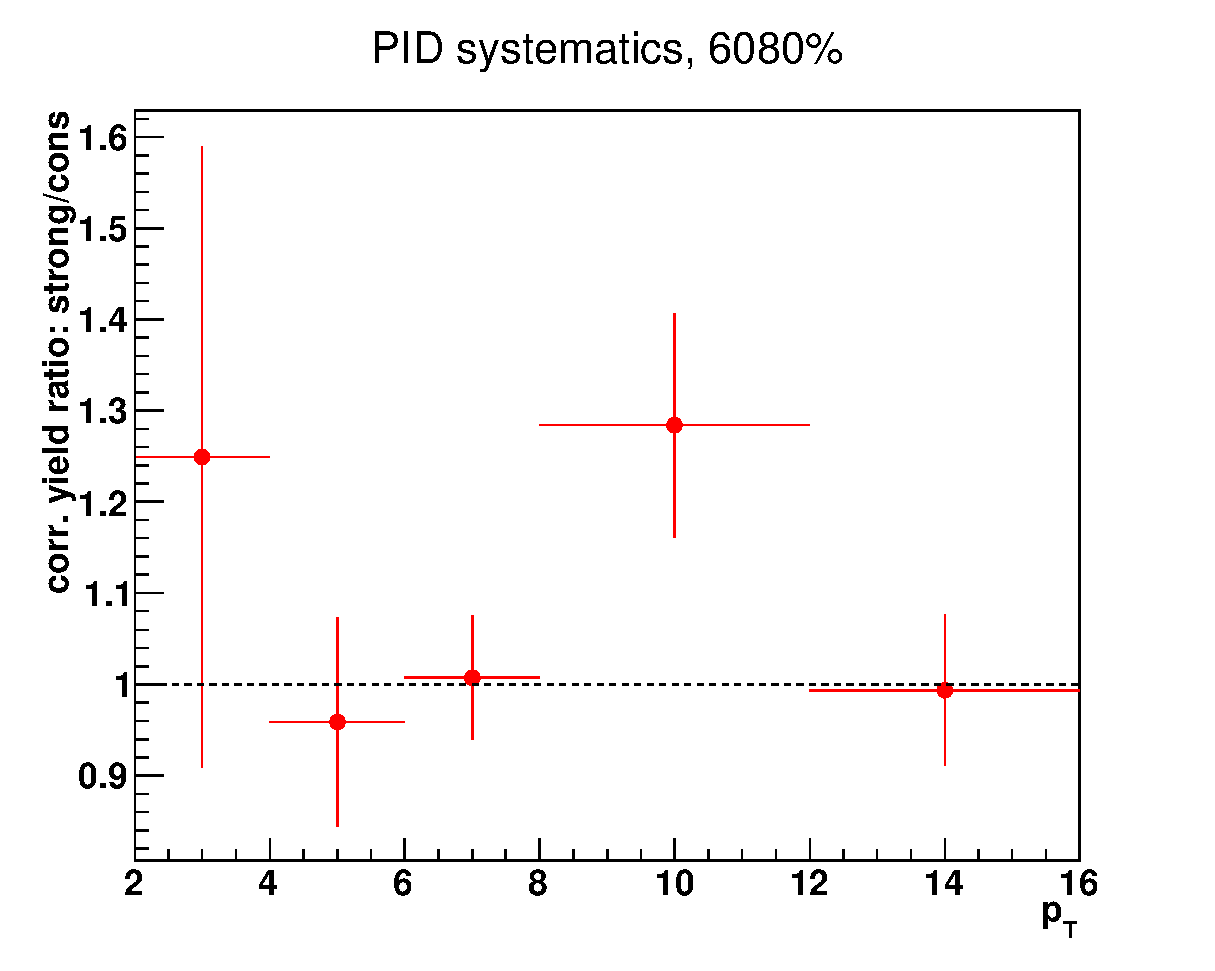
\includegraphics[angle=0, width=7cm]{./FigCap5/PIDsyst_6080.eps}
 \caption{Ratio of $\Ds$ corrected yield in 0--10\% (left) and 60--80\% (right) centrality classes when using strong and conservative PID selections.}
 \label{fig:DsPID0106080} 
\end{figure}

\begin{figure}[!h]
 \centering
 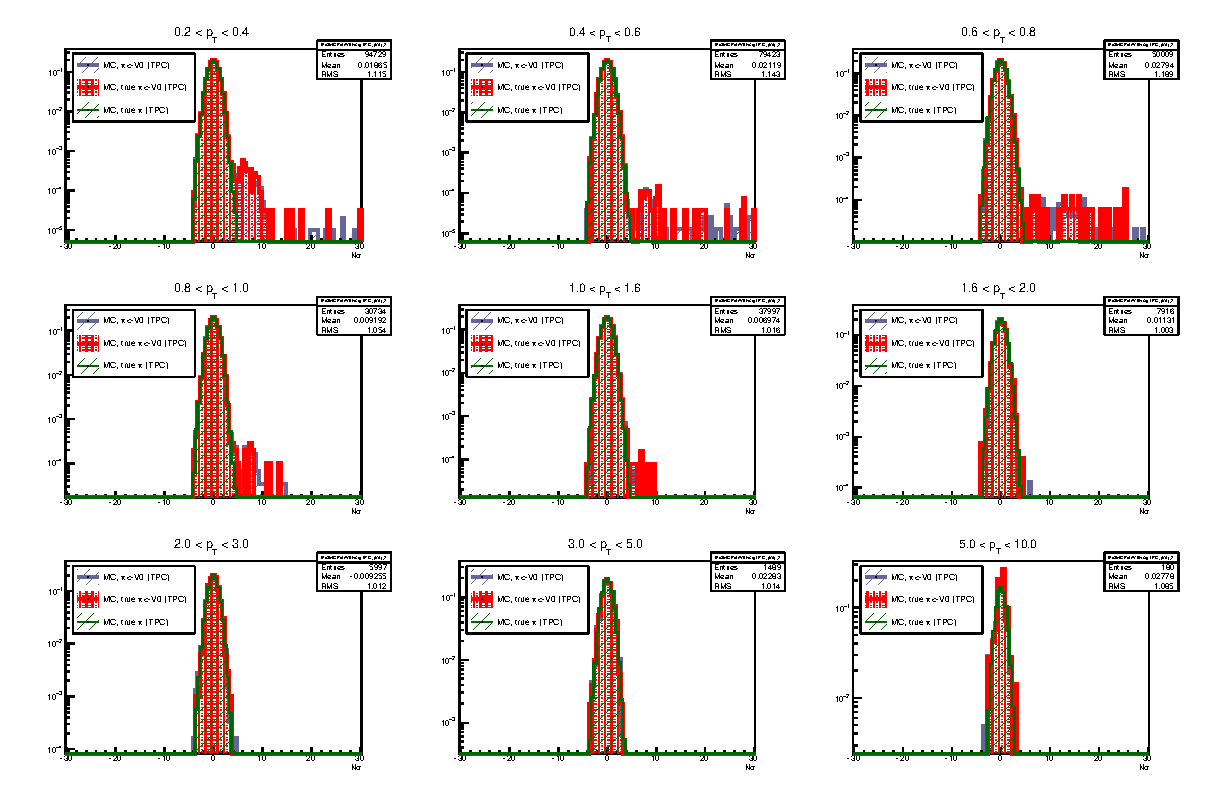
\includegraphics[angle=0, width=13cm]{./FigCap5/MCPionTPC_AllTrueSig.eps}
 \caption{N-sigma distribution for dE/dx signal in TPC from pion hypothesis in Monte Carlo. In green pions selected by PDG code, in blue and in red pions passing the selection for V0 decays without and with PDG code selection respectively.}
 \label{fig:MCPionsTPC} 
\end{figure}

\begin{figure}[!h]
 \centering
 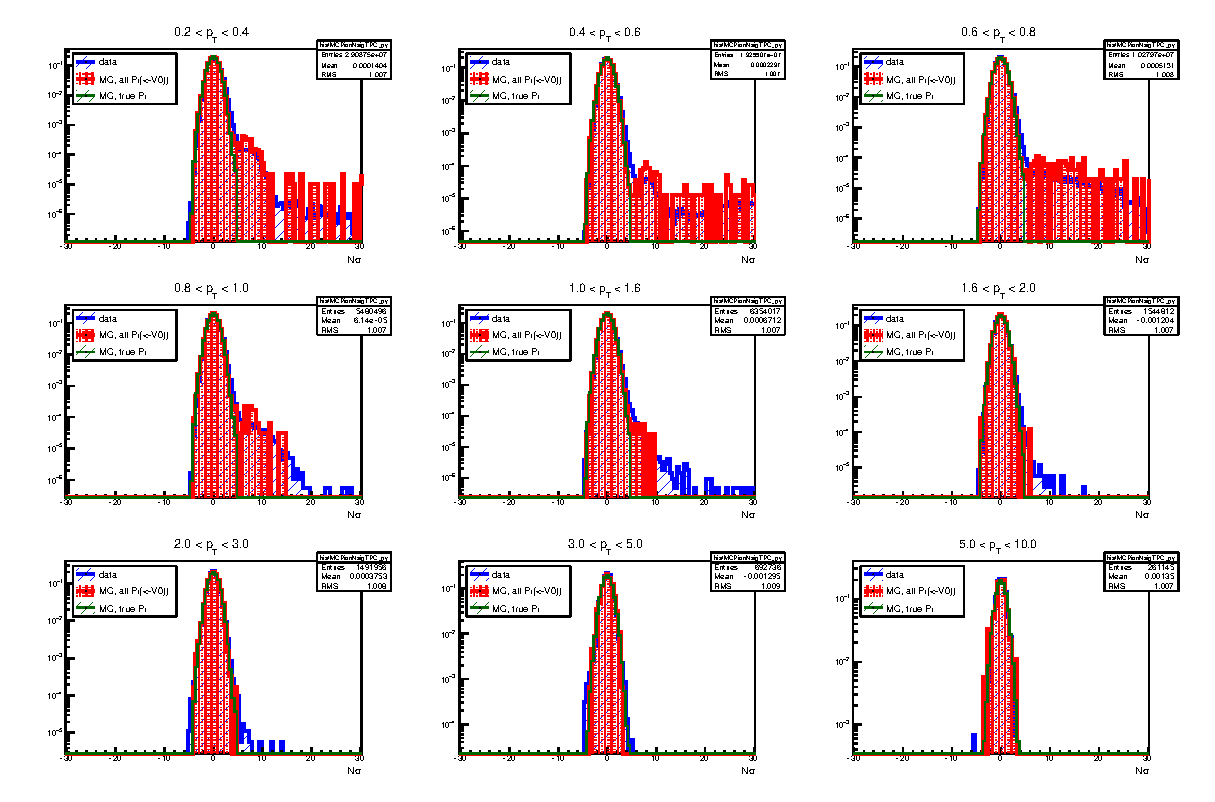
\includegraphics[angle=0, width=13cm]{./FigCap5/PionTPC_DataMC.eps}
 \caption{N-sigma distribution for dE/dx signal in TPC from pion hypothesis in data and Monte Carlo. In green pions selected by PDG code, in blue and red pions passing the selection for V0 decays in Monte Carlo and data respectively.}
 \label{fig:DataPionsTPC} 
\end{figure}

\begin{figure}[!h]
 \centering
 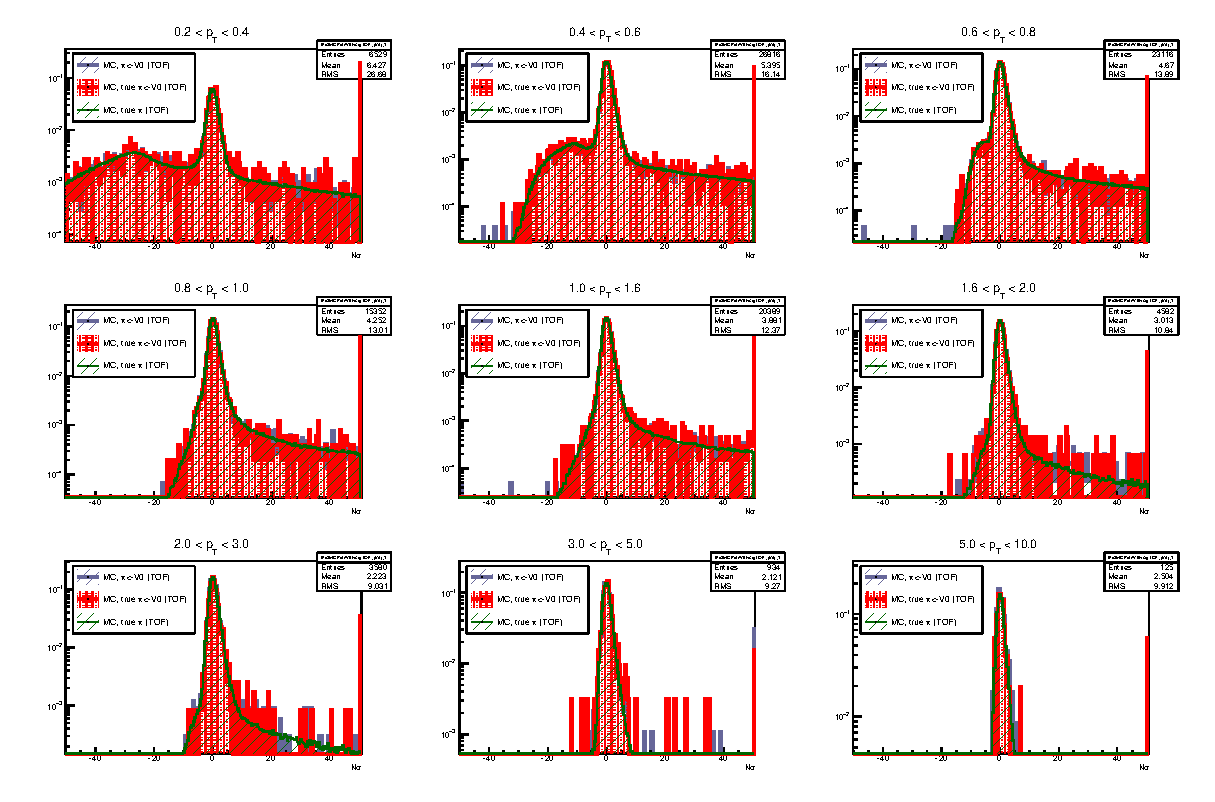
\includegraphics[angle=0, width=13cm]{./FigCap5/MCPionTOF_AllTrueSig.eps}
 \caption{N-sigma distribution for t.o.f. signal in TOF from pion hypothesis in Monte Carlo. In green pions selected by PDG code, in blue and in red pions passing the selection for V0 decays without and with PDG code selection respectively.}
 \label{fig:MCPionsTOF} 
\end{figure}

\begin{figure}[!h]
 \centering
 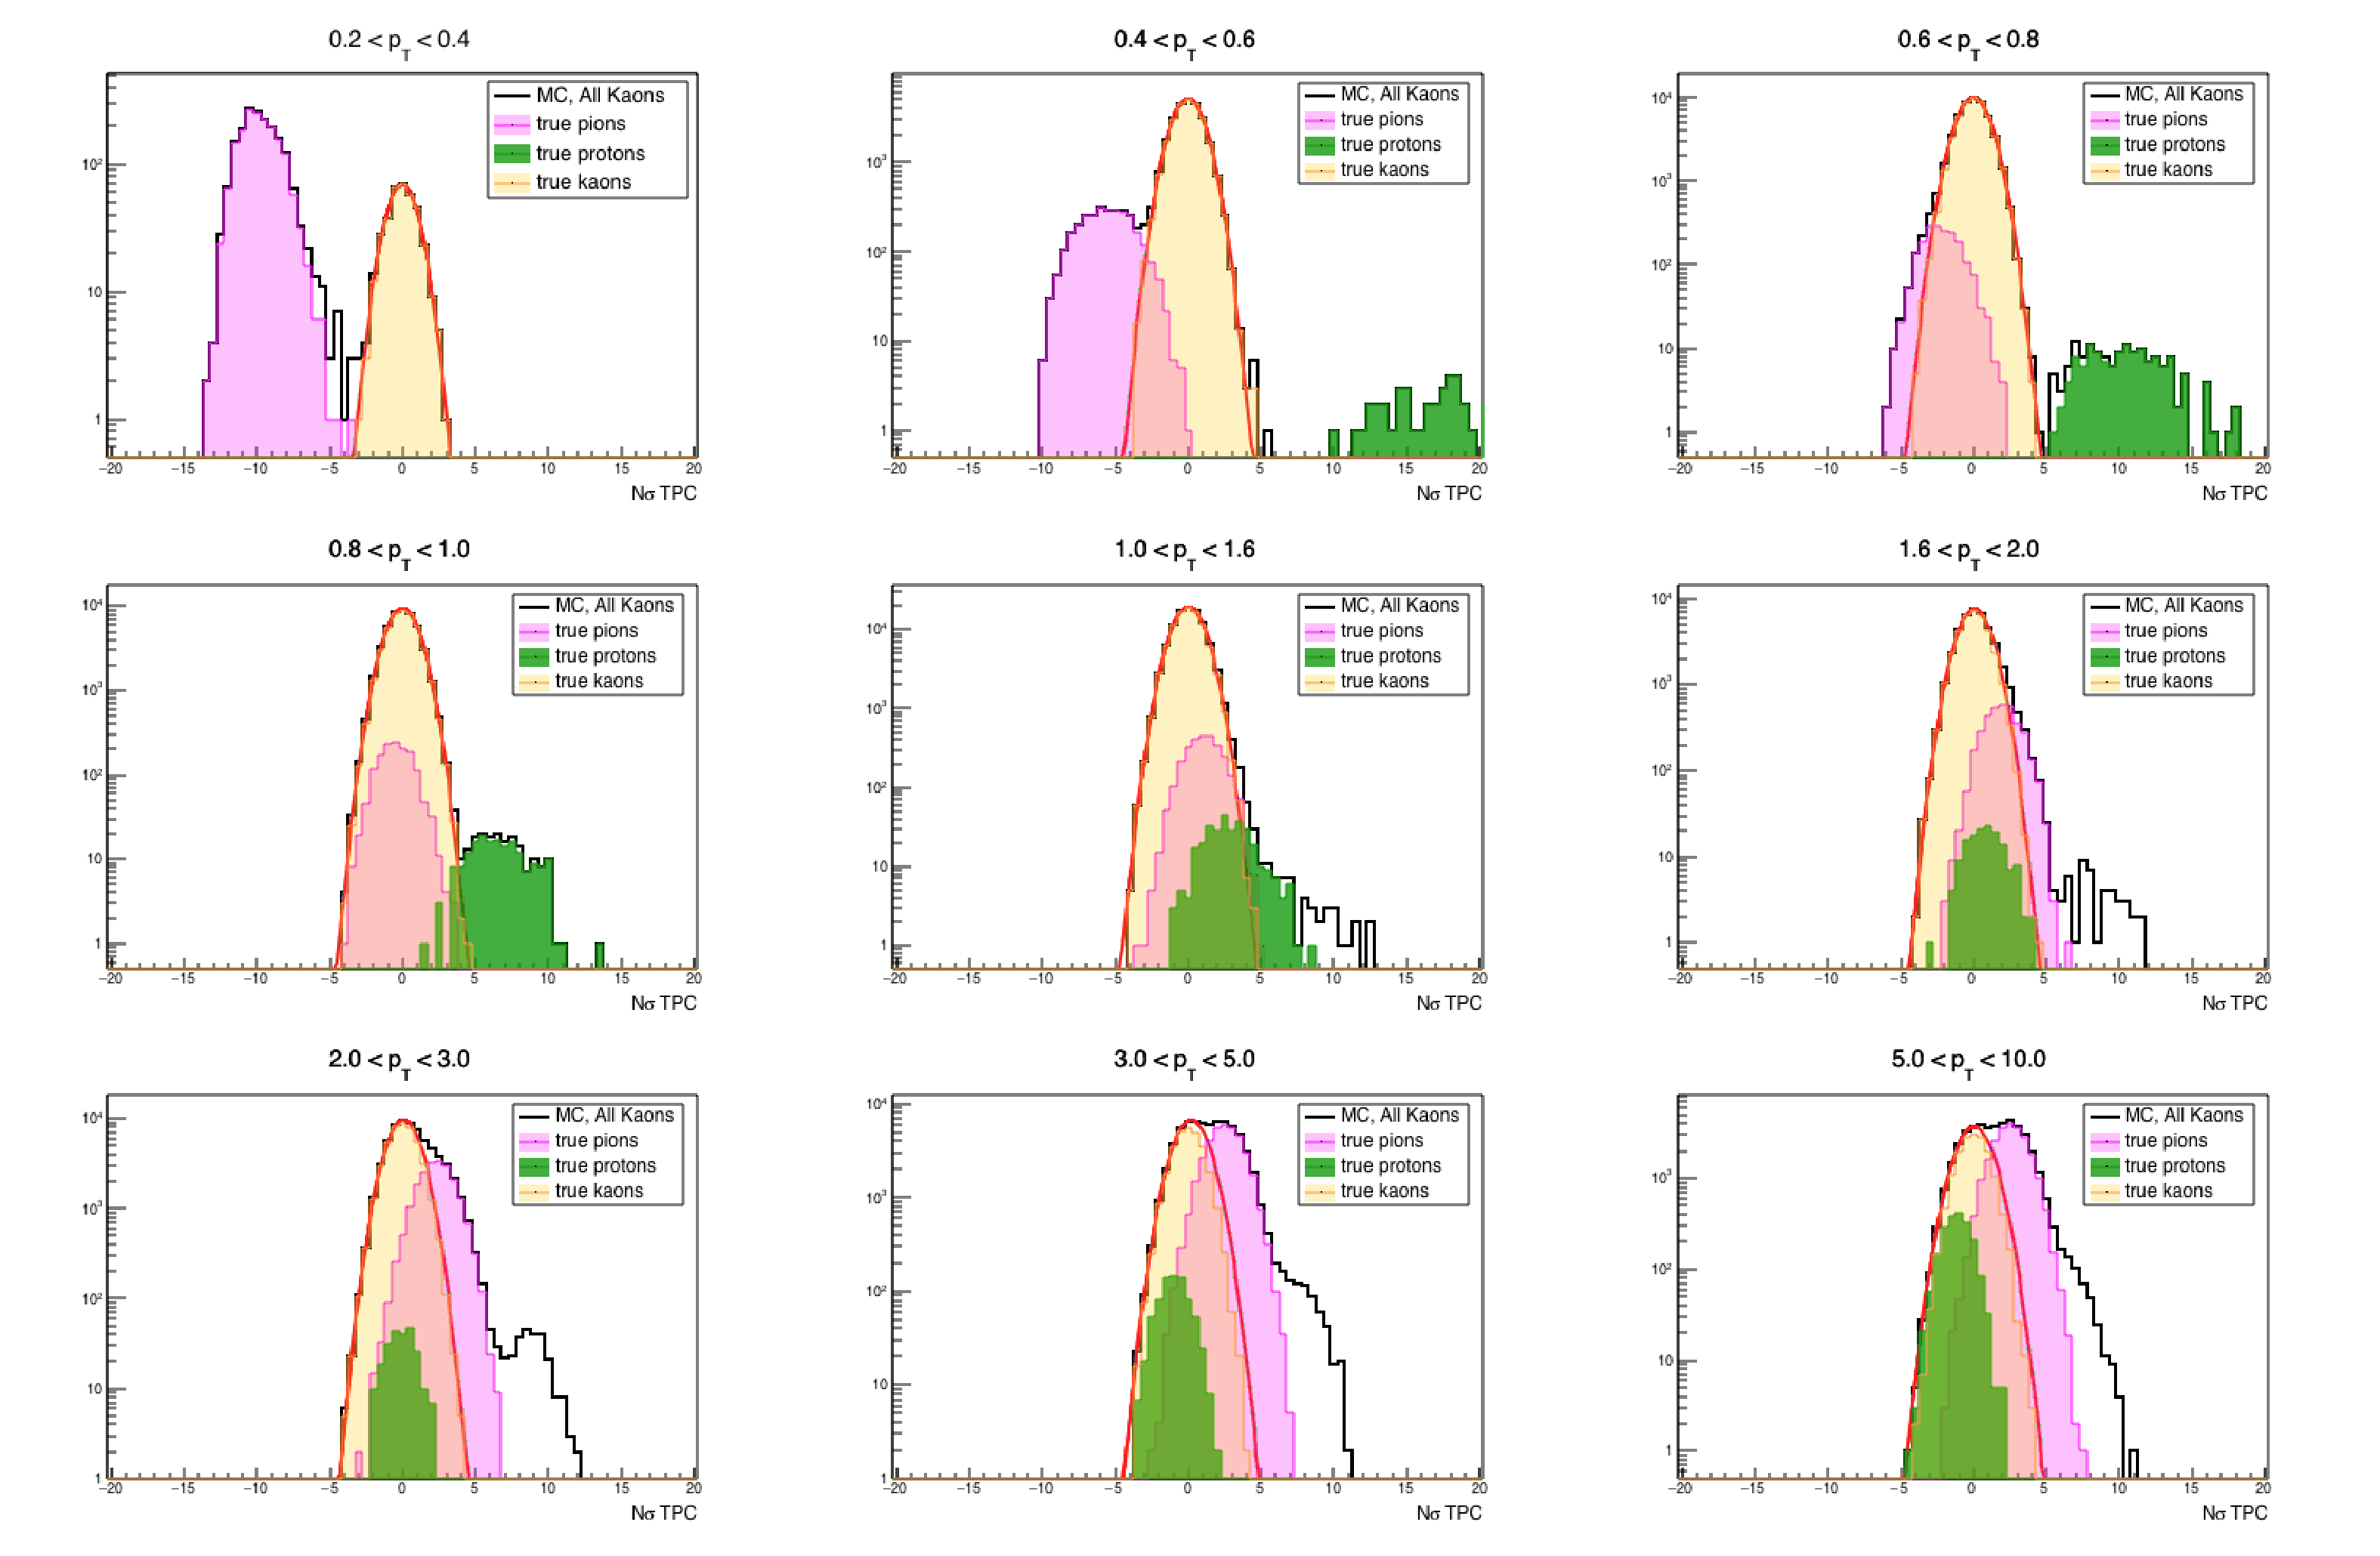
\includegraphics[angle=0, width=13cm]{./FigCap5/MCKaonComponents.eps}
 \caption{N-sigma distribution for dE/dx signal in TPC from kaon hypothesis in Monte Carlo, after a cut at sigma $<$ 0.25 from kaon hypothesis for TOF signal. In yellow, contribution from true kaons, in magenta from pions and in green from protons. In red, the fit to extrapolate the kaon component in the inclusive distribution.}
 \label{fig:DataPionsTOF} 
\end{figure}

\begin{figure}[!h]
 \centering
 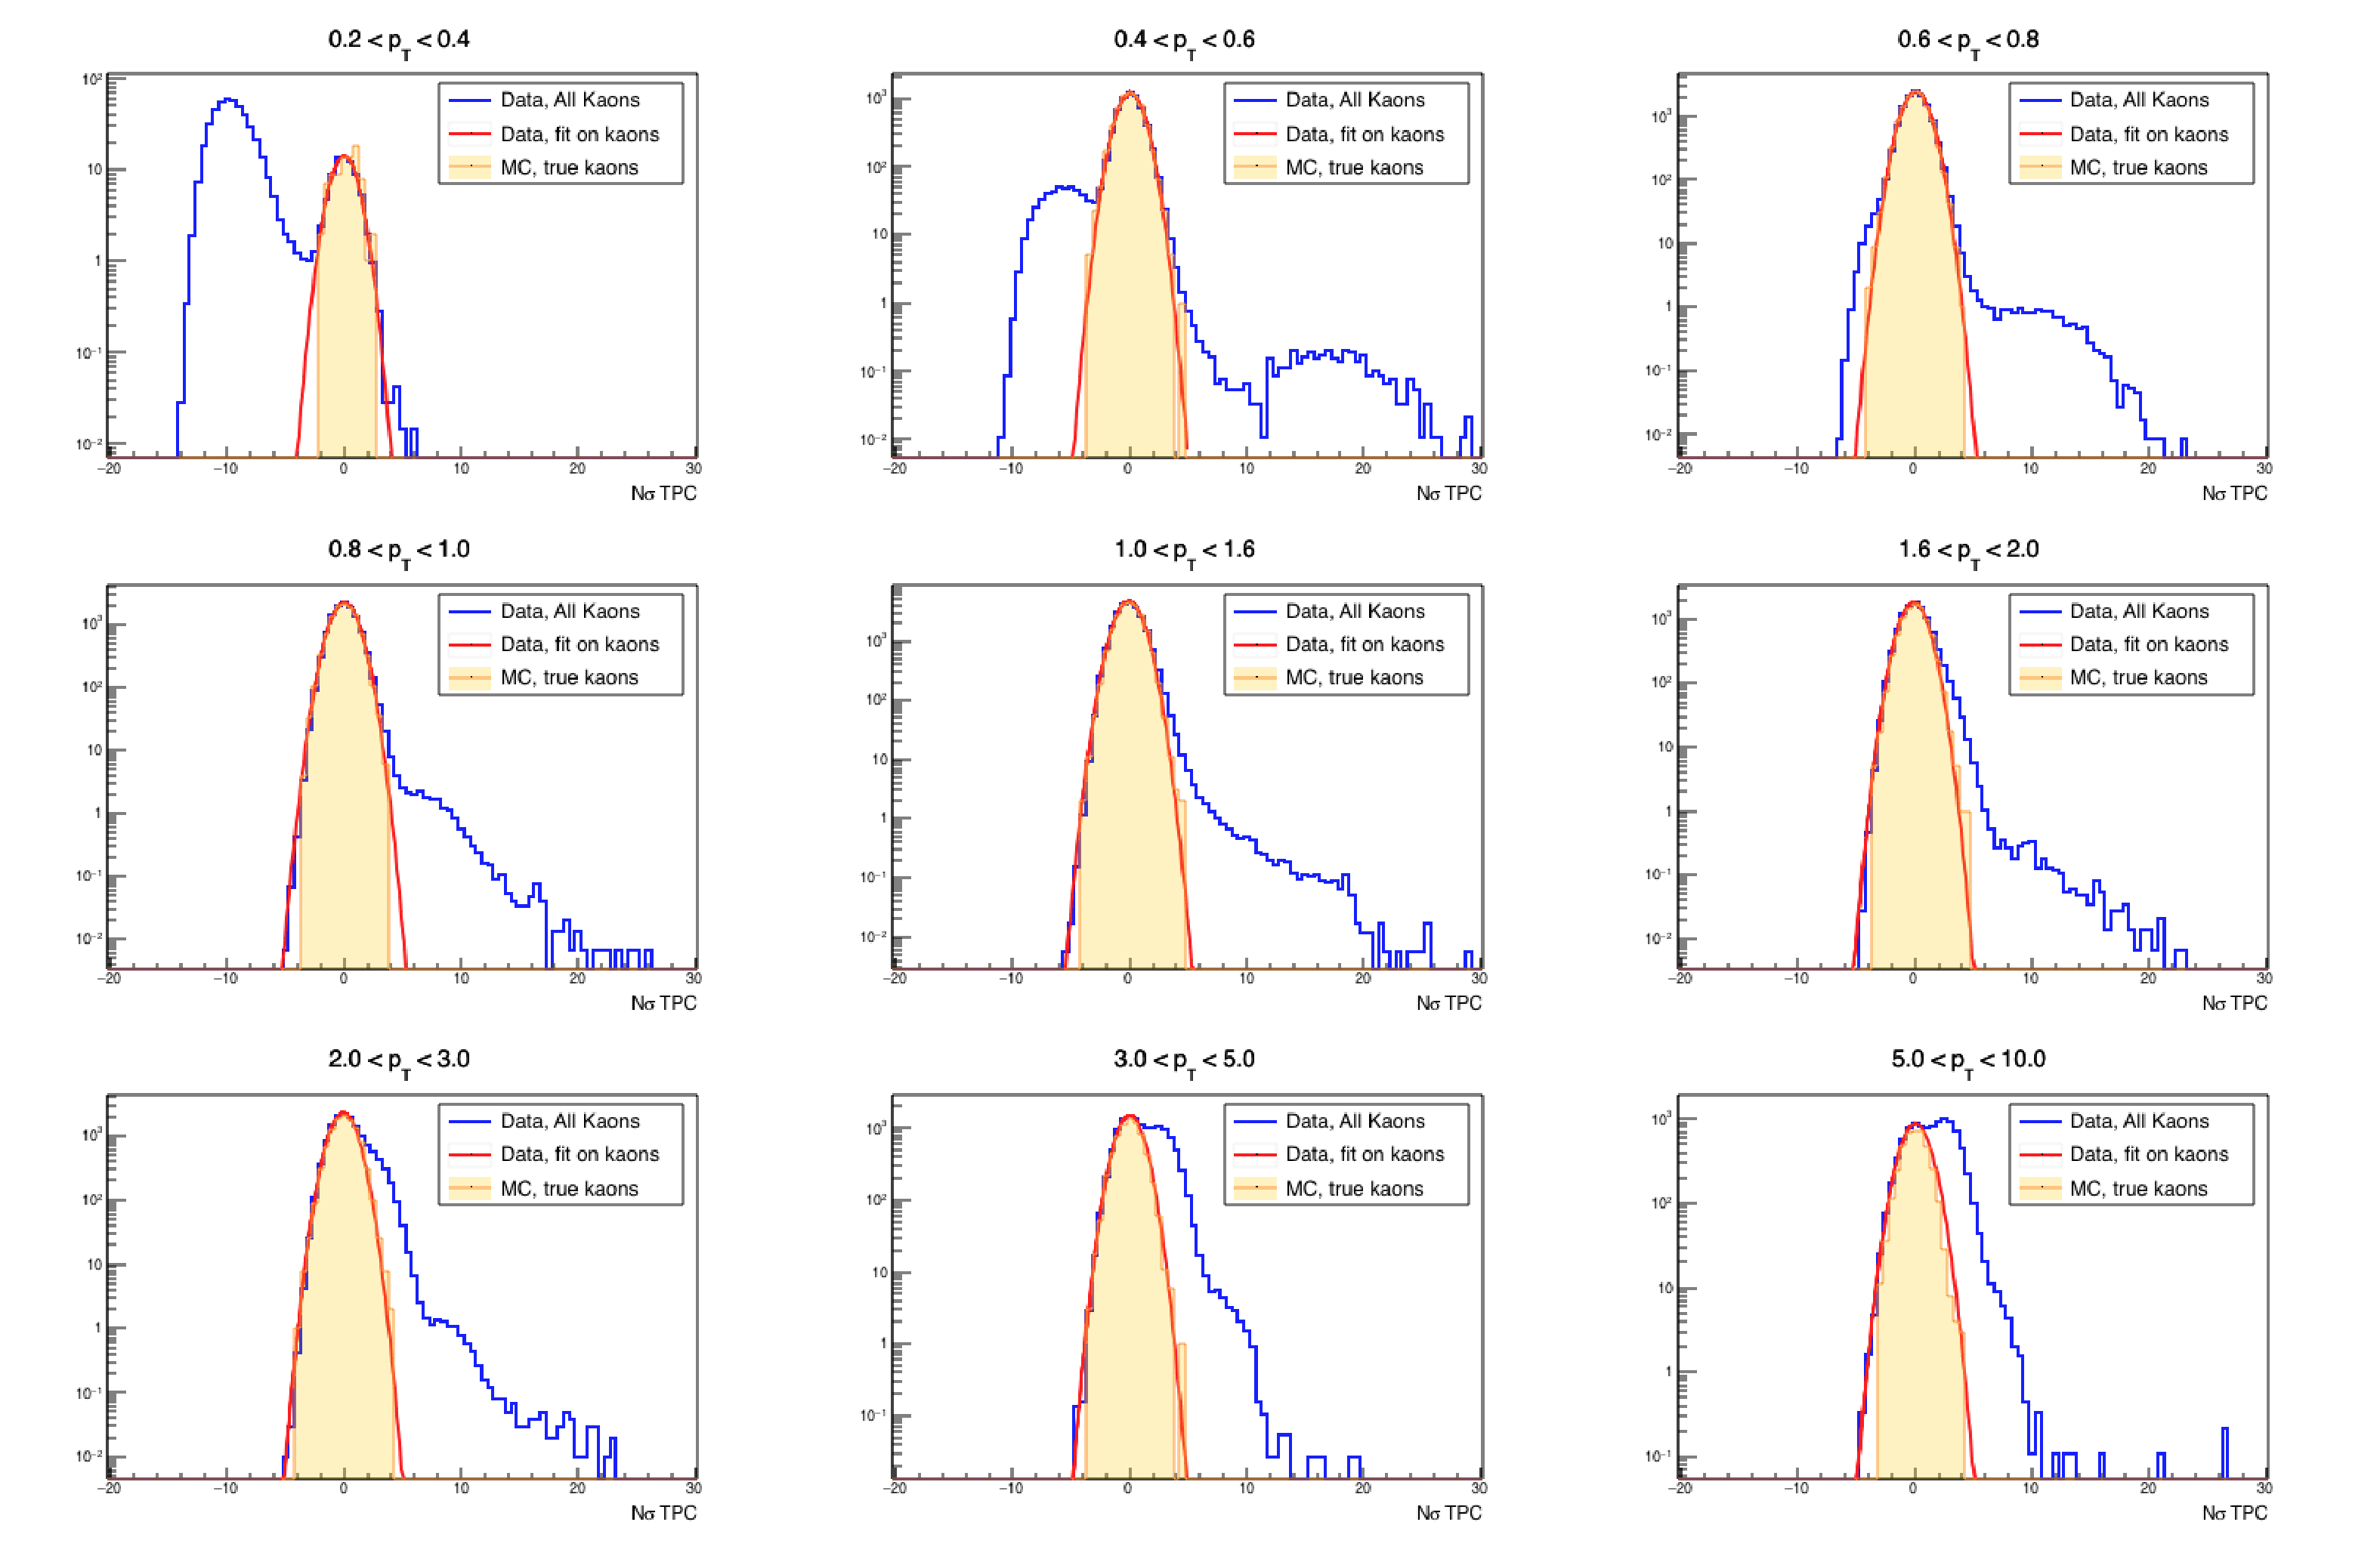
\includegraphics[angle=0, width=13cm]{./FigCap5/DataKaonComponents.eps}
 \caption{N-sigma distribution for dE/dx signal in TPC from kaon hypothesis in data, after a cut at sigma $<$ 0.25 from kaon hypothesis for TOF signal. In yellow, contribution from true kaon superimposed to data. In red, the fit to extrapolate the kaon component in the inclusive distribution.}
 \label{fig:DataPionsTOF} 
\end{figure}

\begin{figure}[!h]
 \centering
 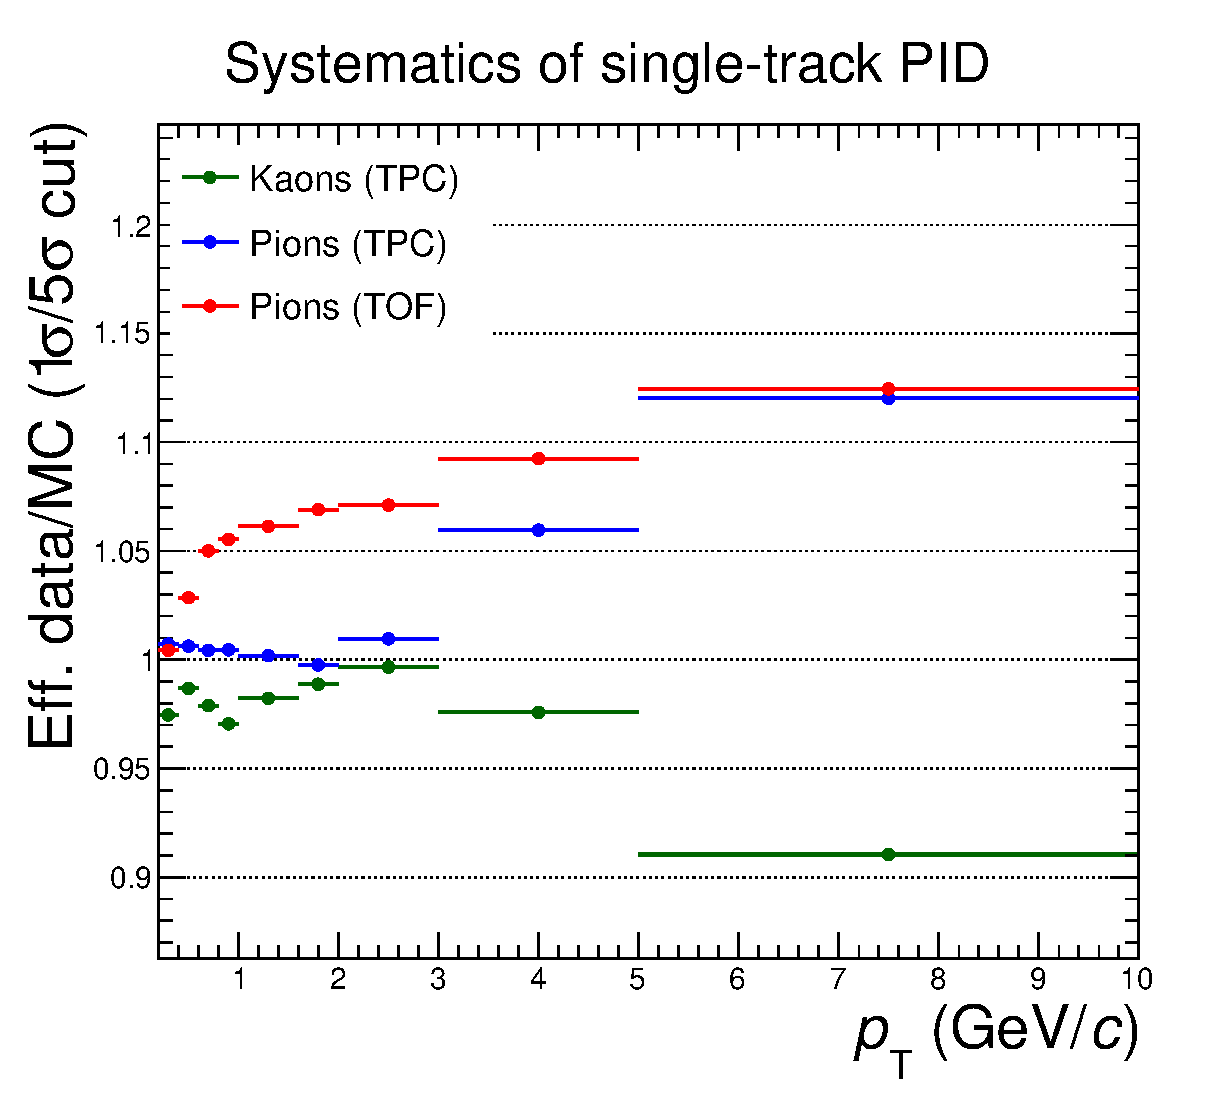
\includegraphics[angle=0, width=13cm]{./FigCap5/PIDsyst_1over5sigmaCut.eps}
 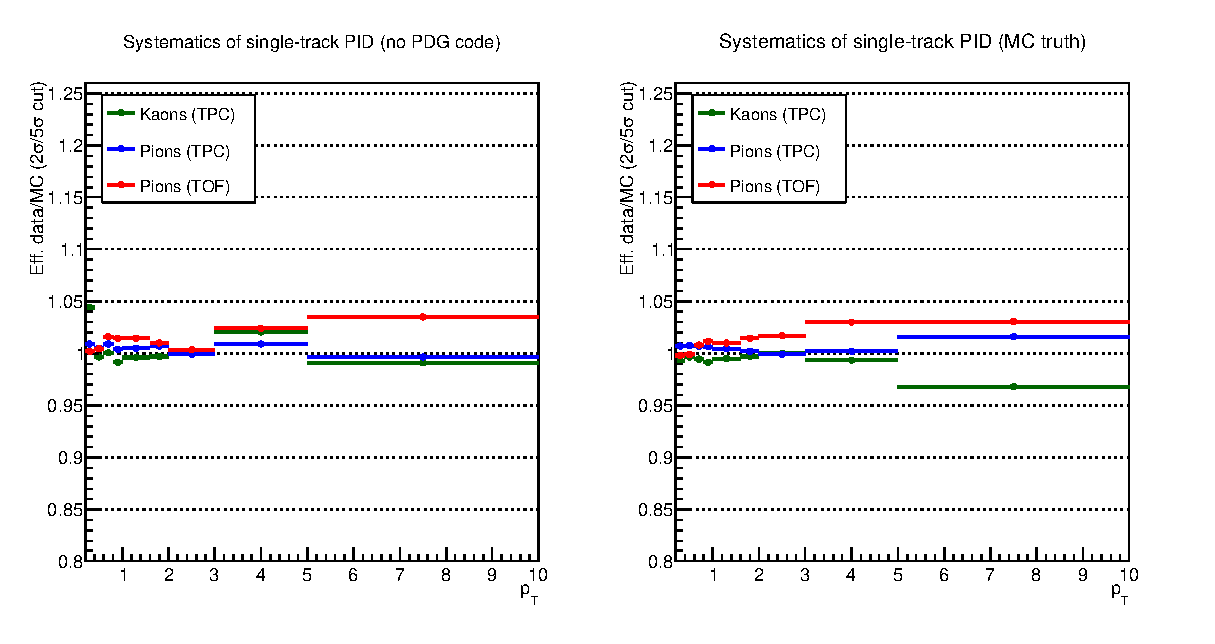
\includegraphics[angle=0, width=13cm]{./FigCap5/PIDsyst_2over5sigmaCut.eps}
 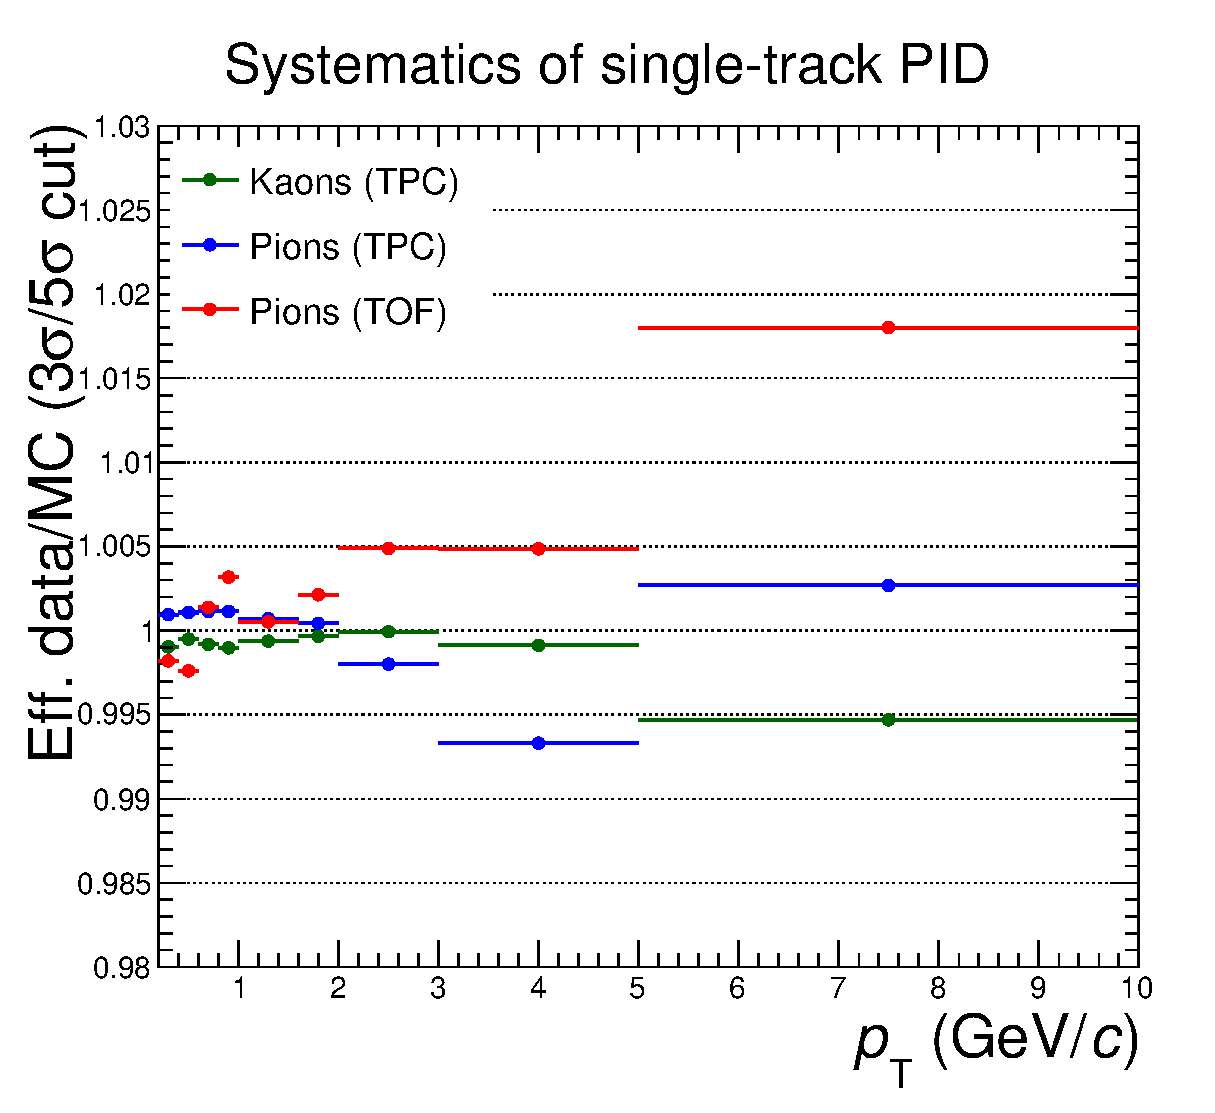
\includegraphics[angle=0, width=13cm]{./FigCap5/PIDsyst_3over5sigmaCut.eps}
 \caption{Per-track systematics for kaons and pions in TPC and TOF in different colours, as a function of $\pt$, for different N-sigma selection (1-sigma cut in the top panel, 2-sigma cut in the middle panel, 3-sigma cut in the bottom panel) with respect to a 5-sigma cut. Left and right panel refers to the Monte Carlo efficiency calculated on the distribution respectively without and with PDG code selection.}
 \label{fig:PerTrackPIDsys} 
\end{figure}

\begin{figure}[!h]
 \centering
 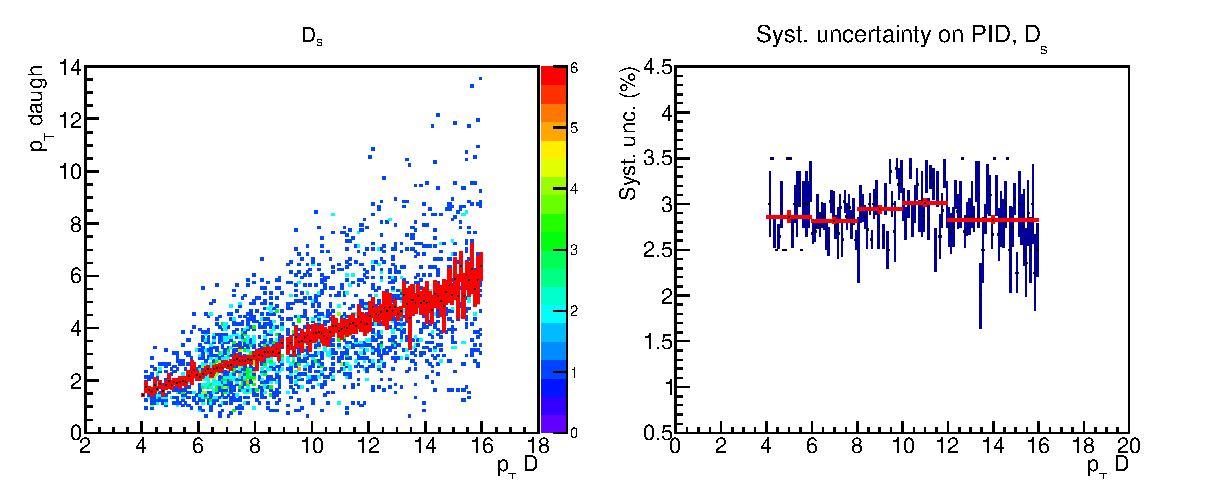
\includegraphics[angle=0, width=13cm]{./FigCap5/PIDsystDs_MCtruth.eps}
 \caption{Left: scatter plot of daughter's $\pt$ and $\Ds$-meson $\pt$. Right: systematics on PID for $\Ds$ meson as a function of $\pt$.}
 \label{fig:PerTrackPIDsys} 
\end{figure}

\subsubsection{Generated $\pt$ shape}
Another source of systematic uncertainty we investigated is the one arising from the D-meson 
$\pt$ shape assumed in the Monte Carlo used for corrections. The strategy adopted to check 
the stability of our efficiencies against different $\pt$ shapes and to define a systematic 
uncertainty is similar to the one used for the 30--50\% centrality class, described in section. 
In particular, the central value of the efficiency was computed 
applying the $\pt$ weights obtained from the the FONLL and BAMPS predictions for the 
60--80\% centrality class. For the 0--10\% centrality class, the re-weighted shape was obtained 
from the mixture of the measured $\Dzero$ corrected yield shape with FONLL predictions, 
used in the $\pt$ regions where the measurement is not feasible or not precise. 
Then, several other $\pt$ weights were considered to check the stability of the efficiencies 
against the $\pt$ shape of the generated D mesons. For the 60--80\% centrality class, 
the systematic uncertainty was evaluated comparing the central values of the efficiency 
to that obtained applying the FONLL weights, while for the 0--10\% centrality class the 
efficiency obtained using the FONLL times LBT and FONLL times TAMU weights were 
considered for the non-strange D mesons and the $\Ds$ respectively. 
In addition, for the $\Dplus$ the efficiency obtained with the $\Dzero$-shape $\pt$ weights was 
compared to that obtained from the measured $\Dplus$ corrected yield to check 
the consistency of the procedure. The difference between the two data-driven weights 
was found to be small, except for the first $\pt$ interval, where the measurement of the 
shape of the $\Dplus$ corrected yield was not feasible.
For the LBT weight, the systematic uncertainties for it may come large for the bin 2-3 GeV/c, 
because the model predicts the maximum value of the $\RAA$ to be at 3 GeV/c, unlike the other models, 
which leads the shape to be different for that $\pt$ region, but anyhow it's a possible shape can be considered.
 
In FigCap5 
are reported the outcomes of the check for the $\Dstar$, $\Dzero$and also $\Dplus$ meson 
in the case of FONLL and BAMPS weights. 
In Fig.\ref{DsMCshape_010_6080} there is the same plot for the $\Ds$ meson.
The values assigned as systematic uncertainty for all the non-strange D mesons are reported in 
Table  for the $\Ds$, where they are taken from the RMS
of a flat distribution in each $\pt$ interval summed in quadrature with the mean shift of the distribution itself. 



\begin{figure}[!htp]
\begin{center}
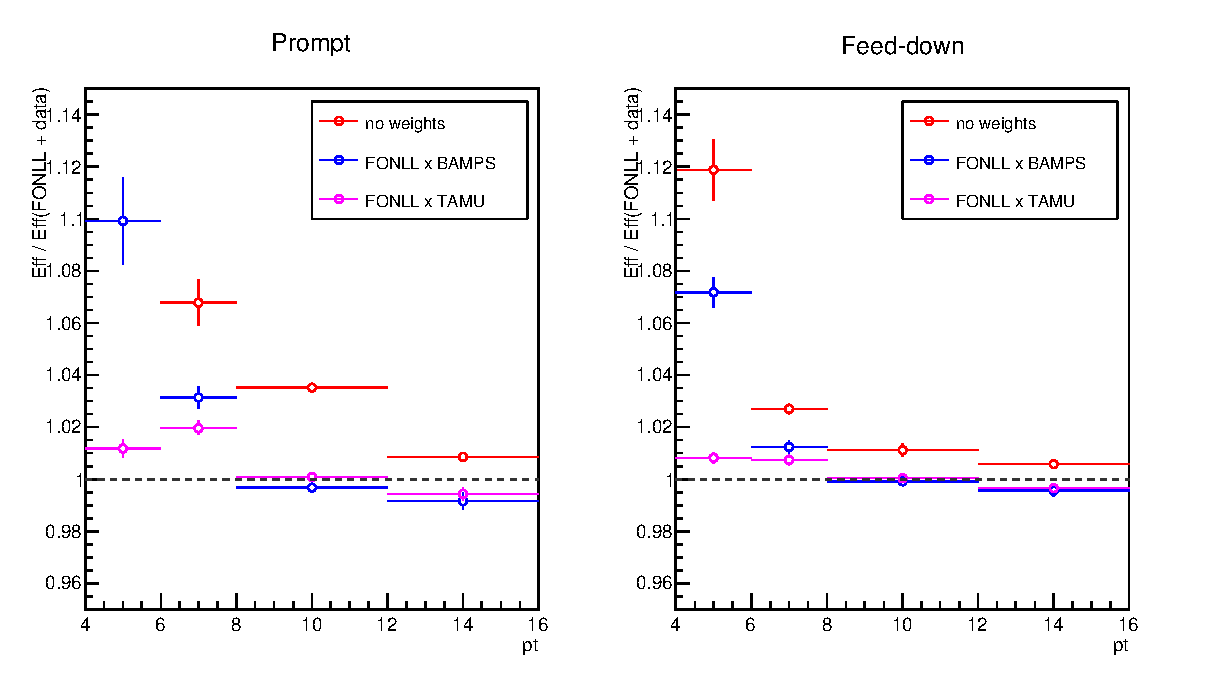
\includegraphics[angle=0, width=11.cm]{./FigCap5/MCptweights010_overFONLLdata_617.eps}   
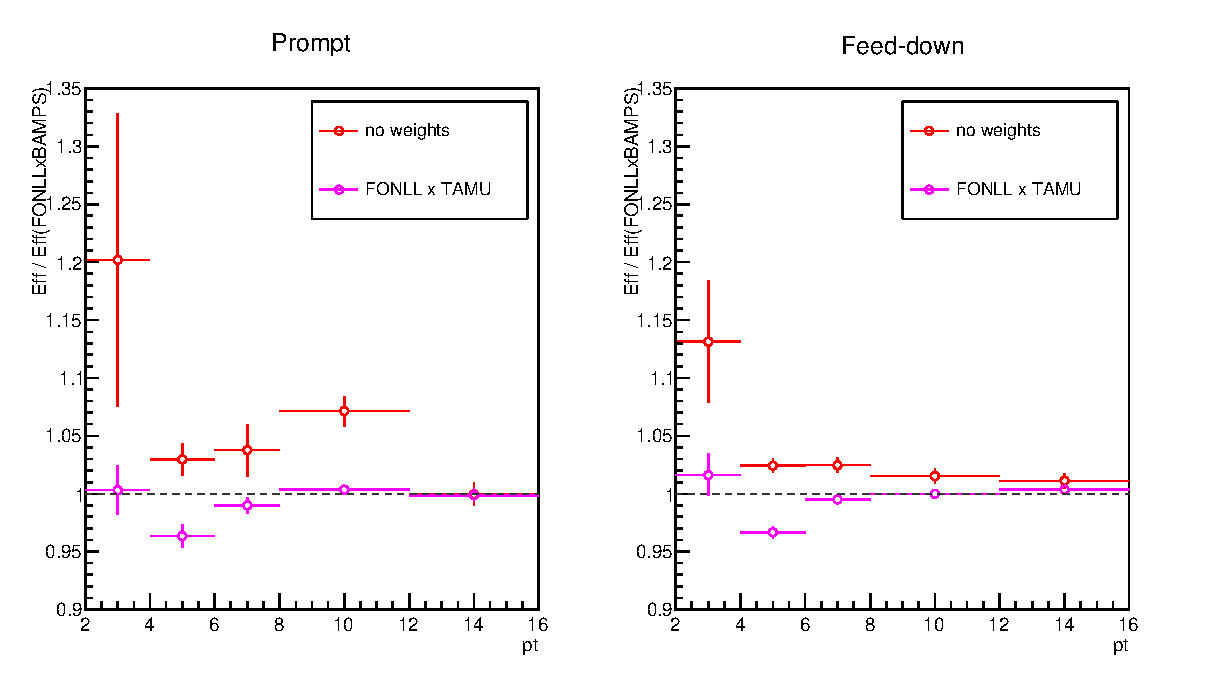
\includegraphics[angle=0, width=11.cm]{./FigCap5/MCptweights6080_overFONLLBAMPS_618.eps}   
\end{center}
\caption{Top: relative change of $\rm \Ds$ prompt and feed-down efficiencies in the 0--10\% centrality class by using FONLL  x BAMPS (blue), no (red) $\pt$-weights, or FONLL x TAMU (magenta) with respect to case of $\Dzero$ data-driven weights (default). Bottom: relative change of $\rm \Ds$ prompt and feed-down efficiencies in the 60--80\% centrality class by using no (red) $\pt$-weights, or FONLL x TAMU (magenta) with respect to case of FONLL x BAMPS weights (default).}
\label{DsMCshape_010_6080} 
\end{figure}

Additional systematic sources, deriving from the pp reference,
tracking efficiency, the B feed-down strategy and the hypothesis on
the $\RAA$ of D meson coming from B mesons decays, will be treated in
the next few sections. 

The systematic uncertainties on the $\Raa$ measurement include those 
on the D-meson corrected yields described above, those on the
proton--proton reference cross section, and the uncertainties on the
average nuclear overlap function. 

The uncertainty on the pp reference used for the calculation of $\RAA$ 
has two contributions. The first one is the systematic uncertainty on the measured 
$\pt$-differential D-meson cross section at $\sqrt s=7$~TeV.
The second contribution is the scaling to 
$\sqrt s = 5.02$~TeV, which was already discussed in Section.

In the calculation of the nuclear modification factor, the systematic 
uncertainty on the feed-down subtraction deriving from
the variation of the parameters of the FONLL calculation was considered to be
correlated in the $\PbPb$ and pp measurements, while all the other sources of systematic uncertainties were treated as uncorrelated.

The uncertainties on the $\RAA$ normalisation are the quadratic sum of 
(i) the pp normalisation uncertainty  (3.5\%), 
(ii) the uncertainty on $\langle T_{\rm AA} \rangle$, which ranges from 3.3\% to 6.2\% depending on the centrality, and
(iii) the uncertainty on the fraction of the hadronic cross section used in the 
Glauber fit to determine the centrality ($<0.1\%$, $2\%$ and $3\%$ for the 0--10\%, 30--50\% 
and 60--80\% centrality classes, respectively)~\cite{Adam:2015sza}, while the branching ratio uncertainty cancels out in the 
ratio.



\section{proton-proton reference}

The proton-proton reference we use to evaluate the D meson nuclear modification factor is based on a theoretical 
scaling of the published D cross sections at $\sqrt{s}$ = 7 TeV. The procedure to obtain it is 
explained in detail in . The updated pp cross section obtained from the analysis of the pass4 2010 data  is used for the results presented in this analysis.


\subsection{Feed-down subtraction}
The evaluation of the fraction of prompt D mesons and the systematic uncertainty due to the evaluation of the feed-down contribution is described in Section~\ref{sec:feeddown}. The only difference is in the hypothesis of the feed-down D-meson $\RAA$ in the 60-80$\%$ centrality class, since the measurement of the nuclear modification factor for prompt D meson is closer to unity with respect to the $\RAA$ for the central and the semi-central events. Therefore, the assumpion $\RAA^{\rm feed-down}=2\RAA^{\rm prompt}$ would imply a nuclear modification factor for feed-down D mesons larger than 1. As a consequence, in this case the central hypothesis is $\RAA^{\rm feed-down}=1.3\RAA^{\rm prompt}$ and it was varied between 1 and 1.6 to assgn a systematic uncertainty.
Fig.shows the fraction of prompt $\Dplus$ (right) and the variation of $\RAA^{\rm prompt}$ as a function of the hypothesis for  $\RAA^{\rm feed-down}/\RAA^{\rm prompt}$ for the 0-10$\%$ and the 60-80$\%$ centrality classes.

\section{Track reconstruction efficiency}
\label{sec:TrackCutsUnc_3050}
The systematic uncertainty related to the tracking efficiency includes the 
effects arising from track finding in the TPC, from track propagation  
from the TPC to the ITS, and from track quality selections.
It was estimated with the following tests:
\begin{itemize}
\item comparison of the $\Dplus$ cross sections obtained with different track selection cuts;
\item comparison of the TPC-ITS track matching efficiency in data and simulations.
\end{itemize}
These checks are discussed in detail in the following subsections.

\subsection{Variation of track selections}

The D-meson raw yields, efficiency and corrected yields were evaluated with 
different sets of track selection cuts.
Only one cut at a time was changed with respect to the standard values 
reported in Section.
In particular, for the $\Dplus$ meson, the following four cut variations were 
tested:
\begin{enumerate}
\item additional cut on number TPC crossed rows $> 120-(5/\pt)$;
\item number of TPC clusters $>0.65 \times$ number of TPC crossed rows;
\item additional cut on number of clusters with TPC dE/dx signal $> 0.5 \times$ number of TPC crossed rows;
\item ratio of crossed rows over findable clusters in the TPC $>0.9$.
\end{enumerate}

The results are reported in fig., where the
left panel show the ratio of the prompt efficiencies with the different set of cuts 
and the one from the standard cuts; the right panel shows the ratio for the corrected yield of
 $\Dplus$ mesons with the various track-cut selections and the default one.
For the comparison of the corrected yields, one can see that a systematic 
deviation of, on average, about 3\% is observed when varying the cut on the ratio of 
crossed rows. The cuts on the TPC over crossed rows doesn't contribute to the systematic uncertainty
because this is not a cut used in the analysis.
Based on these results, a 3\% systematic uncertainty was assigned.
$\Dplus$ are reconstructed from a three-body decay
channel, so one could account for a 1\% systematic uncertainty per track.
For this reason, the 3\% uncertainty estimated with the $\Dplus$ was
assigned also to the $\Ds$ mesons, which are also reconstructed via a 
three-body decay and for which the lower statistical significance 
does not allow to estimate the systematic uncertainty with the same
precision obtained for the $\Dplus$, and a 2\% to the $\Dzero$, for which the two-body decay channel
is analysed.

\subsubsection{Systematic uncertainties FOR V2}
\label{systsection}

The sources of systematic uncertainty affecting the measurement of $\Dzero$, $\Dplus$ and $\Ds$ $v_2$ with the event plane method that we are considering are:
\begin{itemize}
\item{the systematic uncertainty on the yield extraction from the invariant mass distributions}
\item{the systematic uncertainty coming from the variation in the measured $v_2$ with different sets of cuts. Since we do not use efficiencies extracted 
from the Monte Carlo, the cut variation is not aimed at estimating the residual
differences between data and simulations in the description of the cut 
variables. Rather it tests the stability of $v_2$ extraction against variations
of the significance and signal over background of the D meson peaks.}
\item{the systematic uncertainty due to the event plane resolution variation 
inside the wide centrality bin. The measured D mesons, whose production 
scales with the number of binary nucleon-nucleon collisions, are preferentially
coming from more central events inside the considered bin}
\item{the systematic uncertainty related to the flatness of the event plane distribution}
%\item{the systematic uncertainty due to the difference in the
%event plane resolution estimated with different methods.}
\end{itemize}

The signal extraction is performed with a fit to the invariant mass
distribution of the candidates, under the assumptions of an
exponential shape for the background for $\Dzero$, $\Dplus$ and $\Ds$. For the signal a Gaussian shape was assumed for all of the three mesons.  
The width of the Gaussian fit is fixed fitting the invariant mass distribution of the candidates on the full azimuthal angle. Thus, when splitting the distribution in the in-plane versus out-of-plane azimuthal angles the Gaussian $\sigma$ is not a free parameter anymore. 
The systematic uncertainty on the yield extraction was estimated by varying the fit parameters, namely the background fit function
(exponential vs. parabola and linear function), the invariant mass bin
width and the fit range, with a multi-trial approach. The same multiple
trials were performed by fitting in the two
$\Delta\phi$ bins without fixing the Gaussian $\sigma$ to the value
extracted from the $\phi$ integrated distribution and extracting the
D-meson raw signal via a bin-counting procedure. The distributions of
residuals, $v_2^{trial}-v_2^{ref}$, were obtained for each $\pt$ bin
considering the 4 options (fits in-plane and out-of-plane with and
without fixed sigma and extraction of the raw yields with two bin
counting methods). The systematic uncertainty was evaluated
considering both the shift with respect to zero and the RMS of the residuals
distributions obtained from the fits fixing the sigma to the values
obtained from $\varphi$-integrated distributions. The residuals
distributions obtained with free sigma and the two bin counting
methods were also compared with those obtained fixing the sigma, and, the
shift with respect to zero and RMS taken into account in the
evaluation of the uncertainties in case of systematic deviations with
respect to the fixed sigma results.
The residuals distributions are reported in Fig. for the $\Dzero$, in Fig. for the $\Dplus$ and  in Fig. for the $\Dstar$. 

 In the case of $\Ds$, the mean value of the residual distribution, together with its error (the RMS of the residual distribution), for the different trials using the fit with single or double Gaussian, and with free/fixed sigma, is shown in Fig.~\ref{fig:Dsv2residuals} for the different $\pt$ intervals.

The assigned absolute values of the yield extraction systematic uncertainties for $\Dzero$, $\Dplus$ and $\Dstar$ are summarised in table.


The analysis was also performed with different sets of cuts for the 
D meson selection and a systematic uncertainty was assigned to account for the 
variation in the measured $v_2$ with the different sets of cuts.
The left plot in Fig. shows the $\Dplus$ $v_2$ 
results with 9 different sets of cuts (4 looser, 4 tighter and the default one). 
In the right plot of the same Figure are shown the residuals of the $\vtwo$ obtained for each different set of topological cuts with respect to the default result. Since the residuals do no show 
any particular trend or hierarchy, and they are almost all within 1
$\sigma$ of the statistical plus the yield extraction uncertainties
summed in quadrature (grey band), no systematic uncertainty was
assigned for the cut variation study. 
\begin{figure}
 \centering
 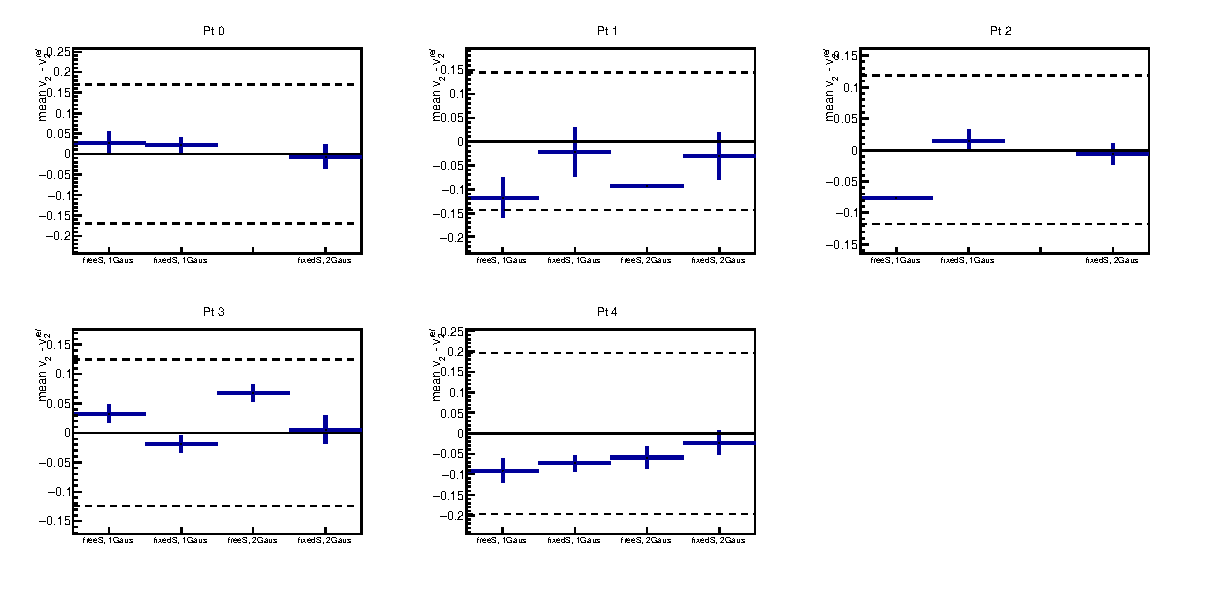
\includegraphics[width=.9\textwidth]{FigCap5/resultsComparison_sFixToMC_ExpoLin.eps}
 \caption{Mean values of the residual $\vtwo-\vtwo^{ref}$ distributions for $\Ds$
   meson. Uncertainties are the RMS of such distributions.}\label{fig:Dsv2residuals}
\end{figure} 


An other source of systematic uncertainty that was considered is 
related to the event plane resolution.
The centrality dependence of the event plane resolution 
(see left panel of Fig.~\ref{fig:dplus-4ep} as an example) gives rise to
an uncertainty because the centrality bins used to measure the D meson
yield are wide and D meson production (scaling as the number of binary 
collisions) is more probable in more central events.
The uncertainty owing to the centrality dependence of the EP
resolution was estimated from the difference between two ways to
define the average resolution in the centrality class used in the
analysis, starting from the resolutions in fine centrality intervals,
namely, a plain arithmetic average and an average weighted with the
D-meson yield measured in smaller centrality classes and
with $N_{\rm coll}$ values (2.5\% wide). The
latter was estimated using $\Dzero$ meson raw yields in wide $\pt$
intervals (2-4, 4-8, 8-16 $\GeV/c$) and the sum of the two $\varphi$
intervals, to reduce the statistical fluctuations. The difference
between these averages was found to be about 2\% for the 30–50\%
centrality class.


Furthermore, as an additional check the resolution was re-computed introducing 
a pseudorapidity gap between the sub-events, in order to estimate a possible bias 
in the event plane resolution due to non-flow contributions. In particular it was considered an eta 
gap of 0.1 and 0.2 between the sub-events computed using the TPC tracks with positive/negative 
eta. The left panel of Figure \ref{fig:EtaGapSyst} shows the comparison of the event plane resolution
as a function of centrality computed without eta gap, with an eta gap of 0.1, with an eta gap 0.2. 
In the latter case the resolution was also computed applying the $\pt$ weights in the measurement of
the event plane of the two sub-events obtained from the tracks in the TPC.
In the right plot of the same Figure the corresponding relative variation of the event plane resolution is shown.
Considering this observation an additional 1\% systematic uncertainty on the determination of the
event plane resolution was assigned.

\begin{figure}
\centering
  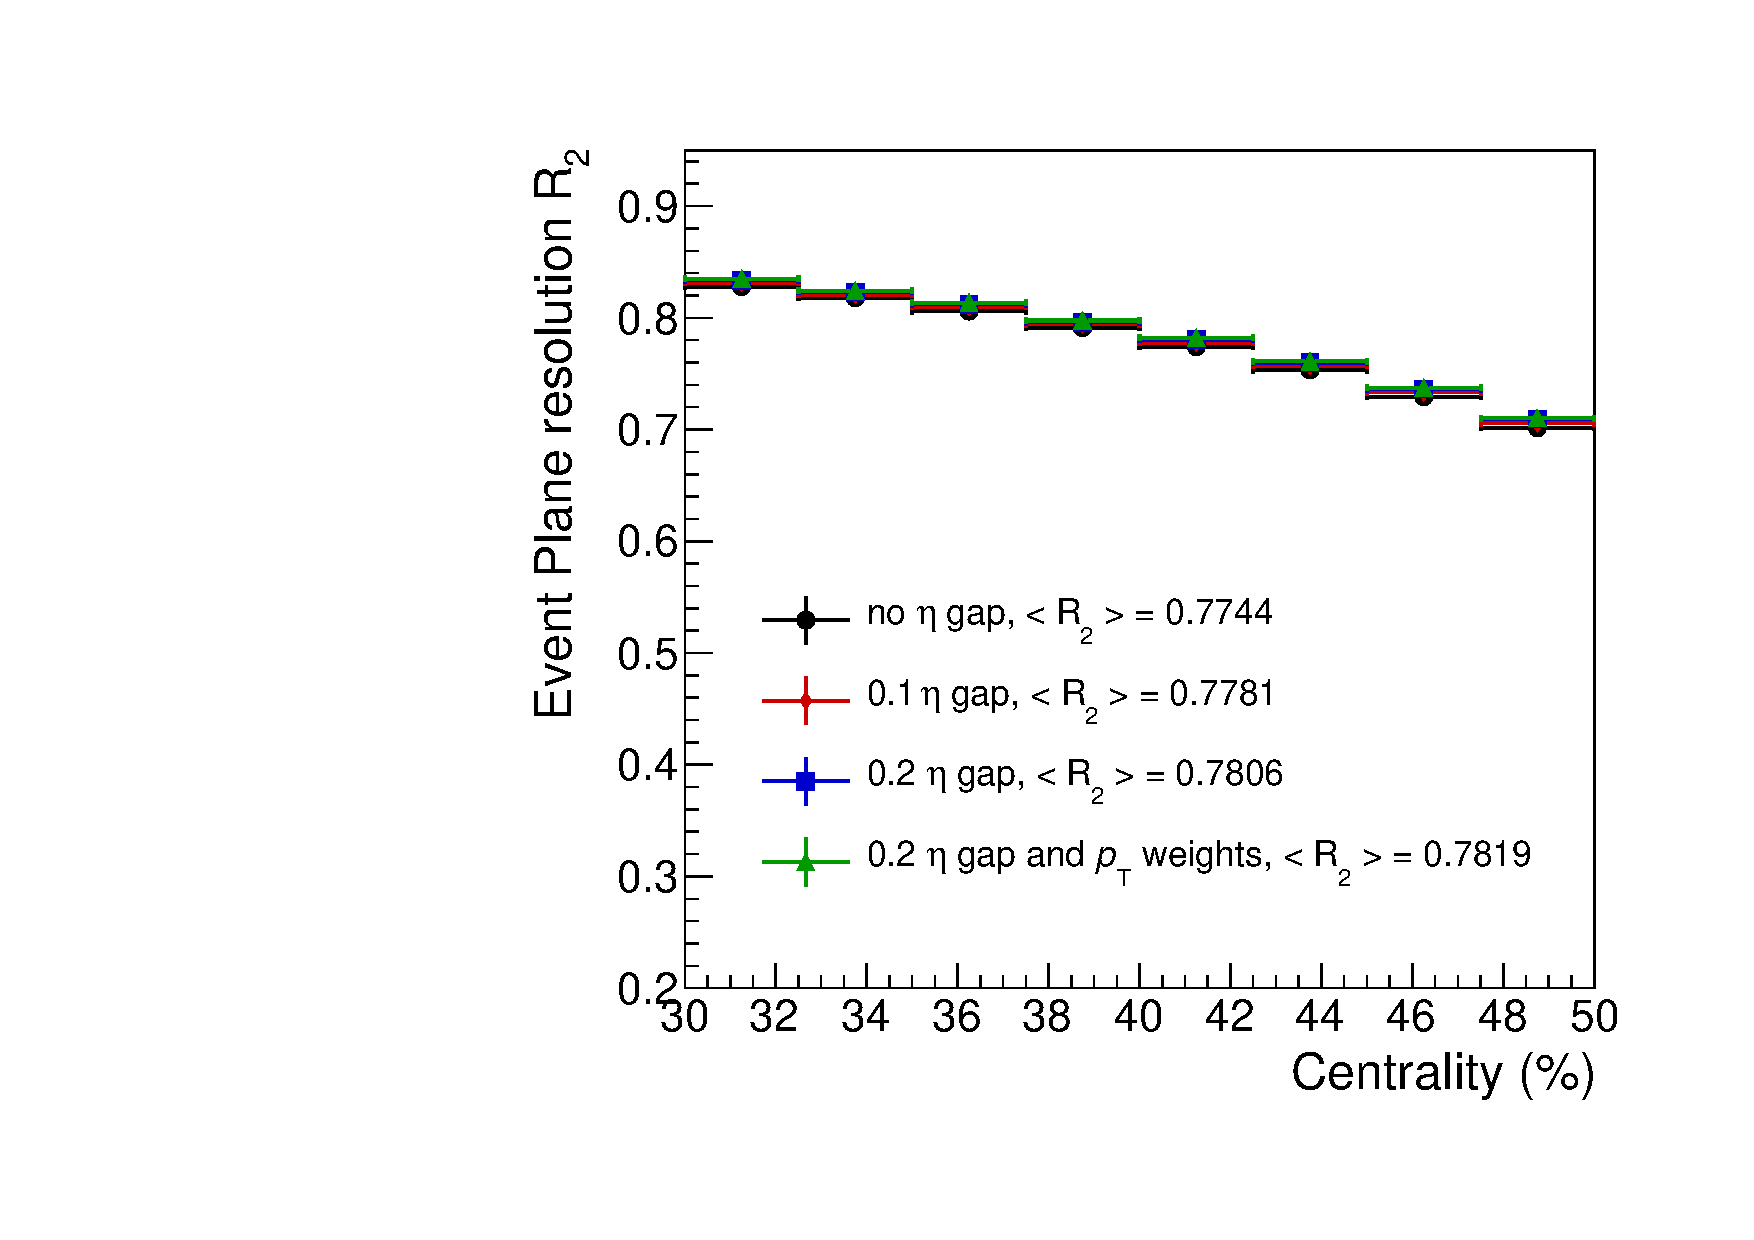
\includegraphics[width=.45\textwidth]{FigCap5/EPresolution_VZERO_NonFlowSyst.pdf}
  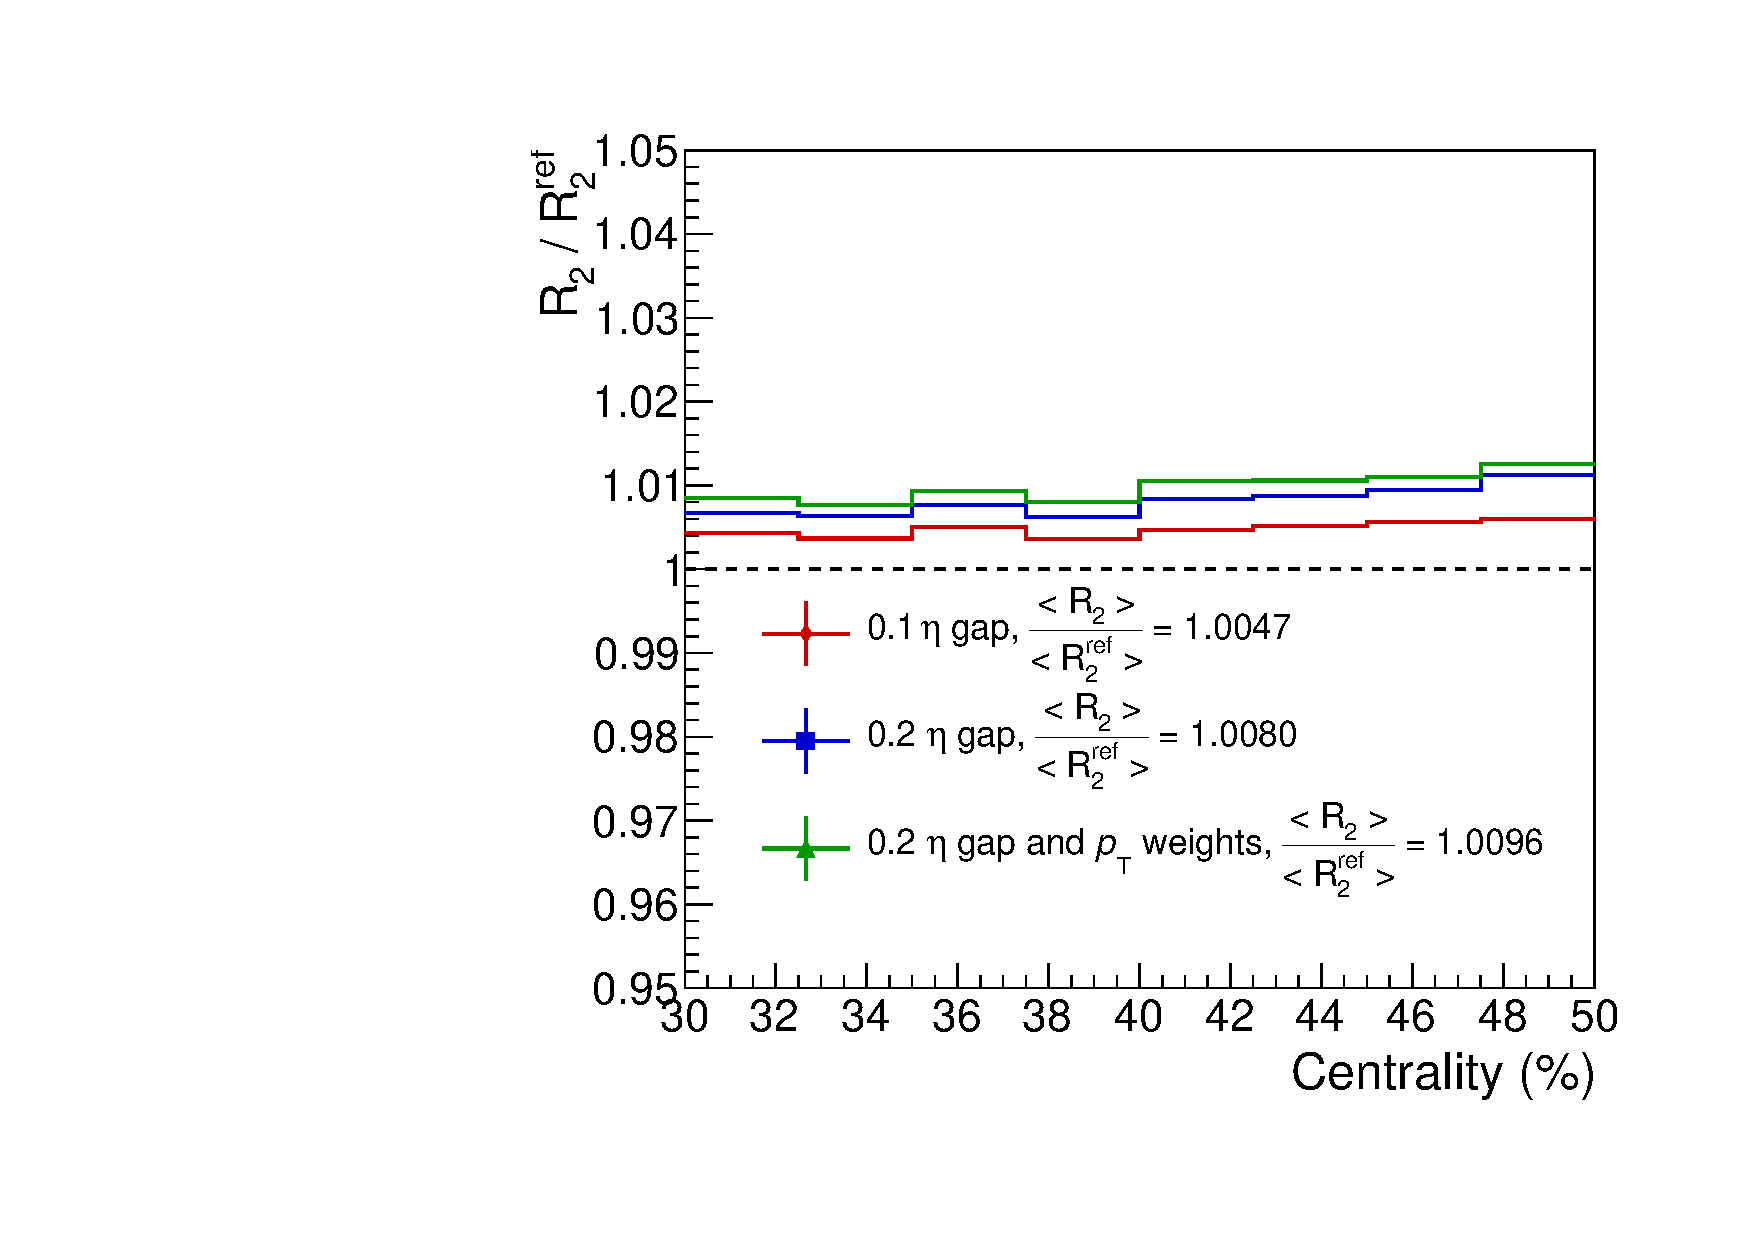
\includegraphics[width=.45\textwidth]{FigCap5/EPresolution_VZERO_NonFlowSyst_ratio.pdf}
\caption{Event plane resolution as a function of centrality estimated introducing an eta gap between the sub-events computed using the TPC tracks (left) and the corresponding relative variation with respect to the default configuration (right).}
\label{fig:EtaGapSyst}
\end{figure}

The event plane was measured using the multiplicity in the VZERO
detector. The resolution on the event plane was estimated by considering 3
sub-events: VZERO multiplicity, TPC tracks in the positive eta region
and TPC tracks in the negative eta region. The event plane was also
measured considering TPC tracks in the positive eta region, all the
TPC tracks and the multiplicity in the C-side of the VZERO
detector. The resolution was calculated considering two or three
sub-events for the event plane measured with TPC tracks in the
positive eta region, and with three sub-events when considering the
full TPC or the C-side of the VZERO detector for event plane
measurement. The best resolution is obtained considering the event
plane measured with full TPC, while the lowest resolution using the
the C-side of the VZERO detector, due to the limited acceptance. The
resolution obtained with three sub-events and full VZERO for the event
plane measurement and the resolutions obtained with two or three
sub-events when using TPC tracks in the positive eta region for the
event plane estimate are very similar. The
measurement of the event plane with the VZERO detector at forward
rapidity and the correlation with D meson candidates at mid-rapidity
should allow a better rejection of non-flow correlations with respect
to the measurement of the event plane considering tracks in the same
eta region of the D meson candidates (TPC event planes).
The comparison between the $v_2$ of $\Dplus$ mesons obtained with 
different event planes is reported in 
Fig.~\ref{fig:dplus-4ep} for the 30-50\% centrality class. 
The current uncertinties on the $v_2$ values do not allow to
appreciate different non-flow contributions using different detectors
for the event plane measurement, thus, introducing different
rapidity gaps between the tracks used for the event plane measurement
and the D mesons.

\begin{figure}
\centering
  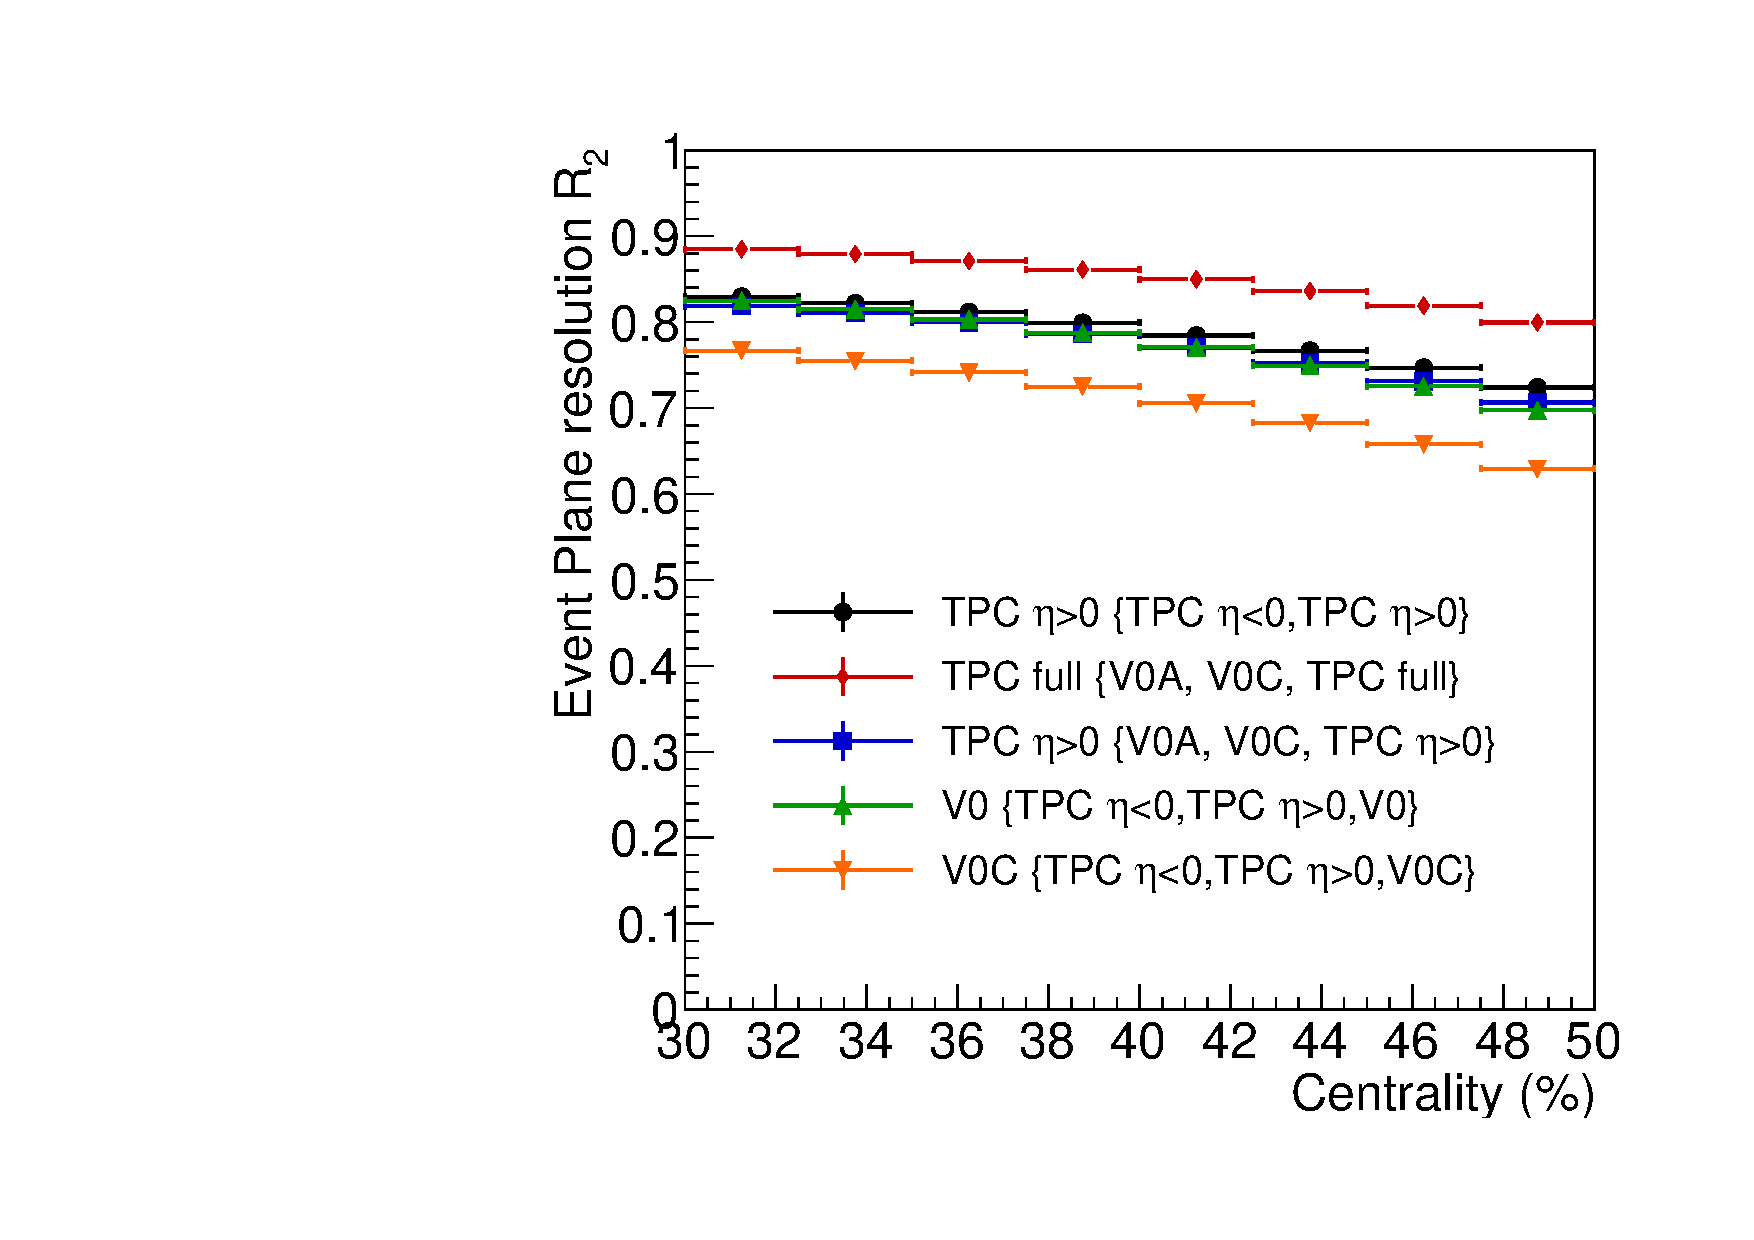
\includegraphics[width=.45\textwidth]{FigCap5/EPresolution_comparison.pdf}
\caption{$R_2$ resolution as a function of centrality estimated with 5 different detector configurations (left) and $v_2$ of $\Dplus$ as a function of $\pt$ for 30--50\% centrality class with 5 different event planes with different detector configurations (right).}
\label{fig:dplus-4ep}
\end{figure}


In order to check the flatness of the event plane distributions several checks have been performed for the main configuration used (main event plane measured with the multiplicity in the full VZERO and resolution estimated with 3 sub-events). In particular, if we consider that
\begin{equation}
\cos(2\Delta\phi) = \cos(2\phi_D-2\psi_{EP}) = \cos(2\phi_D)\cos(2\psi_{EP})+\sin(2\phi_D)\sin(2\psi_{EP}),
\end{equation}
where $\phi_D$ is the azimuthal angle of the D meson and $\psi_{EP}$ the azimuthal angle of the event plane, a non-zero value of $< \cos(2\phi_D) >/R_2 \times < \cos(2\psi_{EP}) >/R_2$ (and the same for the sine) would lead to a bias in the measurement of the D-meson $\vtwo$. The  $< \cos(2\psi_{EP}) >$ and $< \sin(2\psi_{EP}) >$ factors have been extracted from the fits to the event plane distributions shown in Fig.. The fitting functions used are respectively 
\begin{equation}
N(1+2b\cdot \cos(2\psi_{EP}))
\end{equation}
and 
\begin{equation}
N(1+2b'\cdot \sin(2\psi_{EP})),
\end{equation}
where $b = < \cos(2\psi_{EP}) >$ and $b' = < \sin(2\psi_{EP}) >$.
In particular for the full VZERO, we can observe how the parameters extracted with this method are smaller than 0.001.


To estimate $< \cos(2\phi_D) >$ and $< \sin(2\phi_D) >$ have been used two methods:
\begin{itemize}
\item The subtraction of the $\cos(2\phi_D)$ ($\sin(2\phi_D)$) distribution of the combinatorial background from the distributions of the side-bands.
\item The fit of the $\cos(2\phi_D)$ ($\sin(2\phi_D)$) vs. the invariant-mass.
\end{itemize}

\section{B feed-down}
\label{feeddownsec}
The measured D meson yield includes a contribution (of about 85-90\%)
from prompt D mesons and a contribution from beauty feed-down, which give rise
to D mesons displaced from the primary vertex by hundreds of microns
due to the larger B meson lifetime.
The prompt component includes the D mesons produced directly in the 
hadronization of a c quark and those originating from the decay of an
excited state (D$^*$) produced by the c quark.
Considering that $v_2$ is additive, the measured $v_2$ is therefore given by:
\begin{equation}
\label{eq:bfeed}
v_2^{\rm obs}=f_{\rm prompt} v_2^{\rm promptD} + (1-f_{\rm prompt})v_2^{\rm feed-down}
\end{equation}
where $f_{\rm prompt}$ is the fraction of D mesons promptly produced in the measured
yield.
The value of $f_{\rm prompt}$ depends on the D meson species, the transverse
momentum interval, the applied cuts.
It is estimated using the FONLL prediction for B mesons, 
the B$\rightarrow$D decay kinematics from the EvtGen package and
the Monte Carlo efficiencies for feed-down D mesons. 
\begin{equation}
 \label{eq:fpNbMethod}
 \begin{split}
   f_{\rm prompt} &= 1-(N^{\rm D~feed-down~raw}/N^{\rm D~raw})=\\
   &= 1 - \langle \TAA \rangle 
   \cdot \left( \frac{{\rm d}^2 \sigma}{{\rm d}y \, {\rm d}\pt }
\right)^{{\sf FONLL}} _{{\rm feed-down}} \cdot \RAA^{\rm feed-down} \cdot
\frac{({\rm Acc}\times\epsilon)_{\rm feed-down}\cdot\Delta y \, \Delta\pt
\cdot {\rm BR} \cdot N_{\rm evt}  }{ N^{\rm D~raw }  / 2} \, ,
 \end{split}
\end{equation}
where $({\rm Acc}\times\epsilon)_{{\rm feed-down}}$ is the 
acceptance-times-efficiency for feed-down D mesons and the factor 2 at the denominator
accounts for considering particle and antiparticle in the analysis.
The nuclear modification factor of the feed-down D mesons, $\RAA^{\rm feed-down}$,
is related to the nuclear modification of beauty production in Pb--Pb 
collisions, which is expected to differ from that of charm. 
 Taking advantage of the
recent non-prompt J/$\Psi$ results from the CMS collaboration we
assumed for the correction that the nuclear modification factor 
for feed-down is equal to two times the one of the prompt D mesons ($\RAA^{\rm feed-down}=2\RAA^{\rm prompt}$) and varied this hypothesis
in the range $1<\RAA^{\rm feed-down}/\RAA^{\rm prompt}<3$ for non-strange D mesons, and in the range  
$1/3<\RAA^{\rm feed-down}/\RAA^{\rm prompt}<3$ for $\Ds$ mesons,
to determine the systematic uncertainty.

To estimate the contribution of the feed-down D mesons on the measured $v_2$ 
an hypothesis on the unknown $v_2^{\rm feed-down}$ of D mesons from B decays, 
which is sensitive to the dynamics of b quarks in the medium, is needed.
We assumed as range for the hypothesis on 
the anisotropy of feed-down D mesons $0<v_2^{\rm feed-down}<v_2^{\rm prompt}$.

The lower limit, $v_2^{\rm feed-down}=0$, corresponds to the assumption:
\begin{itemize}
\item{at low $\pt$, where $v_2$ is determined by collective motions, 
that b quarks do not flow with the medium and there is not contribution to 
the B anisotropy from the light quark}
\item{and at high $\pt$, where $v_2$ is determined by azimuthal dependent 
energy loss, due to different path length in-plane and out-of-plane, that
b quarks are not affected by the medium.}
\end{itemize}

The upper limit, $v_2^{\rm feed-down}=v_2^{\rm prompt}$, corresponds to assuming:
\begin{itemize}
\item{at low $\pt$ that b quarks are as thermalized as c quarks}
\item{at high $\pt$ that b quark energy loss is the same as that of c quarks}
\end{itemize}


The assumed range for $v_2^{\rm feed-down}$ includes the measured $v_2$ 
of non-prompt $J\psi$ at central rapidity~\cite{Khachatryan:2016ypw} and the available 
model predictions~\cite{Aichelin:2012ww,Uphoff:2012gb,Greco:2007sz,Gossiaux, BAMPS, Rapp}. 
In particular, we assumed a uniform probability distribution of $v_2$ in this interval. 
Therefore the central value of the prompt D-meson $v_2$ was assigned considering 
\begin{equation}
v_2^{\rm feed-down}=v_2^{\rm prompt}/2,
\end{equation}
while the systematic uncertainty was 
estimated by considering 1$\sigma$ variation ($\Delta v_2^{\rm feed-down}/\sqrt{12}$, with 
$\Delta v_2^{\rm feed-down} = v_2^{\rm prompt}$). 
The maximum and minimum values of $v_2^{\rm prompt}$ are then computed as
\begin{equation}
v_{2}^{\rm prompt}=v_{2}^{\rm obs}/f_{\rm prompt} - (1-f_{\rm prompt})/f_{\rm prompt}v_{2}^{\rm feed-down},
\end{equation} 
using respectively the minimum and the maximum values of $v_{\rm 2}^{\rm feed-down}$ and $f_{\rm prompt}$. 
The uncertainty on $f_{\rm prompt}$ was estimated 
computing a set of values in each $\pt$ bin by
varying the heavy quark masses and the factorisation and renormalisation 
scales in the FONLL calculation, and by varying the hypothesis 
on $\RAA^{\rm feed-down}/\RAA^{\rm prompt}$ in the range quoted above.
The factorisation and renormalisation 
scales, $\mu_{\rm F}$ and $\mu_{\rm R}$, were made to vary independently 
in the ranges $0.5<\mu_{\rm F}/m_{\rm t}<2$, $0.5<\mu_{\rm R}/m_{\rm t}<2$, 
with the constraint $0.5<\mu_{\rm F}/\mu_{\rm R}<2$, 
where $m_{\rm t}=\sqrt{\pt^2+m_{\rm c}^2}$.
The mass of the c and b quarks were varied within $1.3<m_{\rm c}<1.7~\gev/c^2$ 
and $4.5<m_{\rm b}<5~\gev/c^2$, respectively.
In Fig.~\ref{fig:fPrompt} the prompt fraction for the three D mesons is shown.
The error bars on the points in Fig.~\ref{fig:fPrompt} include the
contributions of the FONLL scales variations and of the variation of
the hypothesis on $\RAA^{\rm feed-down}/\RAA^{\rm prompt}$.

The systematic uncertainty on $v_2$ due to B feed-down contribution
was assigned as $1/f_{\rm prompt}$ taking the lowest of the
$f_{\rm prompt}$ values resulting from its lower uncertainty.


\begin{figure}
 \centering
 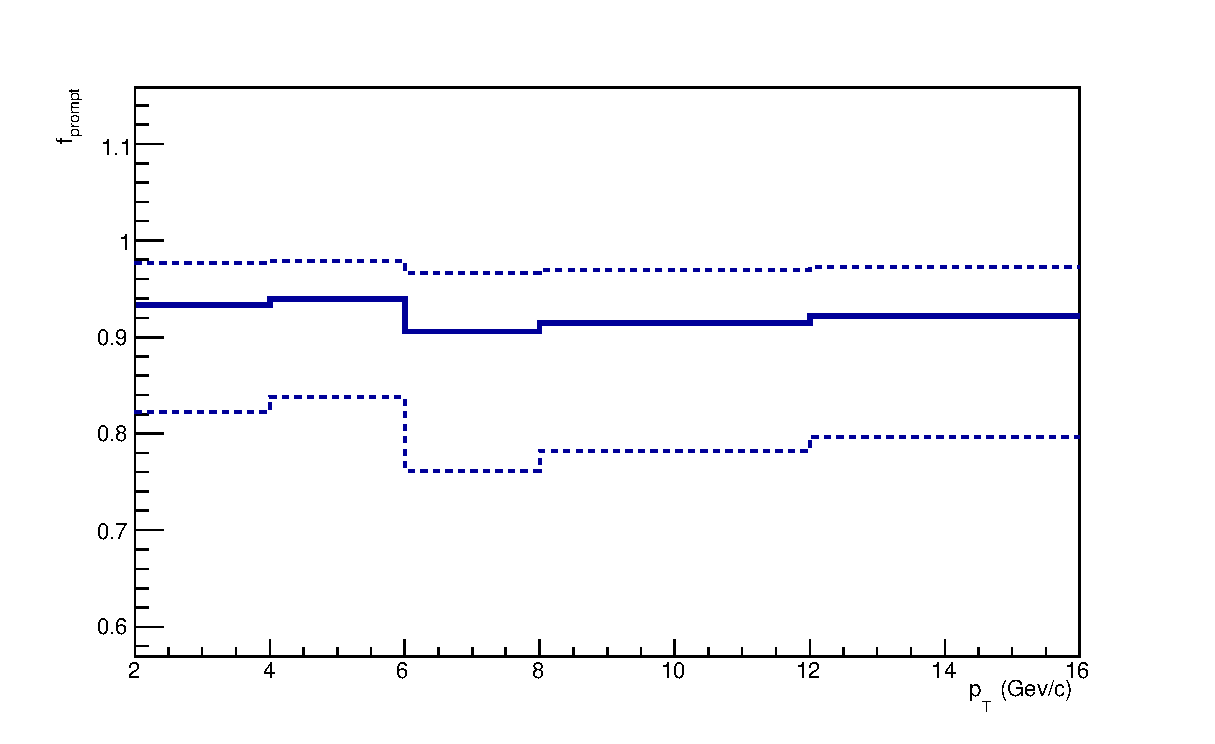
\includegraphics[width=7cm]{FigCap5/fprompt_3050.eps}
\caption{Values of fprompt for the $\Dplus$, $\Dzero$ and $\Ds$ mesons respectively.}
\label{fig:fPrompt}
\end{figure}

\section{Results}

The transverse-momentum distributions d$N$/d$\pt$ of prompt $\Ds$ meson 
is shown in Fig.~\ref{fig:DmesCorrYields010}
for the 0--10\%, 30--50\% and 60--80\% centrality classes. 
The vertical bars represent the statistical uncertainties, the empty boxes
the systematic uncertainties from the data analysis, and the shaded boxes
the systematic uncertainty due to the subtraction of the feed-down from 
B-hadron decays. The uncertainty on the branching ratios is quoted separately.%Uncertainties on the pp cross section
%normalisation and on the branching ratios are quoted separately.

\begin{figure}[!t]
 \begin{center}
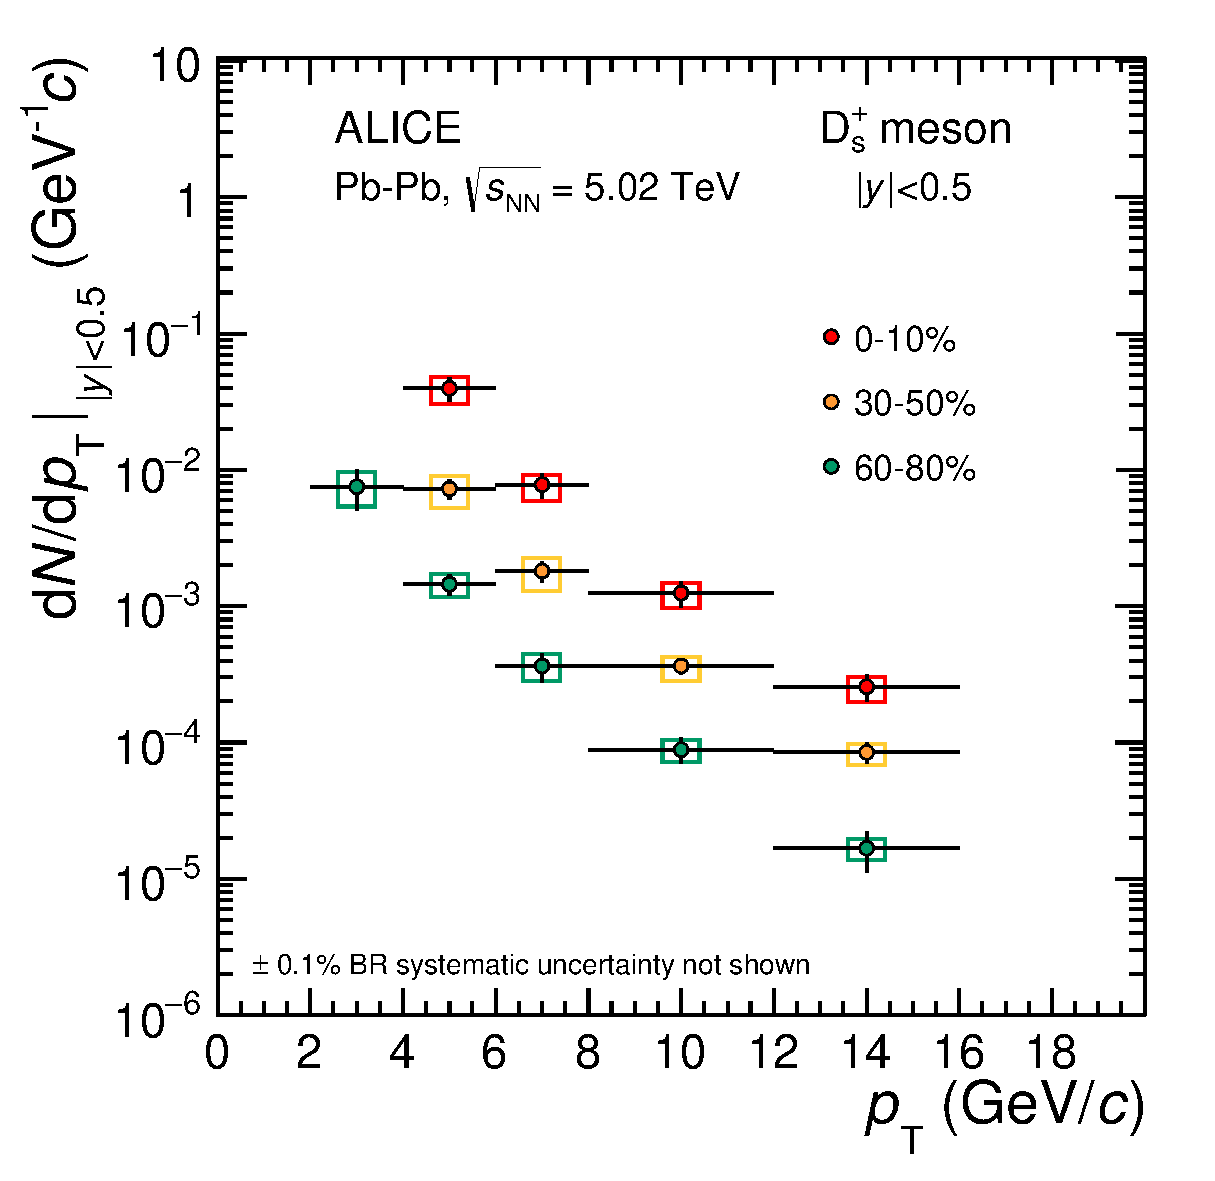
\includegraphics[angle=0, width=7.5cm]{FigCap5/Ds_dNdpt_010_3050_6080.eps}
 \end{center}
 \caption{Transverse momentum distributions d$N$/d$\pt$ of 
prompt $\Dzero$ (a), $\Dplus$ (b), $\Dstar$ (c) and $\Ds$ (d)  mesons in the 0--10\%, 30--50\% and 60--80\% 
centrality classes in $\PbPb$ collisions 
at $\sqrtsNN=5.02~\tev$. 
Statistical uncertainties (bars), systematic uncertainties from data 
analysis (empty boxes) and from feed-down subtraction 
(shaded boxes) are shown. 
Horizontal bars represent bin widths, symbols are placed at the centre of 
the bin. }
 \label{fig:DmesCorrYields010} 
\end{figure} 



Figure~\ref{fig:DmesRatio} shows the $\pt$-dependent ratios of
$\Dplus$/$\Dzero$, $\Dstar$/$\Dzero$, $\Ds/\Dzero$ and $\Ds/\Dplus$ meson yields, 
compared to the values measured in pp collisions at $\sqrt s=7~\tev$~\cite{Acharya:2017jgo}. 
%and central Pb--Pb collisions at $\sqrtsNN=2.76~\tev$~\cite{Adam:2015sza}. 
The $\Dplus$/$\Dzero$ and $\Dstar$/$\Dzero$ ratios are compatible in Pb--Pb and pp collisions, 
indicating no significant modification of their relative abundances. 
The $\Ds/\Dzero$ and $\Ds/\Dplus$ ratios are measured with better precision at 5.02~TeV with respect to 2.76~TeV.
The central values of these ratios are larger in Pb--Pb than in pp collisions, in all three centrality classes, however
the measurements in the two systems are compatible within about one standard deviation of the combined uncertainties.
\iffalse

\begin{figure}[!t]
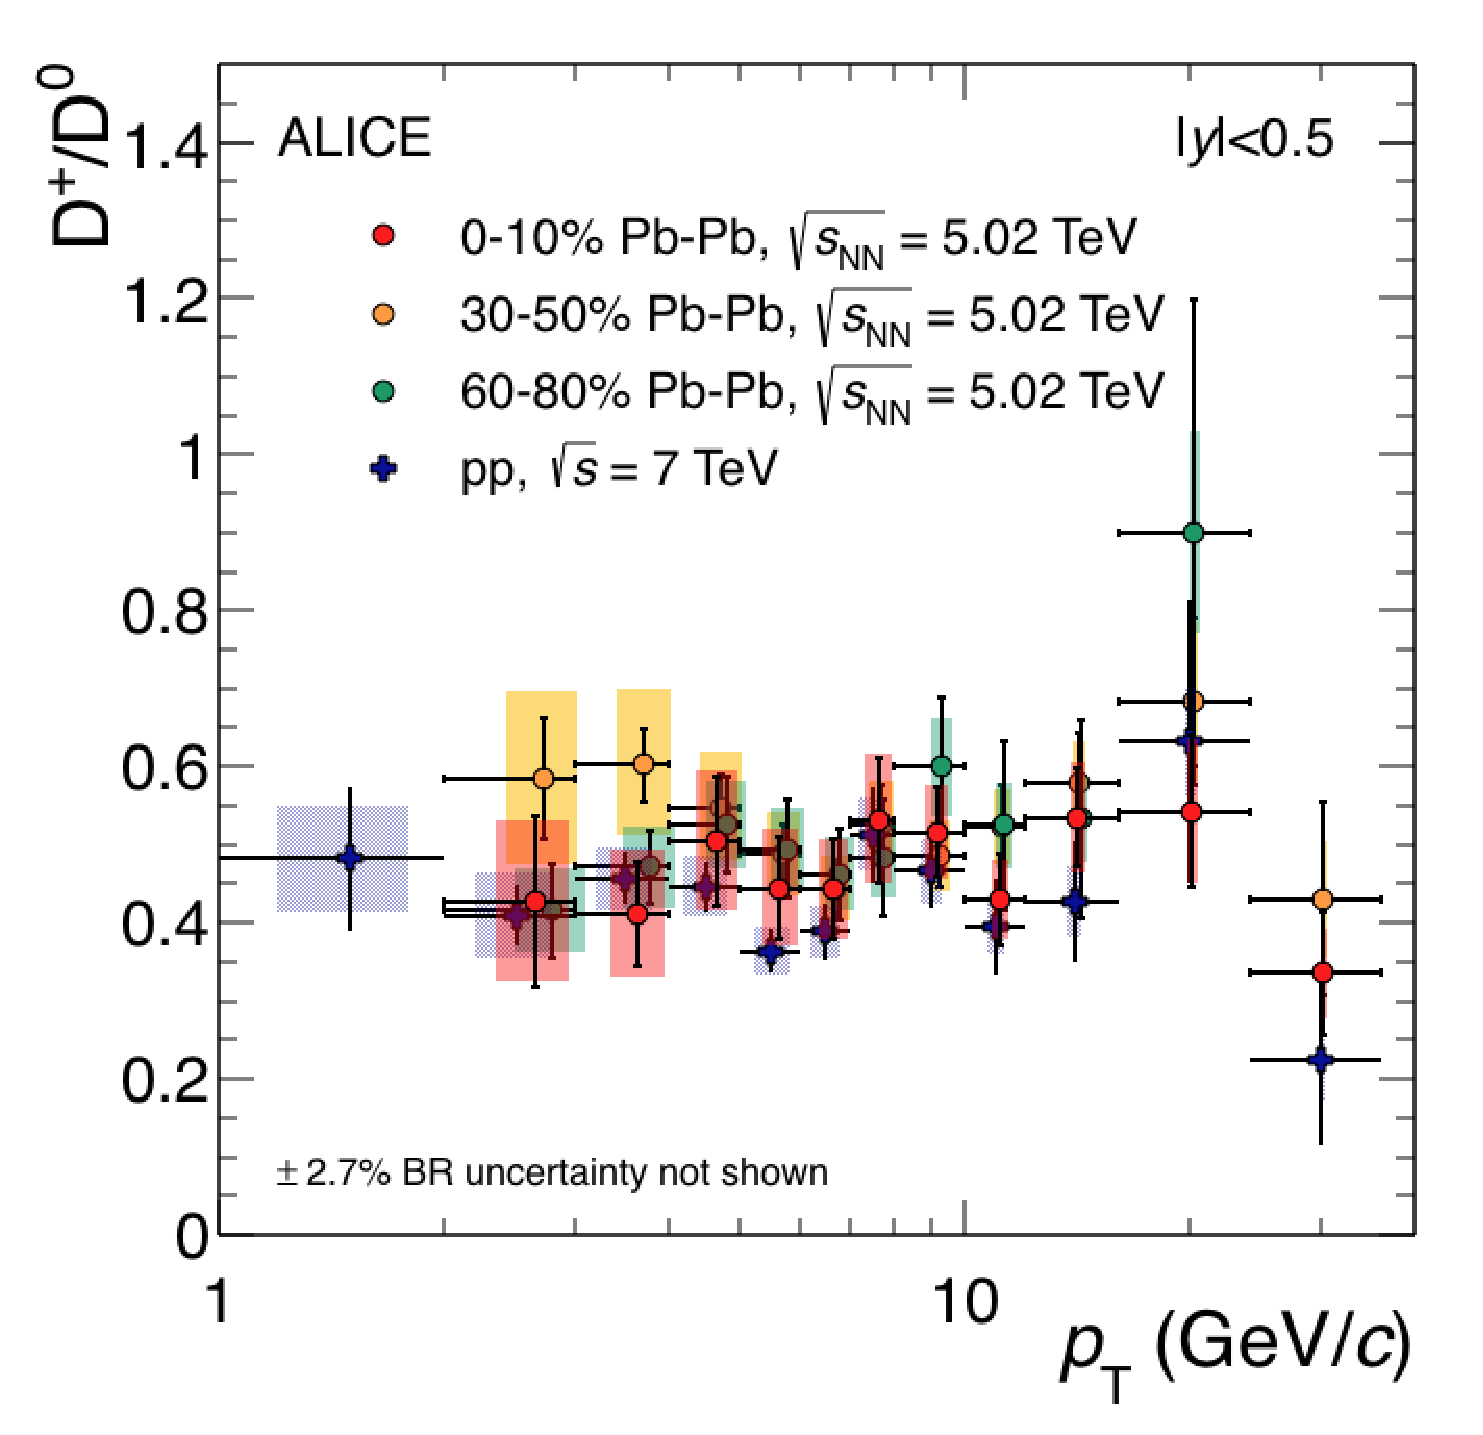
\includegraphics[width=0.49\textwidth]{FigCap5/RatioDplusDzero-PbPb-010-3050-6080-502-pp-7.eps}
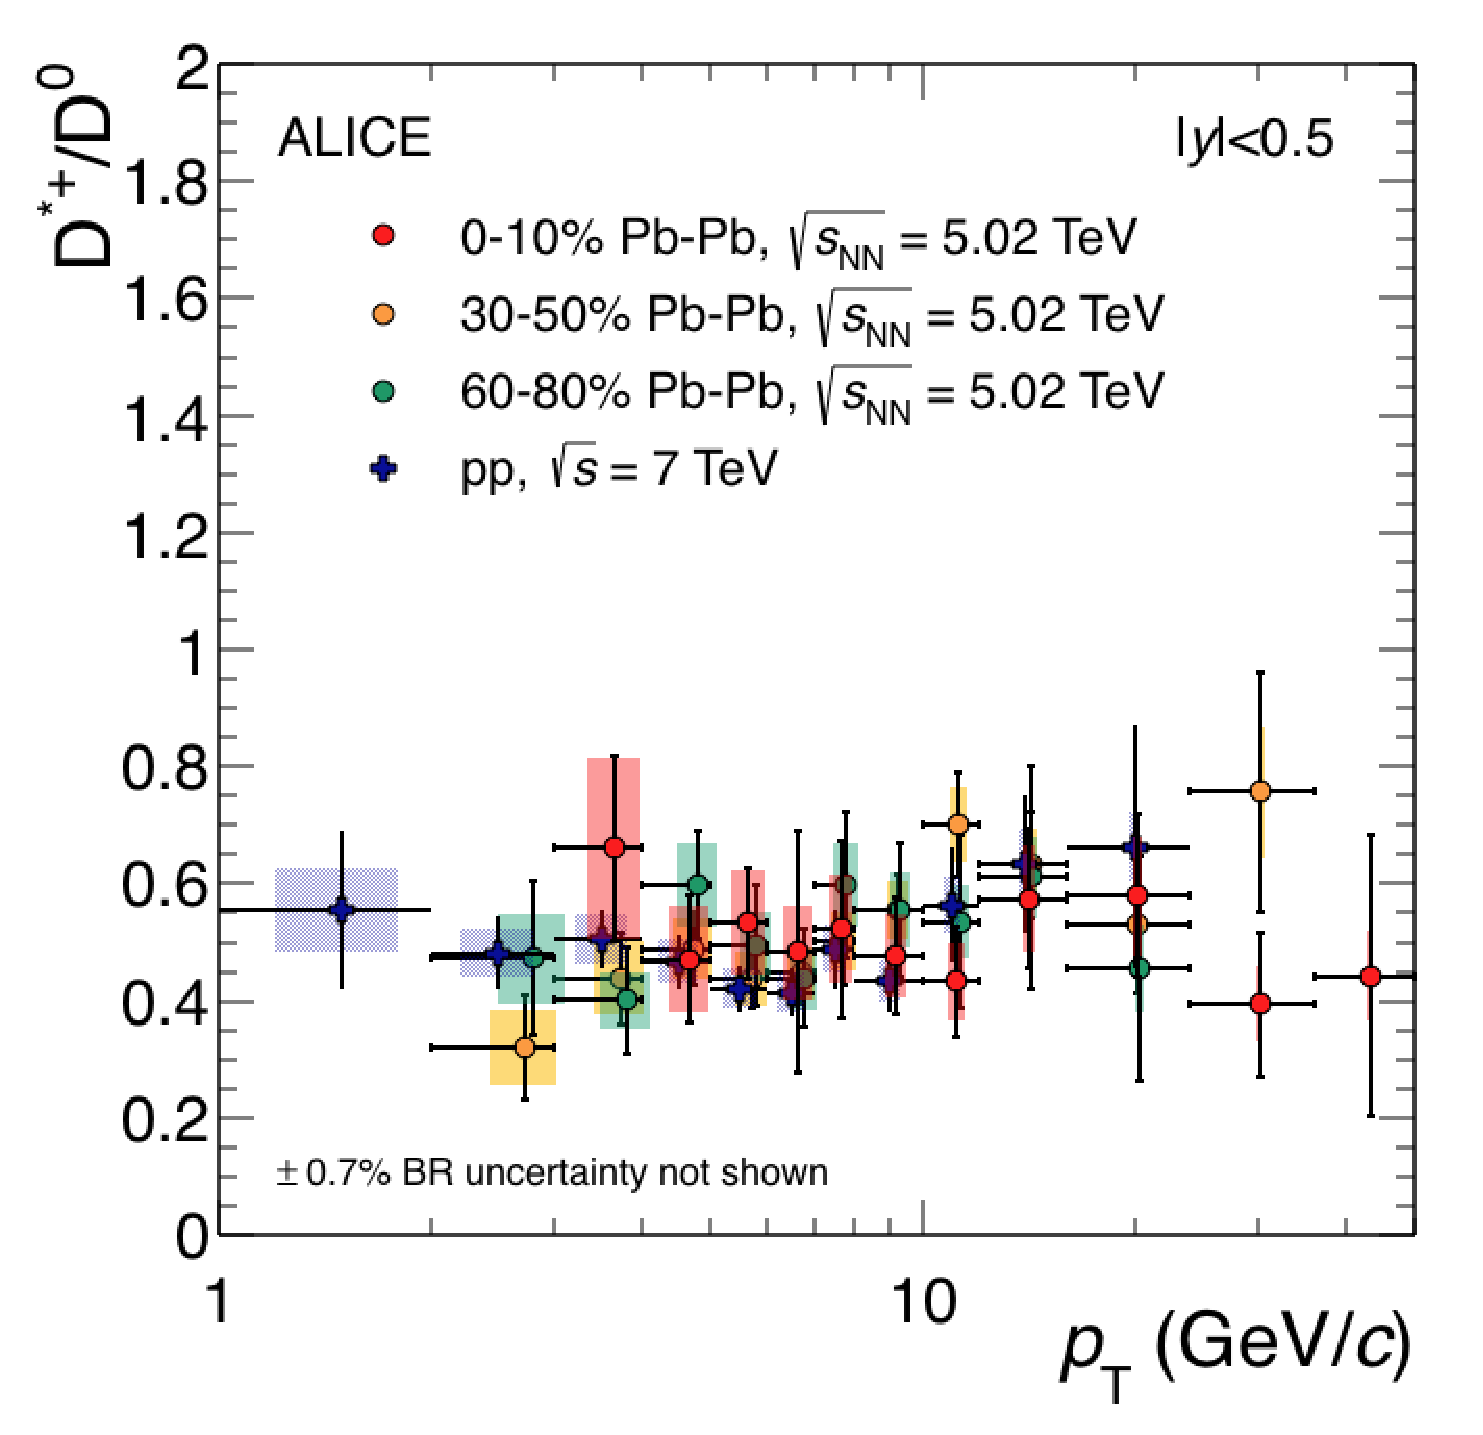
\includegraphics[width=0.49\textwidth]{FigCap5/RatioDstarDzero-PbPb-010-3050-6080-502-pp-7.eps}
 \label{fig:DmesRatio} 
\end{figure} 


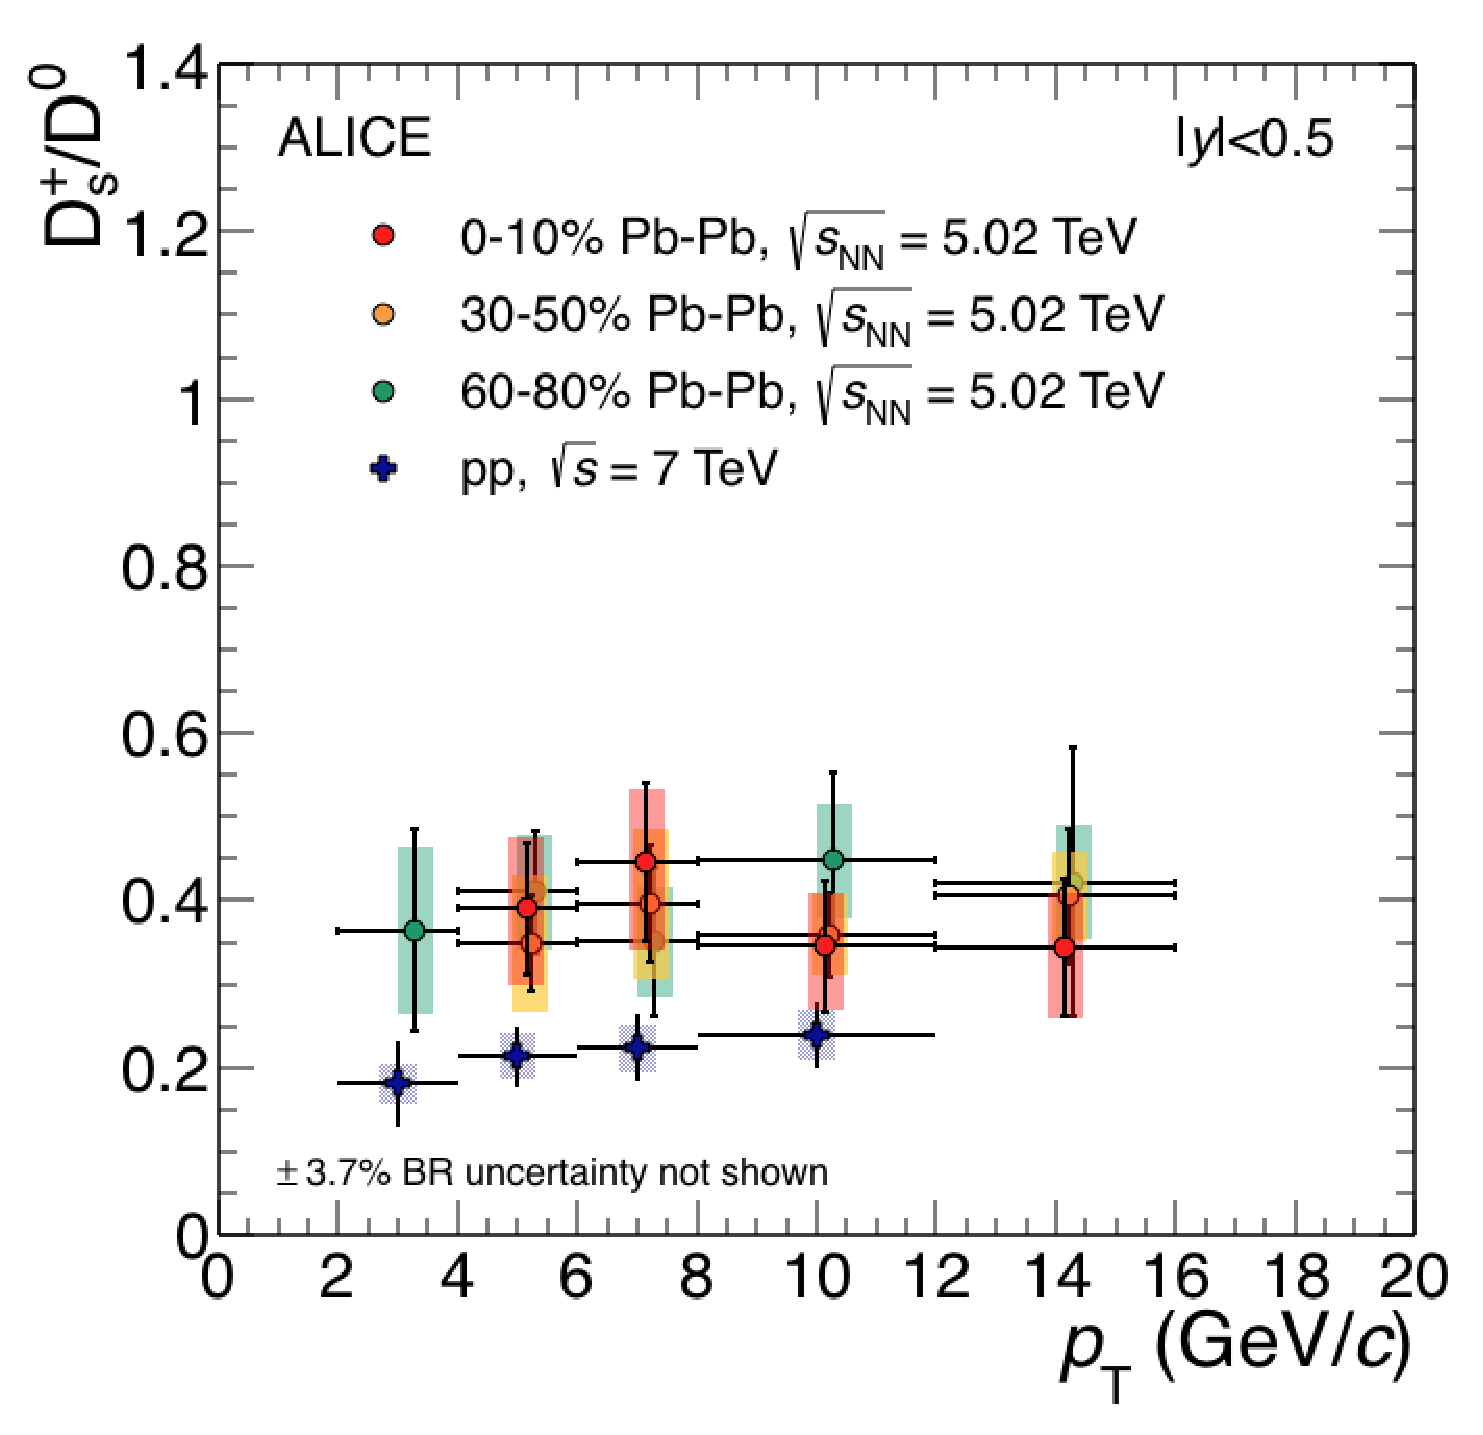
\includegraphics[width=0.49\textwidth]{FigCap5/RatioDsD0-PbPb-010-3050-6080-502-pp-7.eps}
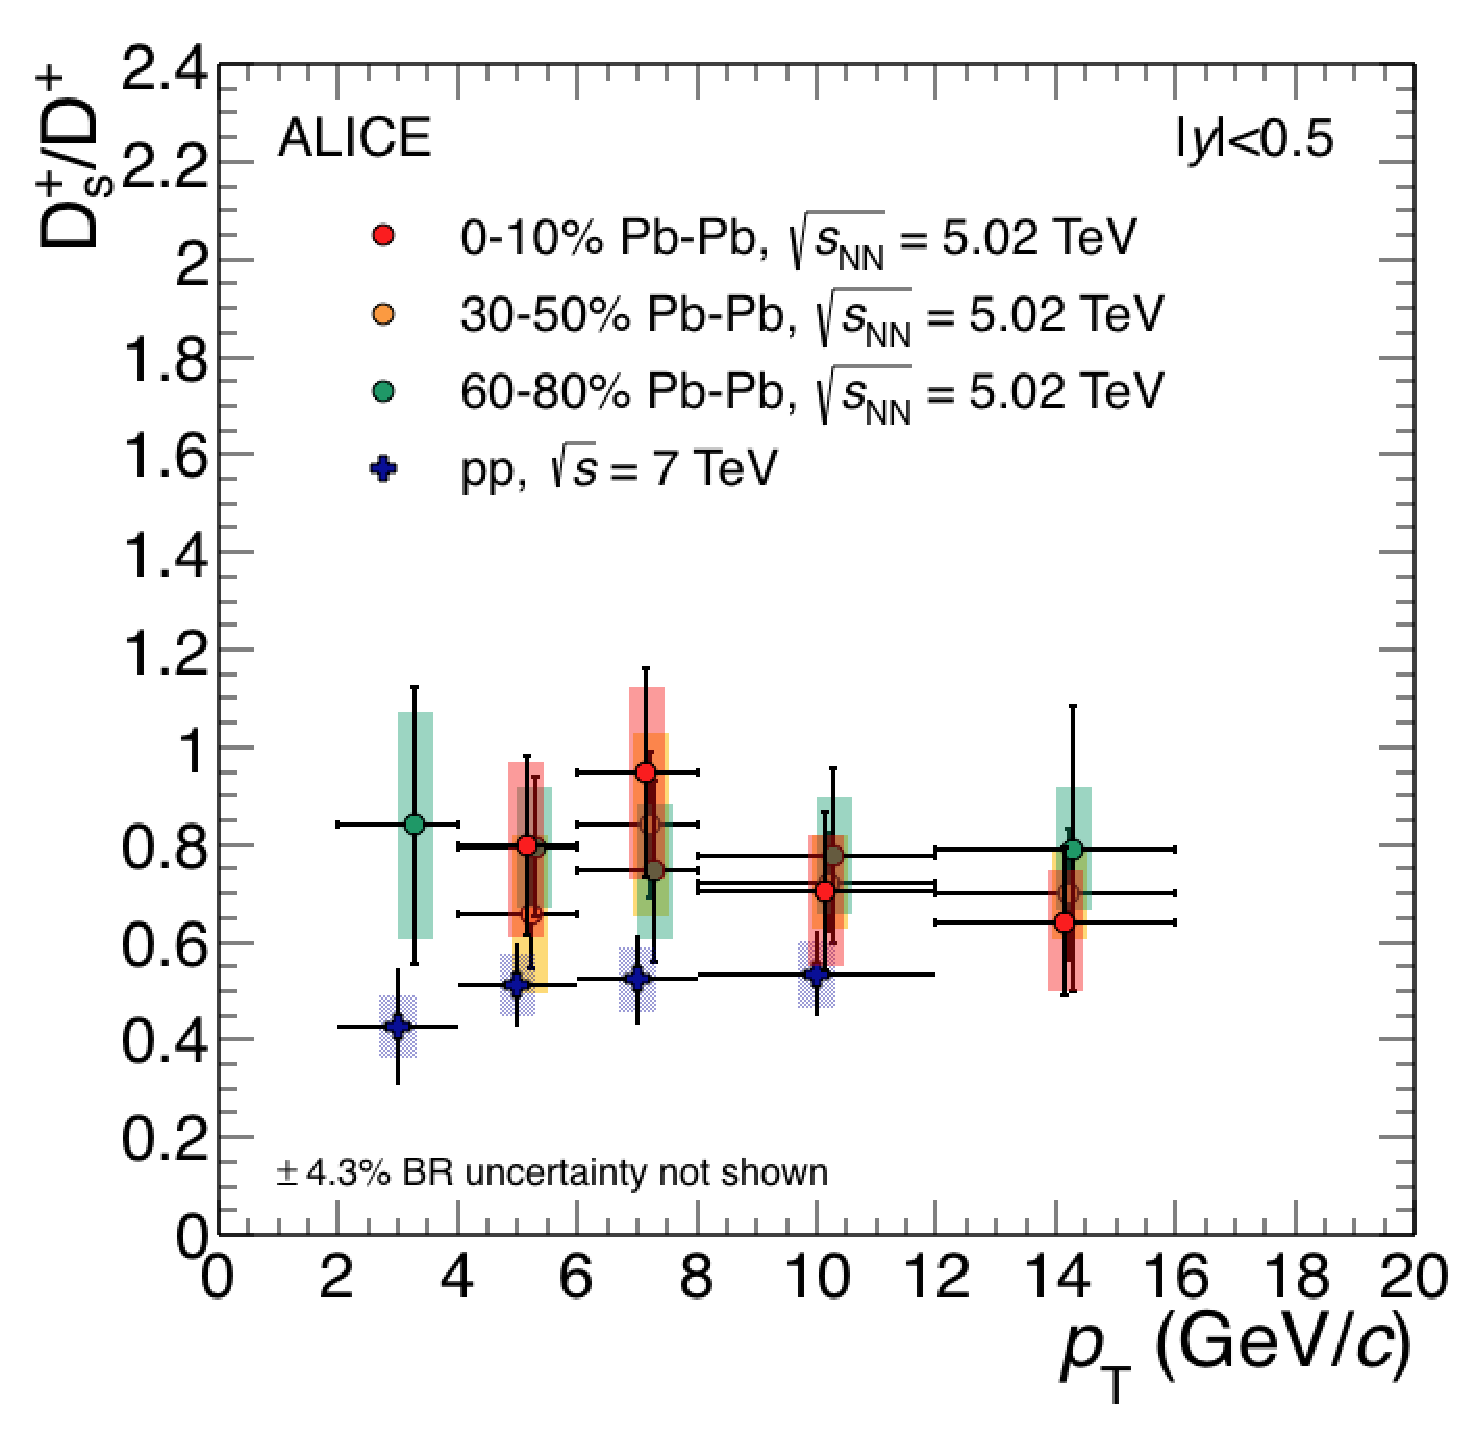
\includegraphics[width=0.49\textwidth]{FigCap5/RatioDsDplus-PbPb-010-3050-6080-502-pp-7.eps}

\begin{figure}[!h]
\centering
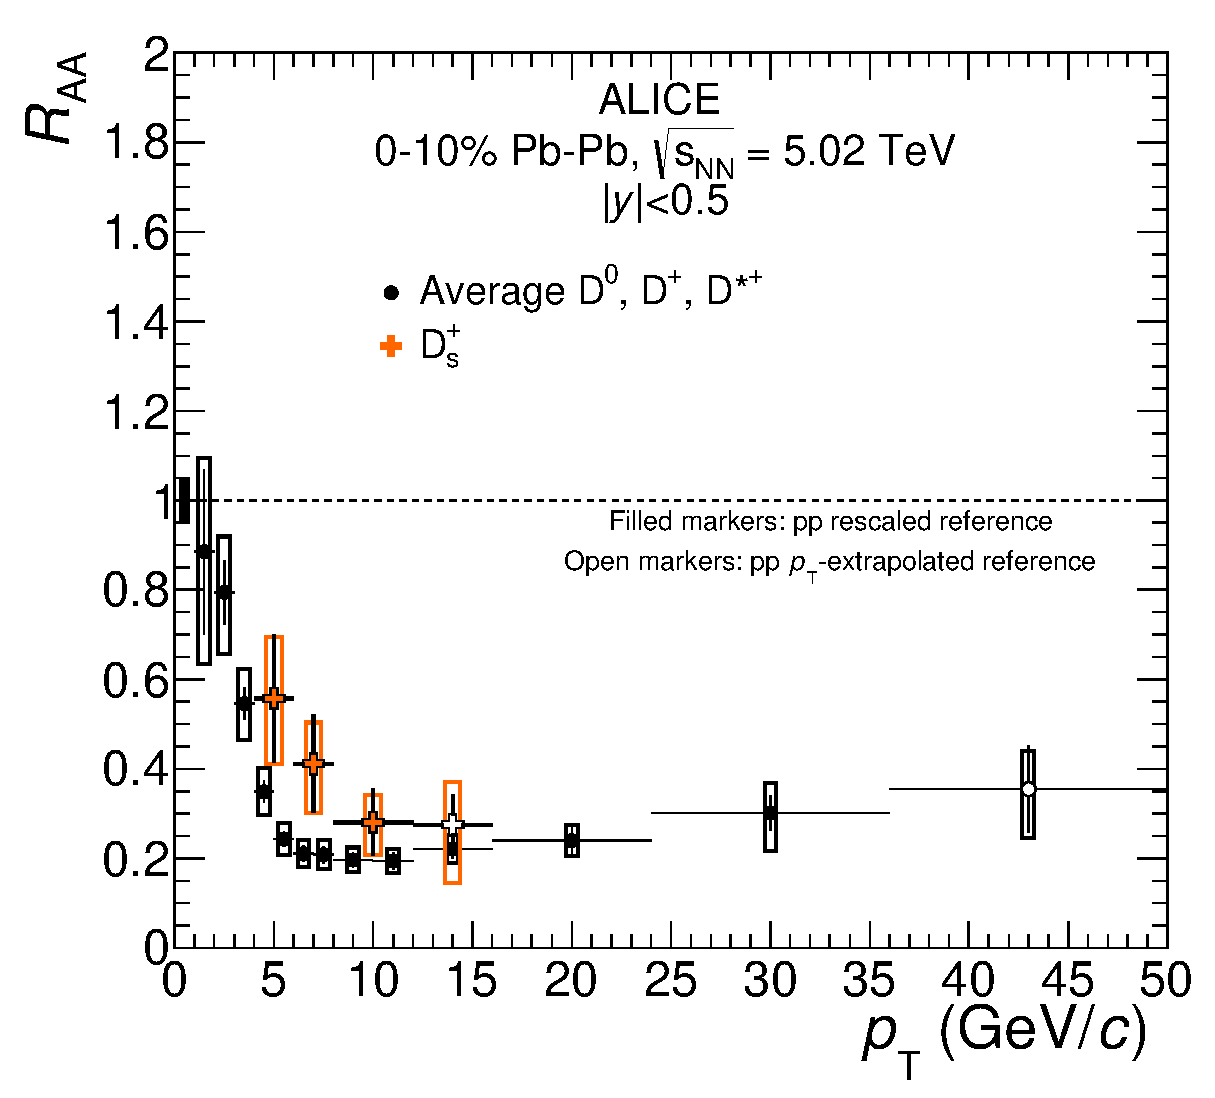
\includegraphics[angle=0, width=0.45\textwidth]{FigCap5/DmesonAverageDs_010_.eps}
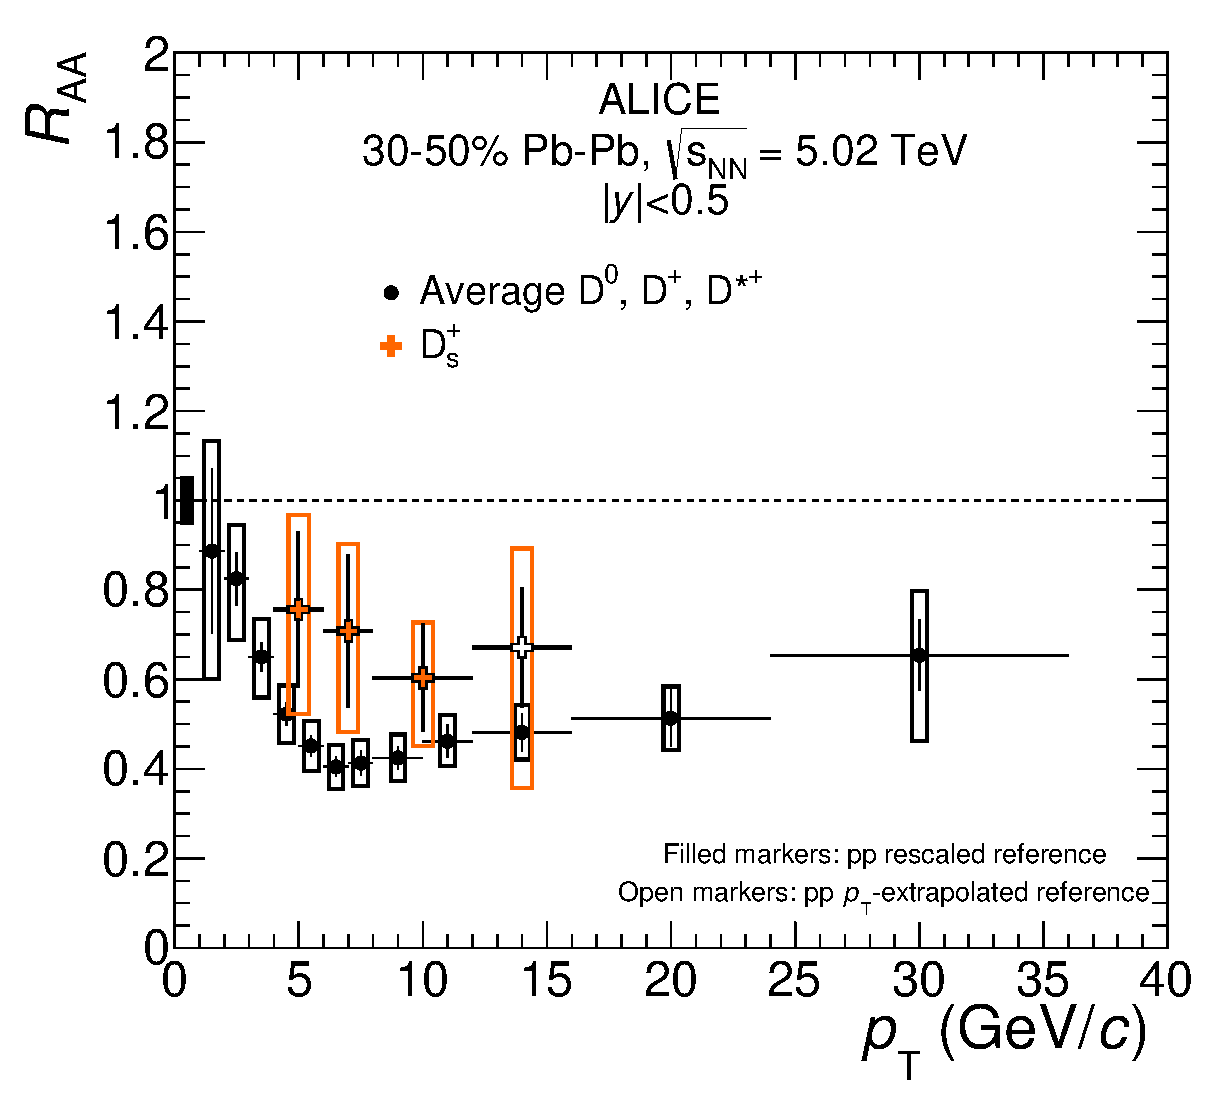
\includegraphics[angle=0, width=0.45\textwidth]{FigCap5/DmesonAverageDs_3050_.eps}
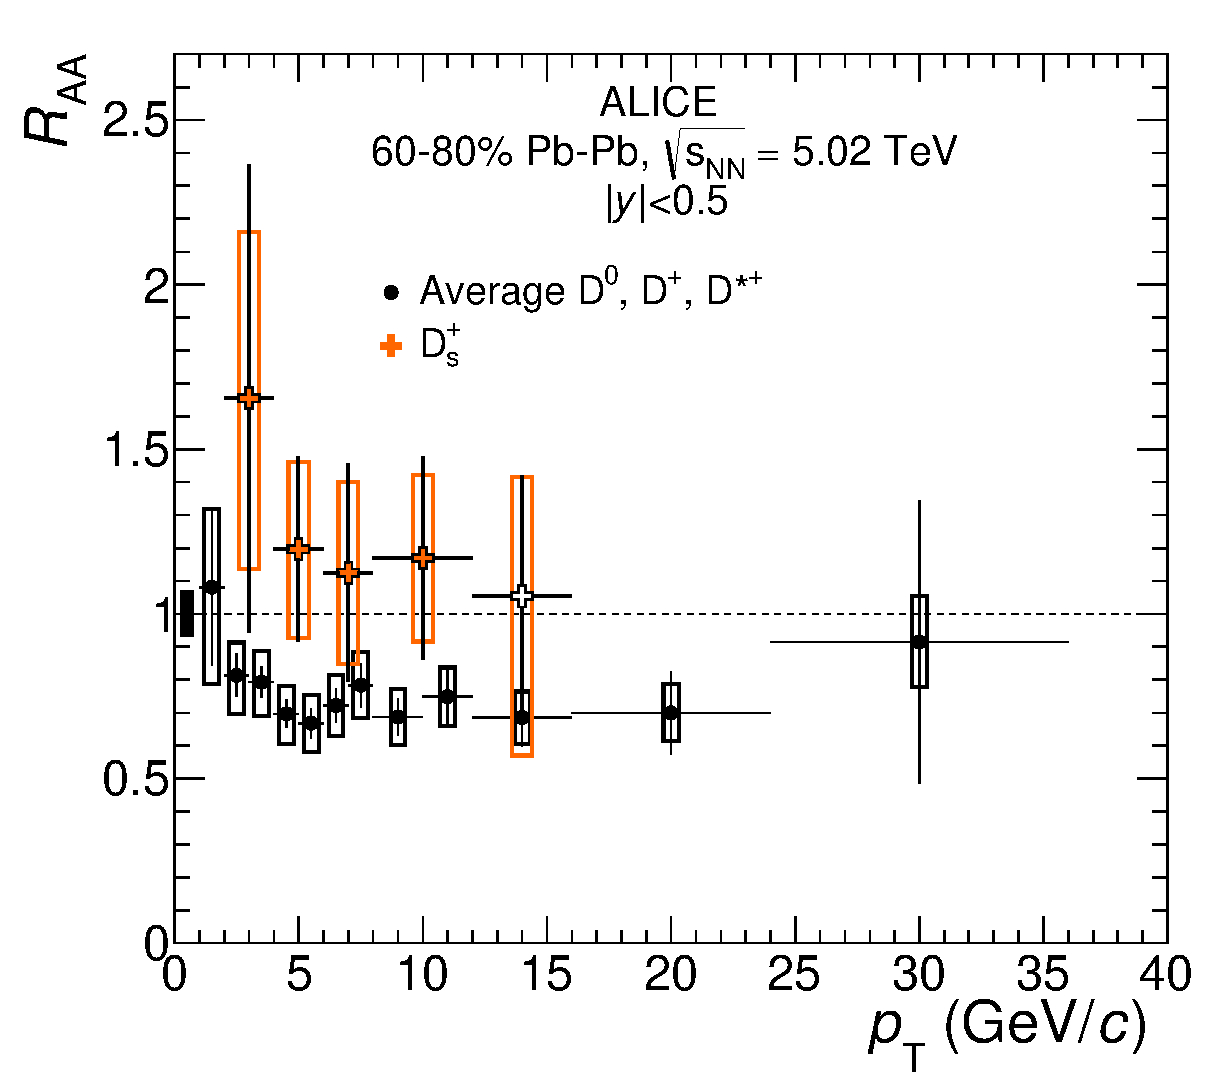
\includegraphics[angle=0, width=0.45\textwidth]{FigCap5/DmesonAverageDs_6080_.eps}
 \caption{$\RAA$ 
  of prompt $\Ds$ mesons 
  compared with the average $\RAA$ of$\Dzero$, $\Dplus$ and $\Dstar$ mesons for the 
0--10\%, 30--50\% and 60--80\%. 
Statistical (bars),  systematic (empty boxes), and normalisation (shaded box) 
uncertainties are shown.}
 \label{fig:DmesRaa} 
\end{figure} 

\fi

The average nuclear modification factors in the 0--10\% and 30--50\% centrality classes (right-hand panels of Fig.~\ref{DmesRaa}) show a suppression that is
maximal at $\pt=6$--$10~\gev/c$, where a reduction of the yields by
a factor of about 5 and 2.5 with respect to the binary-scaled pp reference is observed in the two centrality classes, respectively.
The suppression decreases with decreasing $\pt$ for $\pt<6~\GeV/c$, and 
$\RAA$ is compatible with unity  in the interval $1<\pt<3~\gev/c$.
The average $\RAA$ in the 60--80\% centrality class shows a suppression by about 20--30\%, without a pronounced dependence on $\pt$.

The $\Raa$ of prompt $\Ds$ mesons is shown in the right-hand panels of Fig.~\ref{DmesRaa},
where it is compared with the average $\Raa$ of non-strange D mesons: the central values are
larger for $\Ds$ mesons, but the two measurements are 
compatible within one standard deviation of the combined uncertainties, as in the case of the ratios shown in Fig.~\ref{DmesRatio}.



Models based on heavy-quark transport and models based on perturbative QCD calculations of parton energy loss are shown on the left and on the right, respectively.
Transport models in the left panels include: POWLANG~\cite{Beraudo:2014boa} and TAMU~\cite{He:2014cla}, in which the interactions are only described by collisional (i.e.\,elastic) processes; 
BAMPS-el+rad~\cite{Uphoff:2014hza}, LBT~\cite{Cao:2017hhk} and PHSD~\cite{Song:2015ykw}, in which also energy loss from medium-induced gluon radiation
is considered, in addition to collisional process.
In the right panels, the CUJET3.0~\cite{Xu:2015bbz}, Djordjevic~\cite{Djordjevic:2015hra} and MC@sHQ+EPOS2~\cite{Nahrgang:2013xaa} models include both radiative and collisional energy loss processes, and
the SCET~\cite{Kang:2016ofv} model includes medium-induced gluon radiation and a mechanism of formation and dissociation of heavy-flavour hadrons in the QGP.
All models, with the exception of BAMPS and CUJET3.0, include a nuclear modification of the parton distribution functions.
The LBT, MC@sHQ, PHSD, POWLANG and TAMU
models include a contribution of hadronisation via quark recombination, in addition to independent fragmentation. 
Most of the models provide a fair description of the data in the region $\pt<10~\gev/c$ in central collisions, 
but many of them (LBT, PHSD, POWLANG and SCET) provide a worse description of non-central collisions.
In the high-$\pt$ region above $10~\gev/c$ only the BAMPS, CUJET3.0, Djordjevic and SCET models can describe the data. The CUJET3.0 and Djordjevic models provide a 
fair description of the $\RAA$ in all three centrality classes for $\pt > 5-10~\gev/c$, where radiative energy loss is expected to be the dominant interaction mechanism, suggesting that the dependence of radiative energy loss on the path length of charm quarks in the hot and dense medium is well understood. 

In Fig.~\ref{DandDsRaaWithModels},  the non-strange and strange D-meson $\RAA$ are compared with  
the models that provide both observables. A large increase of the $\Ds$ $\RAA$ is expected in the two models, PHSD and TAMU, in particular for $\pt<5~\gev/c$, with respect to non-strange D mesons. This increase is induced by hadronisation via quark recombination in a strangeness-rich QGP, as well as by different 
interaction cross sections for non-strange D and for $\Ds$ in the hadronic phase of the system evolution. It is interesting  to note that the TAMU model gives a larger effect than the PHSD model and that the central values of the two measured $\RAA$ differ also 
in the region around $\pt=10~\gev/c$, where the effect in the models becomes small, although the present experimental uncertainties prevent us from drawing a firm conclusion. 

The simultaneous comparison of $\RAA$ and elliptic flow $v_2$ measurements at $\sqrtsNN=5.02~\tev$~\cite{Acharya:2017qps} with models can provide more stringent constraints to the implementation of the interaction and hadronisation processes for heavy quarks. 
This comparison is shown in Fig.~\ref{RAAandv2} for the $\RAA$  
and $v_2$, in the 0--10\% and 30--50\% centrality classes respectively, together with models that provide simultaneous description of the observables.
The level of model-to-data consistency was quantified in terms of the reduced $\chi^2$ in the respective $\pt$ interval where the calculations are available.
Values of reduced $\chi^2$ for $\RAA$ measurements in 0--10\% and 30--50\% centrality classes and $v_2$ in 30--50\% centrality class are reported in Table~\ref{tab:RedChi2}.
TAMU model overestimates $\RAA$ at high $\pt$ in central events and describes the magnitude of the elliptic flow, but fails in reproducing the shape.
BAMPS-el overestimates the maximum flow while underestimating the suppression at high $\pt$. The radiative term in BAMPS-el+rad improves the description of the $\RAA$ but gives a smaller than observed maximum $v_2$.~PHSD, POWLANG, LBT and MC@sHQ provide instead a fair description of both $v_2$ magnitude and shape
as well as of energy loss, as their values of $\chi^2/$ndf indeed show. 
	\iffalse

\begin{figure}[!t]
 \begin{center}
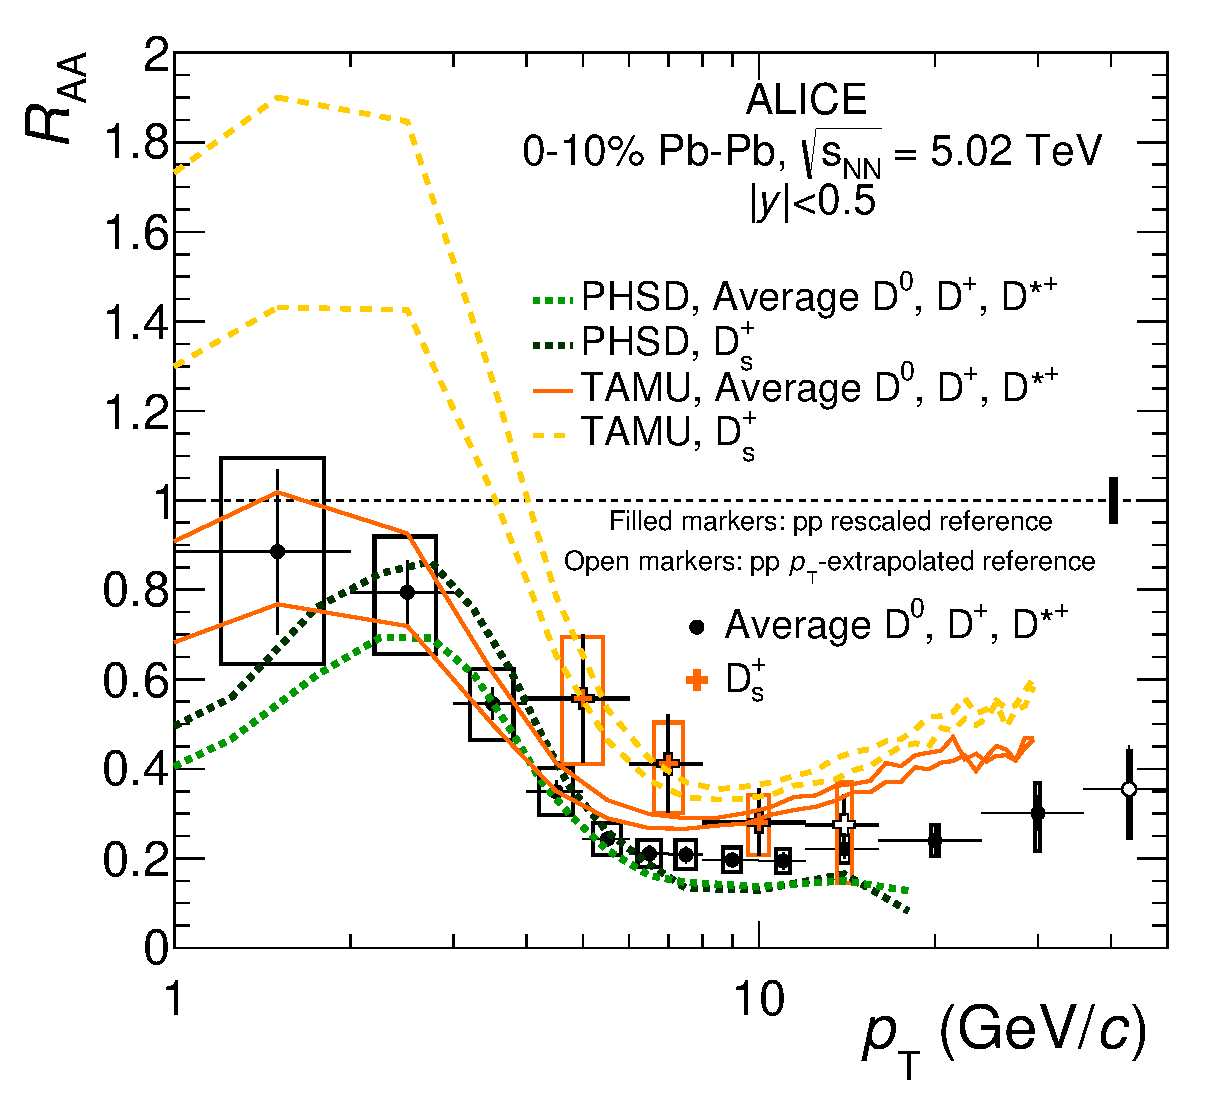
\includegraphics[angle=0, width=0.49\textwidth]{FigCap5/DmesonAverageDs_010_Models_logx_.eps}
 \end{center}
 \caption{Average $\RAA$ of $\Dzero$, $\Dplus$ and $\Dstar$ mesons and $\RAA$ of $\Ds$ mesons in the 0--10\% centrality class compared with the PHSD~\cite{Song:2015ykw}  and TAMU~\cite{He:2014cla} model calculations.}
 \label{DandDsRaaWithModels} 
\end{figure} 

\begin{figure*}[!t]
\begin{center}
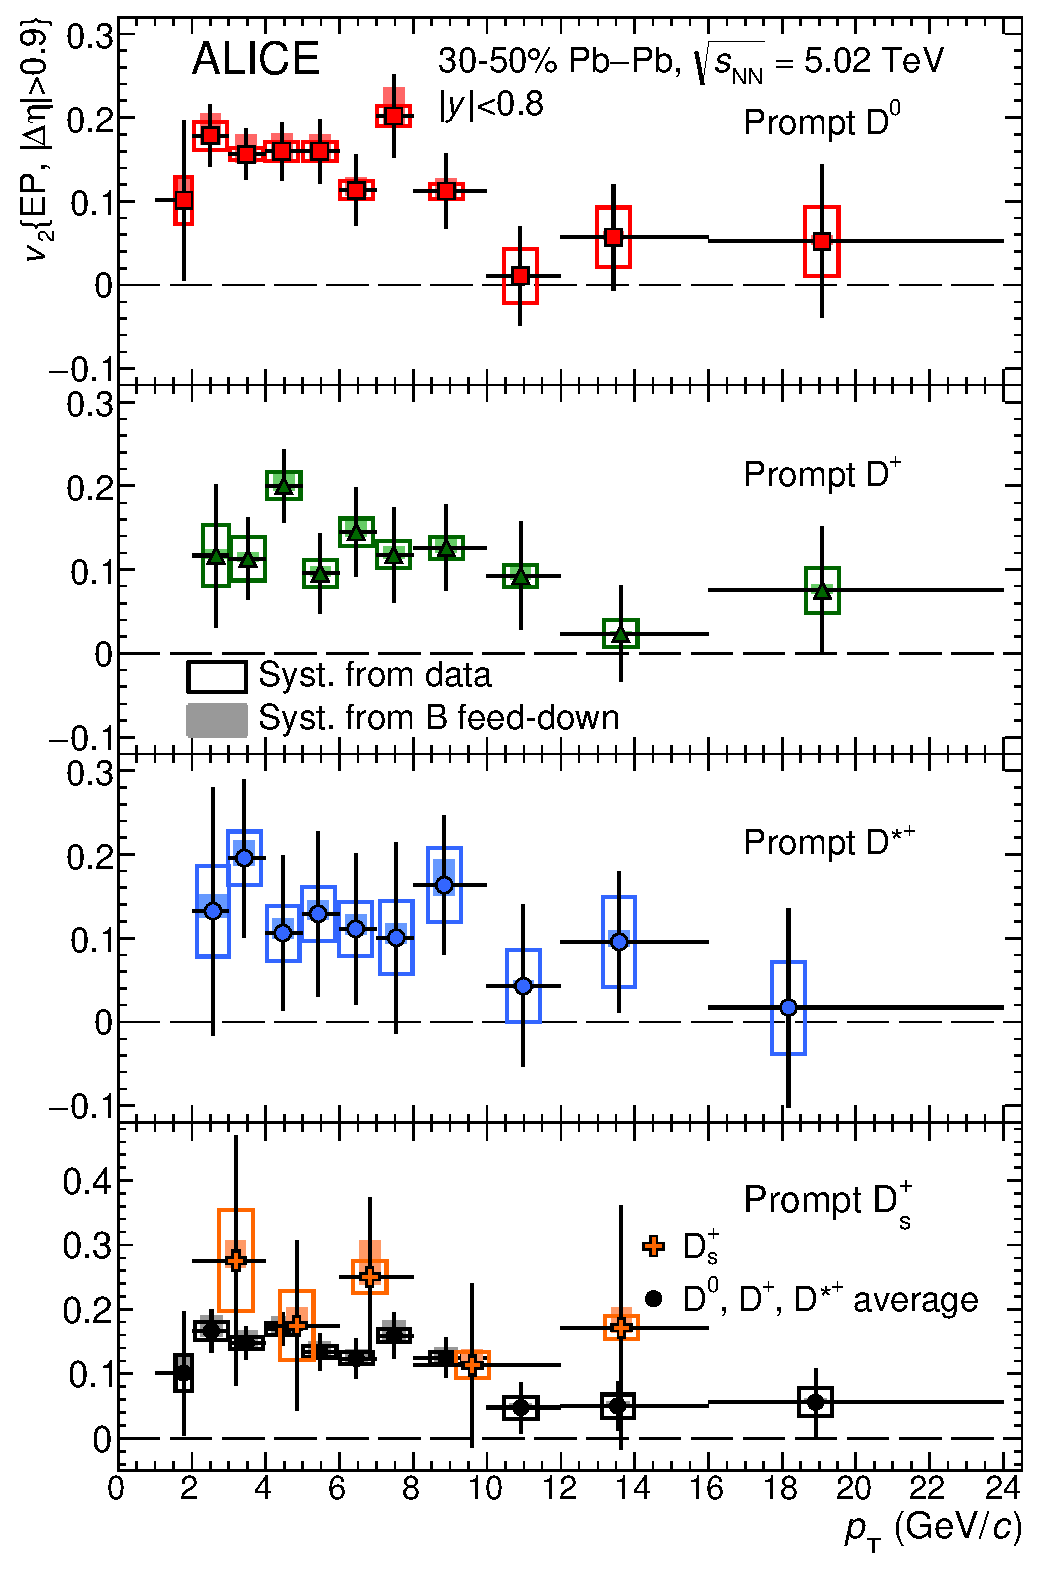
\includegraphics[width=.65\textwidth]{FigCap5/4mesons4pads.eps}
\caption{Elliptic flow $v_2$ as a function of $\pt$ for prompt $\Dzero$, $\Dplus$, 
$\Dstar$ and $\Ds$ mesons and their charge conjugates for $\PbPb$ collisions in the centrality class 30--50\%.
The bottom panel also shows the average
$v_2$ of $\Dzero$, $\Dplus$ and $\Dstar$. The symbols are positioned
horizontally at the average $\pt$ of the reconstructed D mesons. %four D-meson species.
%The central value was obtained with the assumption 
%$v_2^{\rm feed\mbox{-}down}=v_2^{\rm prompt}$.
%The minimum separation in pseudorapidity between D mesons and the particles used to determine $\psi_2$ is indicated ($|\Delta\eta|>0.9$).
Vertical error bars represent the statistical uncertainty, empty boxes the systematic 
uncertainty associated with the D-meson anisotropy measurement and the event-plane 
resolution. Shaded boxes show the feed-down uncertainty.}
\label{fig:v2_4mesons} 
\end{center}
\end{figure*}

\fi
The $v_2$ of prompt $\Dzero$, $\Dplus$, $\Dstar$ and $\Ds$ mesons in
the 30--50\% centrality class is shown as a function of $\pt$ in Fig.~\ref{fig:v2_4mesons}.
%{\bf The meaning of the error bars is described in the figure caption, I would not repeat here.}
The symbols are positioned at the average $\pt$ of the 
reconstructed D mesons: this value was determined as the average of the $\pt$ distribution of candidates in the signal invariant-mass region, 
after subtracting the contribution of the background candidates estimated from the side bands.
The $v_2$ of $\Dzero$, $\Dplus$ and $\Dstar$ are consistent with each other and they are larger than zero in $2<\pt<10~\gev/c$.
The average of the $v_2$ measurements for $\Ds$ mesons in the three $\pt$ intervals within $2<\pt<8~\gev/c$ is positive with a significance of 2.6\,$\sigma$,
where $\sigma$ is the uncertainty of the average $v_2$, calculated using quadratic error propagation for the statistical and uncorrelated systematic uncertainties 
(signal extraction) and linear propagation for the correlated systematic uncertainties ($R_2$ and feed-down correction).
The average $v_2$ and $\pt$ of $\Dzero$, $\Dplus$ and $\Dstar$, shown in the bottom panel of Fig.~\ref{fig:v2_4mesons}, was 
computed using the inverse of the squared statistical uncertainties as weights. 
The systematic uncertainties were propagated by
treating the contributions from $R_2$
and the feed-down correction as correlated among D-meson species. 
